\documentclass[11pt, a4paper]{article}
\usepackage[left= 2.5cm, right = 3cm, bottom = 4 cm]{geometry}
\usepackage[english]{babel}

\usepackage{fancyhdr}
\pagestyle{fancy}
\fancyhead[R]{\thepage}
\fancyhead[L]{\nouppercase{\leftmark}}
\fancyfoot{}

\usepackage{amsthm}
\newtheorem{theorem}{Theorem}[section]
\newtheorem{lemma}[theorem]{Lemma}
\newtheorem{corollary}[theorem]{Corollary}
\newtheorem{definition}[theorem]{Definition}
\newtheorem{algorithm}[theorem]{Algorithm}
\newtheorem*{hypothesis}{Low-Dimensional Trajectory Hypothesis}

\usepackage{amssymb}
\newcommand{\N}{\mathbb{N}}
\newcommand{\R}{\mathbb{R}}	
\newcommand{\A}{\mathcal{A}}
\newcommand{\B}{\mathcal{B}}
\newcommand{\D}{\mathcal{D}}
\newcommand{\F}{\mathcal{F}}
\newcommand{\I}{\mathcal{I}}
\newcommand{\X}{\mathcal{X}}
\newcommand{\Y}{\mathcal{Y}}
\renewcommand{\O}{\mathcal{O}}
\renewcommand{\H}{\mathcal{H}}
\renewcommand{\L}{\mathcal{L}}
\renewcommand{\P}{\mathcal{P}}

\renewcommand{\b}{\mathsf{b}}
\newcommand{\w}{\mathsf{w}}
\newcommand*{\tr}{^{\mkern-1.5mu\mathsf{T}}}

\usepackage{amsmath}
\DeclareMathOperator*{\argmin}{arg\,min}
\DeclareMathOperator*{\argmax}{arg\,max}
\DeclareMathOperator*{\E}{\mathbb{E}}

\usepackage{graphicx, scrextend, algorithmic, xcolor, mathabx, tabu, multirow, colortbl, subfigure}

\usepackage[ruled]{algorithm}

\setlength{\parindent}{0em} 

%%%%%%%%%%

\begin{document}

\tableofcontents
\thispagestyle{empty}

\pagebreak
\section{Introduction}

This thesis is about...

\pagebreak
\section{Neural Networks}

This section introduces the basic concepts of neural networks and provides the necessary notation for further sections. We start with the formal definition of neural networks and explain the process of training afterwards. Finally we will introduce several training methods.

\subsection{Notation} \label{sec:notation}

To start things off, we consider the simple model of a neuron. 

\begin{definition}
Let $n_x \in \N$, $\w \in \R^{n_x}$, $\b \in \R$ and $\sigma: \R \to \R$. A neuron is defined as
\[ \nu : \R^{n_x} \to \R : x \mapsto \sigma \Big ( \w \tr x + \b \Big ).\] % \sigma \Big ( \sum_{i=1}^{n} w_ix_i + b \Big ) =
In this notion $\sigma$ is called the activation function, $\w$ the weights and $\b$ the bias of $\nu$.
\end{definition}

As a generalization of this concept, one can use multiple neurons in parallel to form a layer.

\begin{definition}  \label{def:layer}
Let $n_x, n_y \in \N$, $W = [\w_1, \dots, \w_{n_y}] \in \R^{n_x \times n_y}$, $\b \in \R^{n_y}$ and $\sigma : \R \to \R$. Given neurons $\nu_i$ with weights $\w_i$, bias $\b_i$ and activation function $\sigma$ for $i=1, \dots, n_y$, we define a layer as
\[ f : \R^{n_x} \to \R^{n_y} : x \mapsto \begin{bmatrix} \nu_1(x) \\ \vdots \\ \nu_{n_y}(x) \end{bmatrix} = \sigma \Big ( W\tr x + \b \Big ), \]
where the activation function $\sigma$ is applied element-wise.
\end{definition}

To provide a better understanding, these basic concepts can be visualized as graphs.

\begin{figure}[!h]
\begin{minipage}[c]{0.5\textwidth}
\centering
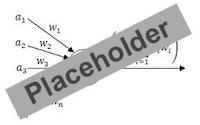
\includegraphics[width=0.9\textwidth]{images/neuron.png}
      	\caption{Illustration of a neuron as graph.}
\end{minipage}
\begin{minipage}[c]{0.5\textwidth}
\centering
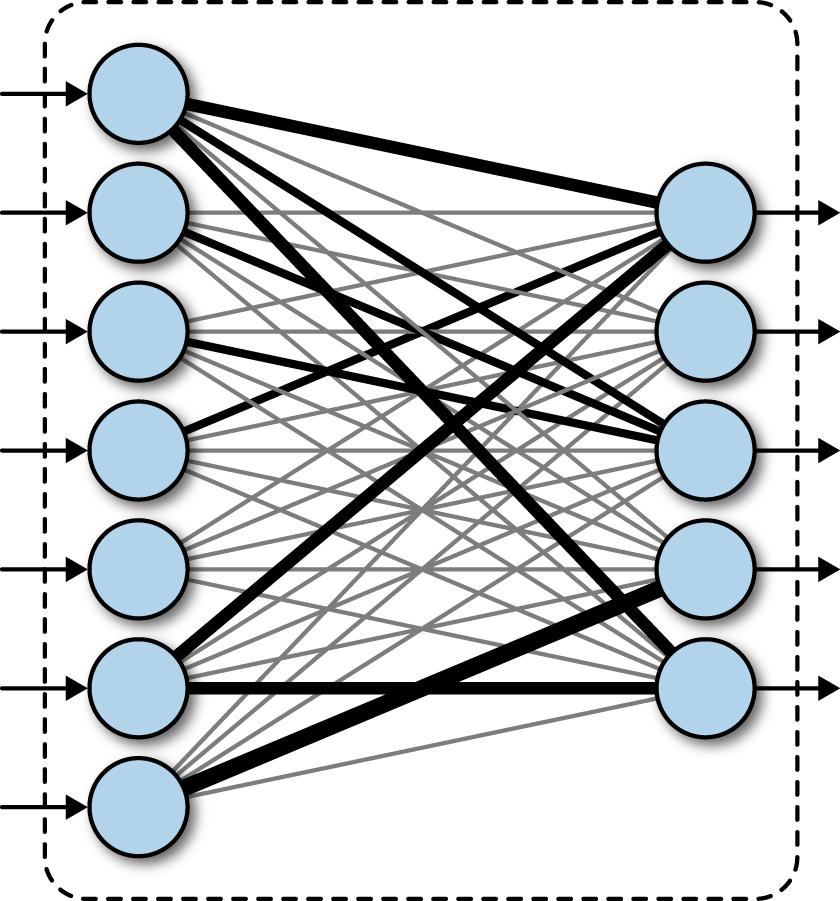
\includegraphics[width=0.9\textwidth]{images/layer.png}
      	\caption{Illustration of a layer as graph.}
\end{minipage}
\end{figure}

In the following we will no longer distinguish between weights and biases and simply refer to them as parameters. Logically one can use the output of a layer as input for another layer. Iteratively doing so will construct specific functions known as neural networks. In order to formalize this idea we denote the following definition. \\ \\

\begin{definition} \label{def:network}
Let $l \in \N$ and $n_0, \dots, n_l \in \N$. A neural network is defined as a function
\[ f : \R^{n_0} \to \R^{n_l} : x \mapsto f^{(l)} \circ f^{(l-1)} \circ \cdots \circ f^{(1)} (x),\]
where $f^{(i)}$ for $i=1, \dots, l$ is a layer with input dimension $n_{i-1}$ and output dimension $n_i$. Networks with a certain level of complexity, say $l>2$, are referred to as deep neural networks.
\end{definition}

Just like neurons and layers, neural networks can also be visualized as graphs.

\begin{figure}[!h]
\centering
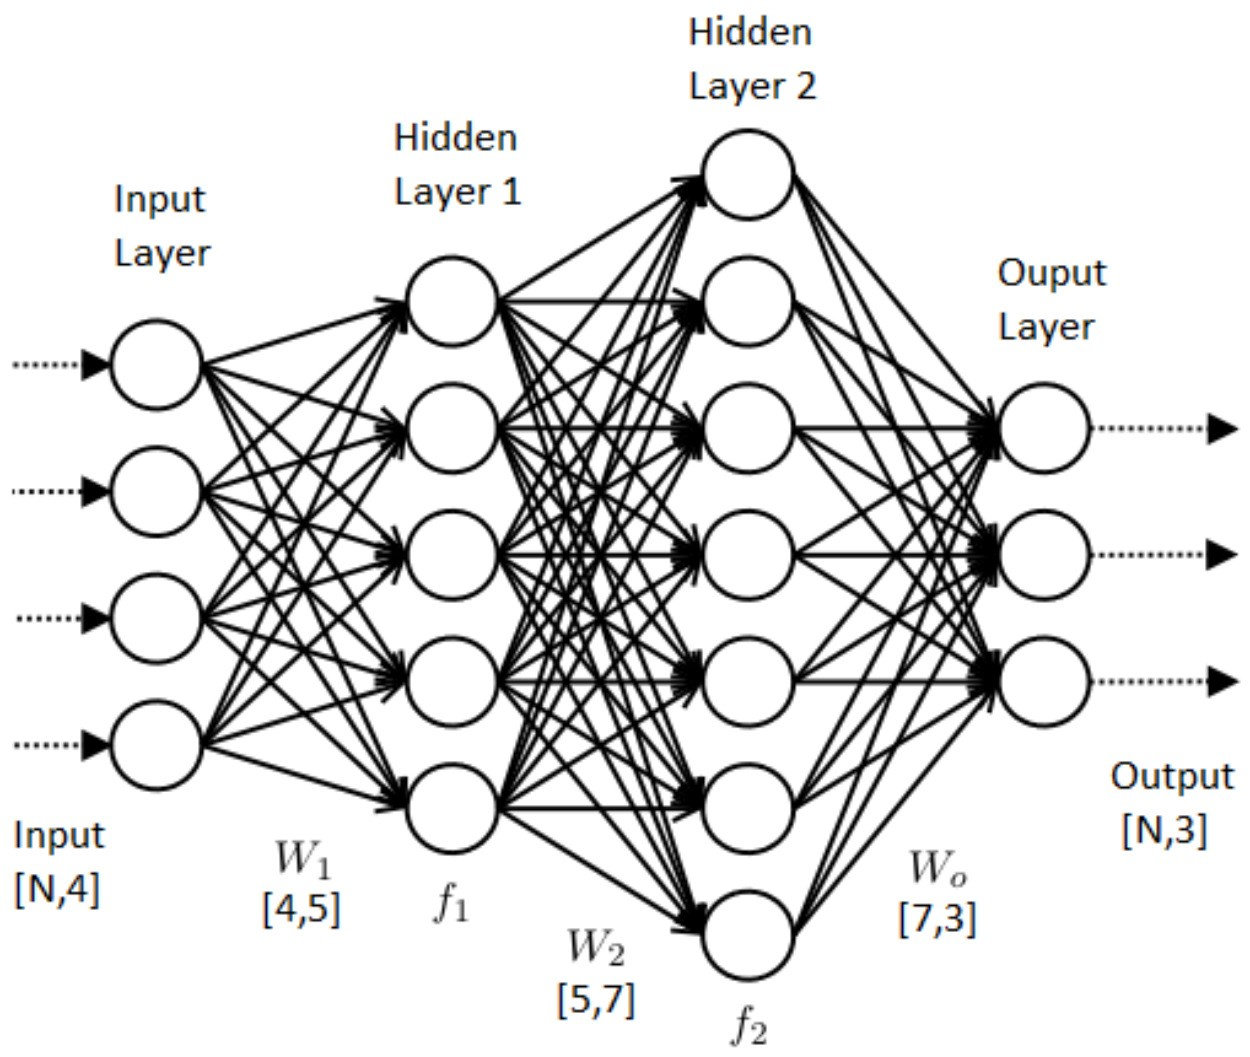
\includegraphics[width=0.6\linewidth]{images/network.png}
\caption{Illustration of a neural network as graph.}
\label{fig:neuron}
\end{figure}  

Neural networks find massive adoption in machine learning as they can model arbitrary complex functions. For example one could envision functions that predict the weather at a specific place and time or functions that determine if an image contains a cat or a dog. Clearly there is no simple mathematical formula to describe such problems. \\

A common practice to learn those functions is, to fix the number of layers, the number of neurons per layer as well as the activation functions, to choose some initial parameters and then iteratively adjust the parameters in order to approximate the unknown target function. In the notion of definition \ref{def:network} one can determine the total number parameters in $f$ as
\[ n = \sum_{i=0}^{l-1} (n_i + 1) \cdot n_{i+1}. \]
Denoting these parameters as a vector $w \in \R^n$ enables us to define a function
\[ \tilde{f} : \R^{n_0} \times \R^n \to \R^{n_l} : (x,w) \mapsto \tilde{f}(x,w), \]
such that for fixed $w_1, w_2 \in \R^n$ the functions $\tilde{f}(x,w_1)$ and $\tilde{f}(x,w_2)$ are neural networks matching in their number of layers, number of neurons as well as activation functions and differing only in their choice of parameters. One calls $\tilde{f}(x,w_1)$ and $\tilde{f}(x,w_2)$ realizations of the neural network architecture $\tilde{f}$. \\

In the following, the terms neural network and neural network architecture will be used synonymously if the meaning is clear by the context. Unless otherwise specified, $n_0 \in \N$ will denote the dimension of the input space, $n_l \in \N$ will denote the dimension of the output space and $n \in \N$ will denote the number of adjustable parameters.

\subsection{Training in the Parameter Space}\label{sec:Training}

Training a neural network refers to finding the optimal parameters, given a fixed neural network architecture $\tilde{f} : \R^{n_0} \times \R^n \to \R^{n_l}$. In other words, finding a function $f \in \F|_{\tilde{f}}$, where
\[ \F|_{\tilde{f}} \coloneq \Big \{ f_w : \R^{n_0} \to \R^{n_l} : x \mapsto \tilde{f}(x,w) \mid w \in \R^n \Big \} \]
denotes the set of all neural networks with given architecture. In order to define a sense of optimality, we need a mechanism measuring the quality of network outputs. This is done by a loss function
\[ \ell: \R^{n_l} \times \R^{n_l} \to \R_+ : \big ( f(x,w),y \big ) \mapsto \ell \big ( f(x,w),y \big ) ,\]
that should be chosen in such a way, that for some input $x \in \R^{n_0}$ with target output $y \in \R^{n_l}$ it associates some cost with the error between the prediction $f(x,w)$ and the true label $y$. \\

Under the assumption, that in reality there exists a probability distribution $\D$ on $\R^{n_0} \times \R^{n_l}$, describing the correlation between inputs $x \in \R^{n_0}$ and target values $y \in \R^{n_l}$, we call a parameter vector $w_* \in \R^n$ to be optimal, if
\[ \forall w \in \R^n : R(w_*) \leq R(w), \]
where $R(w)$ denotes the so called risk or generalization error 
\[ R : \R^n \to \R_+ : w \mapsto \E_{(x,y) \sim \D } \Big [ \ell \big (f(x,w),y \big ) \Big ]. \]

For later use we will denote the marginal distribution of the inputs as $\D_x$. At this point it should be noted, that in general the underlying probability distribution $\D$ is unknown. Hence we can not evaluate the expectation in previous expression. \\

For this reason, the training of neural networks requires a set of $m \in \N$ labeled samples
\[ \Big \{ (x_i,y_i) \in \R^{n_0} \times \R^{n_l} \mid i=1, \dots, m \Big \}, \]
which is called training data. Instead of working with the generalization error, the training data enables us to minimize the empirical error function
 \[ E : \R^n \to \R_+ : w \mapsto \frac{1}{m} \sum_{i=1}^{m} \ell \big ( f(x_i,w),y_i \big) + \lambda \big \| w \big \|_2^2, \]
where $\lambda \geq 0$ is some regularization parameter used to control the complexity of $w$. \\
 
Intuitively, minimization of the empirical error should lead to a minimization of the generalization error as well. Currently, a lot of research is being done on how these measures relate to each other. Nevertheless this thesis will focus on how to minimize the empirical error given labeled training data. \\

The problem of finding some parameter vector $w$ that minimizes the empirical error function is usually hard to solve as the error may have highly nonlinear dependencies on the parameters. This is why in practice one often aims to compare several local minima and to settle for one that is sufficient enough, regardless of whether it is a global minimum or not.

\begin{definition}
Let $f: \R^n \to \R$ be differentiable. The gradient of $f$ is defined as
\[ \nabla f : \R^n \to \R^n : x = (x_1, \dots, x_n) \mapsto \bigg [ \frac{\partial}{\partial x_1} f(x), \cdots, \frac{\partial}{\partial x_n} f(x) \bigg ]\tr . \]
\end{definition}

Due to the complexity of the error function, in general there is no easy way to find an analytical solution to the problem $\nabla E(w) = 0$. Hence most of the techniques for error minimization are based on iterative approximation. One popular method is gradient descent, which was first raised by Cauchy in \cite{GD}.

\begin{algorithm}
\caption{Gradient Descent \textcolor{white}{$\Big |$}} \ \\
\textcolor{white}{$\Big |$}\textbf{Input:} Differentiable $f: \R^n \to \R$, $x_0 \in \R^n$, $\epsilon \geq 0$ \\
\textcolor{white}{$\Big |$}1: Initialize $k \leftarrow 0$; \\
\textcolor{white}{$\Big |$}2: \textbf{while} $ \big \| \nabla f(x_k) \big \|_2 > \epsilon $ \textbf{do}:\\
\textcolor{white}{$\Big |$}3: \quad Choose a step size $\eta_k > 0$; \\
\textcolor{white}{$\Big |$}4: \quad Set $x_{k+1} \leftarrow x_k - \eta_k \cdot \nabla f(x_k)$ and $k \leftarrow k+1$; \\
\textcolor{white}{$\Big |$}5: \textbf{end while}
\end {algorithm}

We will see, that in the case where $f$ is bounded from below and $\nabla f$ is Lipschitz continuous, we can guarantee the  convergence of gradient descent to a stationary point.

\begin{definition}
Let $(\X,d_{\X})$ and $(\Y, d_{\Y})$ be two metric spaces. A function $f: \X \to \Y$ is called Lipschitz continuous, if there exists $L \geq 0$, such that
\[ \forall x,x' \in \X : d_{\Y} \big ( f(x) , f(x') \big ) \leq L \cdot d_{\X}(x,x'). \]
The smallest constant $L$, that suffices the previous condition is called Lipschitz constant of $f$.
\end{definition}

Casually speaking, the Lipschitz continuity of $\nabla f$ ensures that the gradient does not change heavily for two points that are close to each other.

\begin{definition}
Let $f: \R^n \to \R$ be differentiable. A stationary point of $f$ is an element of
\[ \big \{ x \in \R^n \mid \nabla f(x) = 0 \big \}. \]
\end{definition}

There a three kinds of stationary points: saddle points, local extrema and global extrema. We are especially interested in global minima as they provide the lowest possible error.

\begin{definition}
Let $\X$ be a subset of some real vector space and $f: \X \to \R$ be bounded from below. We call $x_* \in \X$ a global minimizer of $f$, if
\[ \forall x \in \X : f(x_*) \leq f(x). \]
\end{definition}

To prove convergence of the gradient descent algorithm for bounded $f$ with Lipschitz continuous gradient, we need the following result which is formulated as lemma 1.2.3 in \cite{ConvexOptimization}.

\begin{lemma} \label{lem:descent}
Let $f: \R^n \to \R$ be differentiable, such that the gradient $\nabla f$ is Lipschitz continuous with Lipschitz constant $L \geq 0$, then
\[ \forall x,x' \in \R^n : f(x') \leq f(x) + \big \langle \nabla f(x) , x' -x \big \rangle + \frac{L}{2} \big \| x'- x \big \|_2^2. \]
\end{lemma}

\begin{proof}
Let $x,x' \in \R^n$, define $z_{\lambda} \coloneq x + \lambda (x' - x)$ for $\lambda \in \R$ and consider the function
\[ \psi : \R \to \R : \lambda \mapsto f(z_{\lambda}). \]
Since $f$ is differentiable we can apply the chain rule to derive
\[ \psi' : \R \to \R : \lambda \mapsto (x'-x)\tr \cdot \nabla f(z_\lambda) . \]
Integration over $\psi'$ from $\lambda = 0$ to $\lambda = 1$ yields
\[ \int_{0}^{1} \big \langle \nabla f(z_{\lambda}), x'-x \big \rangle \ d\lambda = \int_{0}^{1} \psi'(\lambda) \ d \lambda = \psi(1) - \psi(0) = f(x') - f(x). \]
This equality can be rewritten as
\[ \begin{split} 
f(x') - f(x) 
&= \int_{0}^{1}\big \langle \nabla f(z_{\lambda}), x'-x \big \rangle \ d\lambda \\\
&= \int_{0}^{1} \big \langle \nabla f(z_{\lambda}) - \nabla f(x) + \nabla f(x) , x'-x\big \rangle \ d\lambda \\\
&= \big \langle \nabla f(x), x'-x \big \rangle + \int_{0}^{1} \big \langle \nabla f(z_{\lambda}) - \nabla f(x), x'-x \big \rangle \ d\lambda.
\end{split} \]
Using the Cauchy-Schwarz inequality we derive
\[ \begin{split}
\Big | \ f(x') - f(x) - \big \langle \nabla f(x), x'-x \big \rangle \ \Big | 
&= \Big | \ \int_{0}^{1} \big \langle \nabla f(z_{\lambda}) - \nabla f(x), x'-x \big \rangle \ d\lambda \ \Big | \\\
&\leq \int_{0}^{1} \Big | \ \big \langle \nabla f(z_{\lambda}) - \nabla f(x), x'-x \big \rangle \ \Big | \ d\lambda \\\
&\leq \int_{0}^{1} \big \| \nabla f( z_{\lambda}) - \nabla f(x) \big \|_2 \cdot \big \| x'-x \big \|_2 \ d\lambda.
\end{split} \]
Due to the Lipschitz continuity of $\nabla f$ we can use the upper bound 
\[ \big \| \nabla f( z_{\lambda}) - \nabla f(x) \big \|_2 \leq L \cdot \big \| z_{\lambda} - x \big \|_2 = L \cdot \big \| \lambda(x'-x) \big \|_2 = L\lambda \cdot \big \| x'-x \big \|_2 \]
for $\lambda \in [0,1]$, to conclude
\[ \Big | \ f(x') - f(x) - \big \langle \nabla f(x), x'-x \big \rangle \ \Big | \leq \int_{0}^{1} L\lambda \cdot \big \| x'-x \big \|_2^2 \ d\lambda = \frac{L}{2} \big \| x'-x \big \|_2^2. \]
Rearranging the inequality finally yields
\[ f(x') \leq f(x) + \big \langle \nabla f(x) , x' -x \big \rangle + \frac{L}{2} \big \| x' - x \big \|_2^2. \]
This completes the proof, since $x,x'$ were chosen arbitrary.
\end{proof}

\begin{theorem} \label{thm:descent}
Let $f: \R^n \to \R$ be differentiable with a global minimizer $x_* \in \R^n$, such that the gradient $\nabla f$ is Lipschitz continuous with Lipschitz constant $L>0$, then gradient descent with $\epsilon = 0$ and constant step size $\eta_k = 1/L$ produces a sequence $(x_k)_{k=0}^\infty$ in $\R^n$, such that 
\[ \forall m \in \N : \min_{0 \leq k \leq m} \big \| \nabla f(x_k) \big \|_2^2 \leq \frac{2L \big ( f(x_0) - f(x_*) \big )}{m+1}. \]
\end{theorem}

\begin{proof}
Let $k \in \N$ be arbitrary. Since $f$ is differentiable with Lipschitz continuous gradient, we can apply lemma \ref{lem:descent} to derive
\[  f(x_{k+1}) \leq f(x_k) + \big \langle \nabla f(x_k) , x_{k+1} -x_k \big \rangle + \frac{L}{2} \big \| x_{k+1} - x_k \big \|_2^2. \]
By the definition of gradient descent, we can plug in $x_{k+1} - x_k = - 1/L \cdot \nabla f(x_k)$ to conclude
\[ \begin{split} 
f(x_{k+1}) 
&\leq f(x_k) + \big \langle \nabla f(x_k) , - \frac{1}{L} \nabla f(x_k) \big \rangle + \frac{L}{2} \big \| \frac{1}{L} \nabla f(x_k) \big \|_2^2 \\\
&= f(x_k) - \frac{1}{L} \big \| \nabla f(x_k) \big \|_2^2 + \frac{1}{2L} \big \| \nabla f(x_k) \big \|_2^2 \\\
&= f(x_k) - \frac{1}{2L} \big \| \nabla f(x_k) \big \|_2^2.
\end{split} \]
Hence the gradient descent algorithm with constant step size $\eta_k = 1/L$ guarantees to make progress unless $\nabla f(x_k) \neq 0$. The previous expression is equivalent to
\[ \big \| \nabla f(x_k) \big \|_2^2 \leq 2L \big ( f(x_k) - f(x_{k+1}) \big ). \]
Summing up both sides from $k=0$ to some $m \in \N$ and taking the average results in
\[ \frac{1}{m+1} \sum_{k=0}^{m} \big \| \nabla f(x_k) \big \|_2^2 \leq \frac{2L}{m+1} \sum_{k=0}^{m} f(x_k) - f(x_{k+1}) = \frac{2L}{m+1} \big ( f(x_0) - f(x_{m+1}) \big ). \]
Using $f(x_*) \leq f(x_k)$ for every $k \in \N_0$, we conclude
\[ \min_{0 \leq k \leq m} \big \| \nabla f(x_k) \big \|_2^2 \leq \frac{1}{m+1} \sum_{k=0}^{m} \big \| \nabla f(x_k) \big \|_2^2 \leq \frac{2L}{m+1} \big ( f(x_0) - f(x_*) \big ). \]
This completes the proof, since $m$ was chosen arbitrary.
\end{proof}

The theorem can be found as equation (1.2.15) in the beginning of section 1.2.3 of \cite{ConvexOptimization}. Note that in practice it is inefficient to use a constant step size of $1/L$. Nevertheless it is useful for theoretical analysis to guarantee convergence. \\

Theorem \ref{thm:descent} states, that in the limit as $n \to \infty$, gradient descent converges to a stationary point $x \in \R^n$ with $\nabla f(x) = 0$. Since we have seen in the proof, that $f(x_k)$ is monotonically decreasing in $k$, gradient descent converges to the next stationary point in direction of descent, which is either a local minimum, a global minimum or a saddle point. \\

Next we will define a special class of functions having the nice property, that every stationary point is a global minimum and therefore gradient descent is an excellent tool for minimization.

\begin{definition}
Let $\X$ be a subset of some real vector space. $\X$ is said to be convex, if 
\[ \forall x, x' \in \X : \forall \lambda \in [0,1] : x + \lambda (x' - x) \in \X. \]
\end{definition}

Casually speaking a set is convex if it contains the connection line between any two points in the set. Based on the notion of convex sets we can define convex functions.

\begin{definition}
Let $\X$ be a convex subset of some real vector space. A function $f: \X \to \R$ is said to be convex, if
\[ \forall x,x' \in \X : \forall \lambda \in [0,1] : f \big (x + \lambda (x'-x) \big ) \leq f(x) + \lambda \big ( f(x') - f(x) \big ). \]
\end{definition}

For later use we denote the following property of convex functions.

\begin{lemma} \label{lem:convexity}
Let $\X$ be a convex subset of some real vector space. For convex functions $f: \X \to \R$ and $g: \X \to \R$ the sum $f+g$ is convex as well.
\end{lemma}

\begin{proof}
Let $x,x' \in \X$ and $\lambda \in [0,1]$ be arbitrary, then
\[ \begin{split}
\big ( f+g \big ) \big (x + \lambda (x'-x) \big ) 
&= f \big ( x + \lambda (x'-x) \big ) + g \big (x + \lambda (x'-x) \big ) \\\
\textcolor{white}{\Big |} &\leq f(x) + \lambda \big ( f(x') - f(x) \big ) + g(x) + \lambda \big ( g(x') - g(x) \big ) \\\
&= ( f + g )(x) + \lambda \big ( (f + g)(x') - (f+g)(x) \big ).
\end{split} \]
This shows the convexity of $f+g$.
\end{proof}

Functions that are convex and continuous differentiable have the nice property, that every stationary point is a global minimum. Mathematically this can be formulated as follows.

\begin{lemma}
Let $f: \R^n \to \R$ be convex and continuous differentiable and $x \in \R^n$, then
\[ \nabla f(x) = 0 \ \Leftrightarrow \ \forall x' \in \R^n : f(x) \leq f(x').  \]
\end{lemma}

\begin{proof}
Let $x \in \R^n$ with $\nabla f(x) = 0$. For arbitrary $x' \in \R^n$ we define the function
\[ \psi : \R \to \R : \lambda \mapsto f(x) + \lambda \big ( f(x') - f(x) \big ) - f \big ( x + \lambda (x'-x) \big ), \]
which is non-negative on the interval $[0,1]$ by convexity of $f$. Denoting the derivative as
\[ \psi' : \R \to \R : \lambda \mapsto f(x') - f(x) - (x'-x) \tr \cdot \nabla f \big (x + \lambda(x'-x)\big ) \]
and using the non-negativity of $\psi$ together with $\psi(0) = 0$, we observe that
\[ \psi'(0) = f(x') - f(x) - (x'-x) \tr \cdot \nabla f(x) \geq 0. \]
Since $x$ was chosen such that $\nabla f(x) = 0$, we can rearrange terms to conclude
\[ \forall x' \in \R^n : f(x) \leq f(x'). \]
This completes the proof, since the backwards direction is trivial.
\end{proof}

Thus for lower bounded functions $f: \R^n \to \R$, that are convex and differentiable with Lipschitz continuous gradient $\nabla f$, we can guarantee the convergence of gradient descent to a global minimum due to theorem \ref{thm:descent}. Unfortunately this does not apply to the empirical error function used for training neural networks, but we will introduce a theoretical approach to prevent this problem in section \ref{sec:functionspace}. Next we will provide further iterative optimization methods. \\

Another approach to find local minima of some differentiable function $f: \R^n \to \R$ is to solve the equation $\nabla f(x) = 0$. For this purpose one can use the widely known Newton method, that is a technique to solve the problem of finding a root of a differentiable function. Hence, to apply this technique for minimization of $f$, we have to assume that $f$ is twice differentiable. In order to formally introduce the Newton method, we require the following definition.

\begin{definition}
Let $f: \R^n \to \R$ be twice differentiable. The Hessian of $f$ is defined as
\[ H_f : \R^n \to \R^{n \times n} : x = (x_1, \dots, x_n) \mapsto \begin{bmatrix} \textcolor{white}{\bigg |} \frac{\partial}{\partial x_1 \partial x_1} f(x) & \cdots & \frac{\partial}{\partial x_1 \partial x_n} f(x) \\ \textcolor{white}{\bigg |} \vdots & \ddots & \vdots \\ \textcolor{white}{\bigg |} \frac{\partial}{\partial x_n \partial x_1} f(x) & \cdots & \frac{\partial}{\partial x_n \partial x_n} f(x) \end{bmatrix}. \]
\end{definition}

The basic idea of Newton's method consists of approximating
\[ \nabla f(x+ \Delta x) \approx \nabla f(x) + H_f(x) \Delta x = 0. \]
Based on this approximation, iterative updates $ \Delta x = - H_f^{-1}(x) \nabla f(x)$ provide the rule
\[ x_{k+1} \leftarrow x_k - H_f^{-1}(x_k) \nabla f(x_k). \]
According to section 1.2.4 of \cite{ConvexOptimization}, the technique's convergence rate is quadratic, such that convergence in a neighborhood of strict local minima is very fast. However, this method is cursed with two serious drawbacks. Firstly, the Hessian matrices $H(x_k)$ have to be invertible for every $k \in \N$. Secondly, the technique can diverge. In order to avoid possible divergence, we can slightly modify the update rule and introduce the Newton method as follows.

%Similar to gradient descent, the Newton method iteratively approximates a solution $x^* \in \R^n$ of the problem. More precisely, the technique determines some $x^* + \Delta x \in \R^n$, such that
%\[ x^* \approx x^* + \Delta x. \]
%Based on the assumption of twice differentiability, we denote the Hessian of $f$ as $H(x) \in \R^{n \times n}$ for some $x \in \R^n$. The idea of the Newton method consists of approximating
%\[ \nabla f(x+ \Delta x) \approx \nabla f(x) + H(x) \Delta x. \]
%This linear approximation is based on the multi-dimensional Taylor expansion. In the case where the Hessian $H(x)$ is invertible, we can define $\Delta x$ as
%\[ \Delta x \coloneq - H^{-1}(x) \nabla f(x). \]
%Using this, we clearly observe that
%\[ \nabla f(x + \Delta x) \approx \nabla f(x) - H(x) H^{-1}(x) \nabla f(x) = 0. \]
%Thus, the iterative application of this approach provides the update rule
%\[ x_{k+1} \leftarrow x_k - H^{-1}(x_k) \nabla f(x_k). \]

\begin{algorithm}
\caption{Newton's Method \textcolor{white}{$\Big |$}} \ \\
\textcolor{white}{$\Big |$}\textbf{Input:} Twice differentiable $f: \R^n \to \R$ with invertible Hessian matrices, $x_0 \in \R^n$, $\epsilon \geq 0$ \\
%\textcolor{white}{$\Big |$}2: Requires random initialization $x_0 \in \R^n$ and  $\epsilon \geq 0$. \\
\textcolor{white}{$\Big |$}1: Initialize $k \leftarrow 0$; \\
\textcolor{white}{$\Big |$}2: \textbf{while} $ \big \| \nabla f(x_k) \big \|_2 > \epsilon $ \textbf{do}: \\
\textcolor{white}{$\Big |$}3: \quad Choose a step size $\eta_k > 0$; \\
\textcolor{white}{$\Big |$}4: \quad Set $x_{k+1} \leftarrow x_k - \eta_k H_f^{-1}(x_k) \nabla f(x_k)$ and $k \leftarrow k+1$; \\
\textcolor{white}{$\Big |$}5: \textbf{end while}
\end{algorithm}
\ \\

If $n$ is large, the Hessian matrix computation in Newton's method can become computationally very expensive. Since we are only in need of the inverse Hessian matrices $H_f^{-1}(x_k)$, one approach to reduce the computational effort consists of approximating these inverse Hessians. A widely known method, that pursues this approach is the following from \cite{BFGS}.

\begin{algorithm}
\caption{Broyden-Fletcher-Goldfarb-Shanno (BFGS) \textcolor{white}{$\Big |$}} \ \\
\textcolor{white}{$\Big |$}\textbf{Input:} Twice differentiable $f: \R^n \to \R$, $x_0 \in \R^n$, $\epsilon \geq 0$ \\
\textcolor{white}{$\Big |$}1: Initialize $k \leftarrow 0$ and $B_0 \leftarrow I_n$; \\
\textcolor{white}{$\Big |$}2: \textbf{while} $ \big \| \nabla f(x_k) \big \|_2 > \epsilon $ \textbf{do}: \\
\textcolor{white}{$\Big |$}3: \quad Choose a step size $\eta_k > 0$; \\
\textcolor{white}{$\Big |$}4: \quad Set $x_{k+1} \leftarrow x_k - \eta_k B_k \nabla f(x_{k})$; \\
\textcolor{white}{$\Big |$}5: \quad Let $s_k = x_{k+1} - x_{k}$ and $y_k = \nabla f(x_{k+1}) - \nabla f(x_{k})$; \\
\textcolor{white}{$\Big |$}6: \quad Let $\rho_k = (y_k\tr s_k)^{-1}$ and $V_k = I_n - \rho_k y_k s_k\tr $; \\
\textcolor{white}{$\Big |$}7: \quad Set $B_{k+1} \leftarrow V_k\tr B_{k}V_k + \rho_k s_k s_k\tr $ and $k \leftarrow k+1$; \\
\textcolor{white}{$\Big |$}8: \textbf{end while}
\end{algorithm}

With the initialization $B_0 = I_n$, the method starts with a gradient descent update and then iteratively minimizes the objective function by inverse Hessian matrix approximations $B_k$. \\

So far we have seen three different approaches to iteratively minimize a twice differentiable function $f: \R^n \to \R$. With respect to our objective of minimizing the empirical error
\[ E : \R^n \to \R_+ : w \mapsto \frac{1}{m} \sum_{i=1}^{m} \ell \big ( f(x_i,w),y_i \big) + \lambda \big \| w \big \|_2^2 \]
however, we must note that due to the large number of parameters in deep neural networks in combination with the massive amount of training data needed, the proposed optimization algorithms are impractical. Still, the approach of neural network training is to iteratively optimize the parameters via some update rule of the form
\[ w_{k+1} \leftarrow w_k - \eta_k \cdot d_k, \]
where $d_k \in \R^n$ denotes a direction of descent. Note that gradient descent, Newton's method as well as BFGS pursue exactly this approach. For the purpose of minimizing $E$ however, we need to find a computationally cheaper method to determine the descent directions. \\

%At this stage we are restricted to training neural networks via gradient descent on the empirical error function. Recalling its definition
 %\[ E : \R^n \to \R_+ : w \mapsto \frac{1}{m} \sum_{i=1}^{m} \ell \big ( f(x_i,w),y_i \big) + \lambda \big \| w \big \|_2^2, \]
%we observe, that the computation effort needed to compute the gradient, depends on the number of training samples $m \in \N$. This is a severe problem for the gradient descent algorithm, since we have to train on a significant amount of data, to optimize the millions of parameters in deep neural networks. Thus, gradient descent on the empirical error function is computationally and time expensive, that even with heavy computing power it can be unfeasible to find good solutions in a reasonable period of time. However, there exist several other optimization methods, that apply the same concept of minimizing a function along the slope of its surface. These algorithms make a trade-off between the accuracy and the time needed for gradient computations. In the following we will introduce two of them. \\

Stochastic gradient descent is a variation of gradient descent, that aims to approximate the gradient of the objective function instead of computing it exactly. The basic idea is to compute the gradient on a random fraction of the data set and use this as an estimation of the gradient on the whole data set. In each iteration $k \in \N$ one randomly draws a subset $\I_k \subset \{ 1, \dots, m \}$ of size $| \I_k | = b \in \N$ and uses $\nabla E(w_k,\I_k)$, defined via
\[ E(w_k,\I_k) \coloneq \frac{1}{b} \sum_{i \in \I_k}^{} \ell \big ( f(x_i,w_k),y_i \big) + \lambda \big \| w_k \big \|_2^2, \]
as an approximation of $\nabla E(w_k)$. Although only a small amount of data is used for one single parameter update, during training most of the data will be used to fit the model due to the large number of iterative updates. Formally stochastic gradient descent proceeds as follows.

\begin{algorithm} 
\caption{Stochastic Gradient Descent (SGD) \textcolor{white}{$\Big |$}} \ \\
\textcolor{white}{$\Big |$}\textbf{Input:} Differentiable $E: \R^n \to \R$, batch size $b \in \N$, number of epochs $N \in \N$, $w_0 \in \R^n$ \\
\textcolor{white}{$\Big |$}1: \textbf{for} $k=0, \dots, \frac{Nm}{b}$ \textbf{do}: \\
\textcolor{white}{$\Big |$}2: \quad Draw a random subset $\I_k \subset \{1, \dots, m \}$ of size $| \I_k | = b$; \\
\textcolor{white}{$\Big |$}3: \quad Choose a step size $\eta_k > 0$; \\
\textcolor{white}{$\Big |$}4: \quad Set $w_{k+1} \leftarrow w_k - \eta_k \cdot \nabla E(w_k,\I_k)$; \\
\textcolor{white}{$\Big |$}5: \textbf{end for}
\end{algorithm}

In here, an epoch describes the use of a number of samples for parameter updates, that equals the size of the whole training data set. Thus on average each individual training sample will contribute $N$ times to the optimization process. In comparison to this, the classical gradient descent method uses the data of one epoch per iteration. A theoretical convergence analysis of stochastic gradient descent can be found in \cite{SGD}, but would exceed the scope of this thesis. \\


%So far we have not discussed how to choose the step sizes $\eta_k$. To simplify things, in practice one usually chooses a step size $\eta > 0$, that stays constant across each iteration. Unfortunately a constant step size does not adapt to the specific local properties of the error surface at iteration $k \in \N$. One method that aims to improve the stochastic gradient descent algorithm by including past gradients for the current parameter update is called adaptive moment estimation and was first raised in \cite{Adam}. \\

%\begin{algorithm}
%\caption{Adaptive Moment Estimation (Adam)} \ \\
%\textcolor{white}{$\Big |$}1: Requires differentiable empirical error function $E: \R^n \to \R$ and random $w_0 \in \R^n$.  \\
%\textcolor{white}{$\Big |$}2: Requires constant step size $\eta > 0 \in \R$, batch size $b \in \N$ and number of epochs $N \in \N$. \\
%\textcolor{white}{$\Big |$}3: Requires momentum factors $\beta_1, \beta_2 \in [0,1)$ and a scalar $\epsilon > 0$. \\
%\textcolor{white}{$\Big |$}4: \textbf{for} $k=1, \dots, \frac{Nm}{b}$ \textbf{do}: \\
%\textcolor{white}{$\Big |$}5: \quad Draw a random subset $\I_k \subset \{1, \dots, m \}$ of size $| \I_k | = b$. \\
%\textcolor{white}{$\Big |$}6: \quad Set $m_{k} \leftarrow \beta_1 m_{k-1} + (1-\beta_1) \cdot \nabla E(w_k,\I_k)$ and let $\hat{m}_k \coloneq \frac{m_k}{1-\beta_1^k}$. \\
%\textcolor{white}{$\Big |$}7: \quad Set $v_{k} \leftarrow \beta_2 v_{k-1} + (1-\beta_2) \cdot \nabla E(w_k,\I_k)^2$ and let $\hat{v}_k \coloneq \frac{v_k}{1-\beta_2^k}$. \\
%\textcolor{white}{$\Big |$}8: \quad Set $w_{k+1} \leftarrow w_k - \eta \cdot \frac{\hat{m}_k}{\sqrt{\hat{v}_k} + \epsilon}$. \\
%\textcolor{white}{$\Big |$}9: \textbf{end for}
%\end{algorithm}

%In here, all operations on vectors are performed element-wise. The scalar $\epsilon$ is used to prevent division by zero. The default setup proposed by the authors is to choose $\epsilon = 10^{-8}$, $\beta_1 = 0.9$ and $\beta_2 = 0.999$. We will always apply this default setting when working with Adam. \\

As of now we have not discussed the choice of step sizes $\eta_k$ in either of the four optimization methods proposed so far. In machine learning scenarios it is a common practice to choose a constant step size $\eta > 0$ for all parameter updates. Clearly there are better choices of step sizes rather than this naive approach. However, these often come with additional computational effort. A widely known technique for the choice of sophisticated step sizes is called backtracking linesearch and was first raised in \cite{Armijo}. The algorithm can be denoted as follows. 
\begin{algorithm} 
\caption{Backtracking Linesearch \textcolor{white}{$\Big |$}} \ \\
\textcolor{white}{$\Big |$}\textbf{Input:} Differentiable $f: \R^n \to \R$, $x \in \R^n$, $\beta \in (0,1)$, $c \in (0,1)$ \\ 
\textcolor{white}{$\Big |$}1: Initialize $k \leftarrow 0$ and $\eta_0 \leftarrow 1$; \\
\textcolor{white}{$\Big |$}2: \textbf{while} $f \big (x + \eta_k \cdot \nabla f(x) \big) > f(x) - c \cdot \eta_k \cdot \nabla f(x) \tr \nabla f(x)$ \textbf{do}: \\
\textcolor{white}{$\Big |$}3: \quad Set $\eta_{k+1} \leftarrow \beta \cdot \eta_k$; \\
\textcolor{white}{$\Big |$}4: \textbf{end for}
\end{algorithm}

This completes the necessary basics on notation and training of neural networks. Next we will investigate certain approaches on how to improve the training of neural networks in order prevent the curse of non-convexity and reduce the computation and time effort needed. \\

\pagebreak
\section{Training in the Function Space} \label{sec:functionspace}

This section studies the training of neural networks in function space, instead of the parameter space $\R^n$. We will start with a motivation of this approach and introduce the concept of functional derivatives afterwards. Based on the concept of reproducing kernel Hilbert spaces, we can introduce the kernel gradient descent algorithm, which is a generalization of gradient descent for functionals. Finally, this algorithm leads to the definition of a special kernel, the neural tangent kernel, that is of great importance for the further theory. The results in here are mainly based on the work of Arthur Jacot, Franck Gabriel and Cl\'{e}ment Hongler in \cite{NTK}.

\subsection{Motivation}

As seen in section \ref{sec:Training}, the training of neural networks via parameter optimization is usually accomplished by minimizing the empirical error
\[ E : \R^n \to \R_+ : w \mapsto \frac{1}{m} \sum_{i=1}^{m} \ell \big ( f(x_i,w),y_i \big) + \lambda \big \| w \big \|_2^2 \]
on labeled training data $\{ (x_i,y_i) \}_{i=1}^m \subset \R^{n_0} \times \R^{n_l}$. Due to the non-convexity of the error function $E$, it is in general hard to find a global minimum. However, for theoretical analysis, this problem can be prevented by moving from the parameter space $\R^n$ to the function space
\[ \F \coloneq \Big \{ f: \R^{n_0} \to \R^{n_l} \Big \}. \]
That is we are no longer optimizing the specific parameters of the unknown target function but rather the function itself. This approach requires the definition of a cost functional
\[ C: \F \to \R_+ : f \mapsto \frac{1}{m} \sum_{i=1}^{m} \ell \big ( f(x_i),y_i \big), \]
associating some cost to each element of the function space $\F$. The interpretation of $\ell$ as a convex function in $f$ provides a convex cost $C$, since by lemma \ref{lem:convexity} the sum of convex functions is convex again. This is a huge advantage in comparison to the parameter optimization approach, where the convexity does not translates to $E$ due to the composition of $\ell$ with $f$. \\

In the following we will introduce the kernel gradient descent algorithm, which is a generalization of gradient descent from the parameter space $\R^n$ to the function space $\F$. Since we can ensure convexity of the cost $C$ in the function space, convergence of kernel gradient descent to a global minimum will be guaranteed. \\

Note that this approach is great for theoretical analysis due to the advantage of convexity. In practice however, we are still in need of the explicit parameters $w \in \R^n$, that describe the objective function. Nevertheless we can use the analysis of kernel gradient descent to get a better understanding of gradient descent in the parameter space. That is why we aim to investigate the relationship between the two optimization approaches.


\subsection{Functional Derivative}

To start things off, we need the definition of functionals, mapping each element of the function space $\F$ to a real value. The cost $C$ is an example of such a functional.

\begin{definition}
A functional on the vector space $\F$ is defined as a mapping
\[ \mu: \F \to \R : f \mapsto \mu[f]. \]
\end{definition}

Minimizing functionals via the same approach in gradient descent, requires a translation of the well known concepts of differentiability and gradients from the parameter space $\R^n$ to the function space $\F$. The following definition is based on Appendix A of \cite{Functionals}.

\begin{definition}
Let $\phi, f_0 \in \F$. A functional $\mu : \F \to \R$ is said to be differentiable at the point $f_0$ in direction $\phi$, if
\[ D_\phi\mu[f_0] \coloneq \lim_{\epsilon \to 0} \frac{1}{\epsilon} \Big ( \mu[f_0 + \epsilon \phi] - \mu[f_0] \Big ) = \frac{\partial}{\partial \epsilon} \Big [ \mu[f_0+\epsilon \phi] \Big ]_{\epsilon=0} \]
exists. If the limit exists for every $\phi \in \F$ we define the functional derivative of $\mu$ at $f_0$ as
\[ \partial_{f} \mu |_{f_0} : \F \to \R : \phi \mapsto D_\phi\mu[f_0] \]
and call $\mu$ differentiable at $f_0$.
\end{definition}

This is similar to the definition of directional derivatives in $\R^{n_0}$. Likewise we can motivate the functional gradient in $\F$ based on the properties of the classical gradient in $\R^{n_0}$. To clarify this, we let $f \in \F$ and $x,v \in \R^{n_0}$, such that $\| v \|_2 = 1$ and consider the directional derivative of $f$ in $x$ along the direction $v$, which is given by
\[ D_vf(x) \coloneq \lim_{\epsilon \to 0} \frac{1}{\epsilon} \Big ( f(x + \epsilon v) - f(x) \Big ). \]
By Taylor's Theorem, we have for any $\epsilon > 0$, that 
\[ f(x+\epsilon v) = f(x) + \nabla f(x) \tr \big ((x + \epsilon v) - x \big ) + \O(\epsilon^2), \]
which can be rewritten as
\[ f(x + \epsilon v ) - f(x) = \epsilon \big \langle \nabla f(x), v \big \rangle + \O (\epsilon^2). \]
Dividing both sides by $\epsilon$ and taking the limit $\epsilon \to 0$ yields
\[ D_vf(x) =  \lim_{\epsilon \to 0} \frac{1}{\epsilon} \Big ( f(x + \epsilon v) - f(x) \Big ) = \big \langle \nabla f(x), v \big \rangle. \]
This gives us an approach of how to define the functional gradient in $\F$. Roughly speaking we could translate this concept and think of an element $\nabla \mu |_{f_0} \in \F $ as the functional gradient at $f_0 \in \F$ of some differentiable $\mu: \F \to \R$, if it satisfies
\[ \forall \phi \in \F : D_\phi\mu[f_0] = \big \langle \nabla \mu |_{f_0}, \phi \big \rangle_\F, \]
for a reasonable inner product $\langle \cdot, \cdot \rangle_\F$. It will turn out, that this is completely possible. We will start with the definition of an inner product and show the existence of functional gradients afterwards. The following lemma is based on \cite{NTK}.

\begin{lemma}
Given a fixed probability distribution $\D_x$ on the input space $\R^{n_0}$, one can equip the function space $\F$ with the seminorm
\[ \| \cdot \|_{\D_x} : \F \to \R : f \mapsto \sqrt{\langle f , f \rangle_{\D_x}} \] 
in terms of the symmetric positive semidefinite bilinear form
\[ \langle \cdot,\cdot \rangle_{\D_x} : \F \times \F \to \R : (f,g) \mapsto \langle f,g \rangle_{\D_x} \coloneq \E_{x \sim \D_x} \Big [ f(x)\tr g(x) \Big ].\]
\end{lemma}

\begin{proof}
Let $f_1, f_2, f, g \in \F$ and $\lambda \in \R$. $\langle \cdot,\cdot \rangle_{\D_x}$ is indeed symmetric and bilinear since it suffices \\

(i) $\langle f_1 + f_2 , g \rangle_{\D_x} = \langle f_1 , g \rangle_{\D_x} + \langle f_2 , g \rangle_{\D_x}$:
\[ \begin{split}
\langle f_1 + f_2 , g \rangle_{\D_x}
&= \E_{x \sim \D_x} \Big [ \big ( f_1(x) + f_2(x) \big )\tr g(x) \Big ] \\\
&= \E_{x \sim \D_x} \Big [ f_1(x)\tr g(x) + f_2(x)\tr g(x) \Big ] \\\
&= \E_{x \sim \D_x} \Big [ f_1(x)\tr g(x) \Big ] + \E_{x \sim \D_x} \Big [ f_2(x)\tr g(x) \Big ] \\\
&= \langle f_1 , g \rangle_{\D_x} + \langle f_2 , g \rangle_{\D_x},
\end{split} \]

(ii) $\langle \lambda f , g \rangle_{\D_x} = \lambda \langle f, g \rangle_{\D_x}$:
\[ \langle \lambda f , g \rangle_{\D_x} = \E_{x \sim \D_x} \Big [ \lambda f(x)\tr g(x) \Big ] = \lambda \cdot \E_{x \sim \D_x} \Big [ f(x)\tr g(x) \Big ] = \lambda \langle f, g \rangle_{\D_x}, \]

(iii) $\langle f , g \rangle_{\D_x} = \langle g , f \rangle_{\D_x}$:
\[ \langle f , g \rangle_{\D_x} = \E_{x \sim \D_x} \Big [ f(x)\tr g(x) \Big ] = \E_{x \sim \D_x} \Big [ g(x)\tr f(x) \Big ] = \langle g , f \rangle_{\D_x}. \]

Furthermore $\langle \cdot,\cdot \rangle_{\D_x}$ is positive semidefinite, since for any $f \in \F$ it holds, that
\[ \langle f , f \rangle_{\D_x} =  \E_{x \sim \D_x} \Big [ f(x)\tr f(x) \Big ] = \E_{x \sim \D_x} \Big [ \sum_{i=1}^{n_l} f_i(x)^2 \Big ] \geq 0. \]

Thus $\| \cdot \|_{\D_x} = \sqrt{\langle \cdot , \cdot \rangle_{\D_x}}$ is a seminorm on the function space $\F$.
\end{proof}

Note that $\langle \cdot, \cdot \rangle_{\D_x}$ is not strictly positive definite. For example, in the case where $\D_x$ is a discrete distribution, any $f \in \F$ with $f(\text{supp}(\D_x)) = 0$, satisfies $\langle f, f \rangle_{\D_x} = 0$. Since $f$ could take arbitrary values for $x \notin \text{supp}(\D_x)$, we can not conclude strict positive definiteness. However, in our setting, we only care about data points with a positive probability measure in terms of $\D_x$. That is why we can define an equivalence relation on $\F$, such that
\[ \forall f,g \in \F \ : \ f \sim g \ \Leftrightarrow \ \langle f, \cdot \rangle_{\D_x} = \langle g, \cdot \rangle_{\D_x}. \]
Hence two elements are equivalent in terms of $\sim$, if and only if they are equal on the data. Roughly speaking, the restriction of $\langle \cdot, \cdot \rangle_{\D_x}$ to $\F / {\sim}$ is strictly positive definite, so
\[ \langle \cdot, \cdot \rangle_{\F/{\sim}} : F/{\sim} \times F/{\sim} \to \R : \big ([f],[g] \big ) \mapsto \langle f , g \rangle_{\D_x} \]
is an inner product. We can prove completeness of $\F$ with respect to $\| \cdot \|_{\D_x}$ and therefore completeness of $\F / {\sim}$ with respect to $\| \cdot \|_{\F/{\sim}}$, such that $\big ( F /{\sim}, \langle \cdot, \cdot \rangle_{\F/{\sim}} \big )$ is a Hilbert space. This is done by the following lemma.


%\begin{lemma}
%Given a fixed probability distribution $\D_x$ on the input space $\R^{n_0}$, we can denote
%\[ F/{\sim} \coloneq \Big \{ [f] \mid f \in \F \Big \}, \]
%where $[f]$ denotes the equivalence class of $f$ with respect to $\sim$ and define the inner product
%\[ \langle \cdot, \cdot \rangle_{\F/{\sim}} : F/{\sim} \times F/{\sim} \to \R : \big ([f],[g] \big ) \mapsto \langle f , g \rangle_{\D_x}, \]
%such that $\big ( F /{\sim}, \langle \cdot, \cdot \rangle_{\F/{\sim}} )$ is a Hilbert space.
%\end{lemma}

\begin{corollary}
The seminorm $\| \cdot \|_{\D_x}$ induces the pseudometric
\[ d_{\F}: \F \times \F \to \R_+ : (f,g) \mapsto \big \| f-g \big \|_{\D_x}, \]
such that $(\F,d_{\F})$ is a complete pseudometric space.
\end{corollary}

\begin{proof}
Let $f,g,h \in \F$. $d_{\F}$ is indeed a pseudometric since it suffices \\

(i) $d_{\F}(f,f) = 0$:
\[ d_{\F}(f,f) = \big \| f - f \big \|_{\D_x} = 0, \]

(ii) $d_{\F}(f,g) = d_{\F}(g,f)$:
\[ d_{\F}(f,g) = \big \| f - g \big \|_{\D_x} = \big \| g - f \big \|_{\D_x} = d_{\F}(g,f), \]

(iii) $d_{\F}(f,h) \le d_{\F}(f,g) + d_{\F}(g,h)$:
\[ \begin{split} 
d_{\F}(f,h) &= \big \| f - h \big \|_{\D_x} \\\ &= \big \| f - g + g - h \big \|_{\D_x} \\\ &\le \big \| f - g  \big \|_{\D_x} + \big \| g - h \big \|_{\D_x} = d_{\F}(f,g) + d_{\F}(g,h). 
\end{split} \]

The upper equations follow directly from the properties of the seminorm $\| \cdot \|_{\D_x}$. \\

It remains to show the completeness of $\F$, which arises from the fact, that every Cauchy sequence in $\R$ converges. To clarify this, we let $(f_n)_{n=1}^\infty$ denote a Cauchy sequence in $\F$, so
\begin{equation} \tag{$\ast$} \forall \epsilon > 0 : \exists N \in \N : \forall m,n > N : d_{\F}(f_n, f_m)^2 < \epsilon. \end{equation}
Recalling the definition of $\| \cdot \|_{\D_x}$, we have
\[ d_{\F}(f_n ,f_m)^2 = \big \| f_n - f_m \big \|_{\D_x}^2 = \E_{x \sim \D_x} \Big [ ( f_n - f_m )(x) \tr ( f_n - f_m )(x) \Big ], \]
such that the inequality in $(\ast)$ translates to
\[ d_{\F}(f_n ,f_m)^2 = \E_{x \sim \D_x} \Big [ \sum_{i=1}^{n_l} (f_n - f_m)_i(x)^2 \Big ] = \E_{x \sim \D_x} \Big [ \sum_{i=1}^{n_l} \big ( (f_n)_i(x) - (f_m)_i(x) \big )^2 \Big ] < \epsilon. \]
Since all of the summands are non-negative, we observe for any $x \sim \D_x$, that 
\[ \forall \epsilon > 0 : \exists N \in \N : \forall m,n > N : \big | (f_n)_i(x) - (f_m)_i(x) \big | < \epsilon. \]
Hence $((f_n)_i(x))_{n=1}^\infty$ is a Cauchy sequence in $\R$ and therefore converges to a limit
\[ \hat{f}_i(x) \coloneq \lim_{n \to \infty} (f_n)_i(x) \in \R. \]
Equivalently this can be formulated as
\[ \forall \epsilon > 0 : \exists N \in \N : \forall n > N : \big | (f_n)_i(x) - \hat{f}_i(x) \big | < \epsilon. \]
Since $\F$ contains all functions from $\R^{n_0}$ to $\R^{n_l}$, we can choose some $f_\textit{lim} \in \F$, that satifies
\[ \forall x \sim \D_x : f_\textit{lim}(x) =  \Big [ \hat{f}_1(x), \dots, \hat{f}_{n_l}(x) \Big ] \tr. \]
Again, using the definition of $\| \cdot \|_{\D_x}$, we observe for $n \in \N$, that
\[ d_{\F}(f_n ,f_\textit{lim})^2 = \E_{x \sim \D_x} \Big [ \sum_{i=1}^{n_l} (f_n - f_\textit{lim})_i(x)^2 \Big ] = \E_{x \sim \D_x} \Big [ \sum_{i=1}^{n_l} \big ( (f_n)_i(x) - (f_\textit{lim})_i(x) \big )^2 \Big ]. \]
Since for any $x \sim \D_x$ each sequence $((f_n)_i(x))_{n=1}^\infty$ converges, we finally conclude, that
\[ \forall \epsilon > 0 : \exists N \in \N : \forall n > N : d_{\F}(f_n, f_\textit{lim})^2 < \epsilon. \]
Hence the Cauchy sequence $(f_n)_{n=1}^\infty$ has a limit in $\F$, which makes $(\F,d_{\F})$ complete.
\end{proof}

Note that since $(\F, d_{\F})$ is only a pseudometric space and not a metric space, the limit $f_\textit{lim}$ constructed in the proof is not necessarily unique. Essentially any $f \in \F$, that suffices 
\[ \forall x \sim \D_x : f(x) =  \Big [ \hat{f}_1(x), \dots, \hat{f}_{n_l}(x) \Big ] \tr \]
represents a limit function of the Cauchy sequence. This is due to the limit being measured in terms of the seminorm $\| \cdot \|_{\D_x}$, which depends only on the data according to $\D_x$. Namely it is no matter which values the limit function takes on points $x \notin \text{supp}(\D_x)$. However, in the Hilbert space $\F/{\sim}$, the limit functions form an equivalence class, such that the limit in $\F/{\sim}$ is uniquely determined by its equivalence class. \\

Based on the notion of $\langle \cdot, \cdot \rangle_{\D_x}$, we can think of an element $\nabla \mu |_{f_0} \in \F$ as the functional gradient at $f_0 \in \F$ of some differentiable $\mu : \F \to \R$, if it satisfies
\[ \forall \phi \in \F : D_\phi\mu[f_0] = \big \langle \nabla \mu |_{f_0}, \phi \big \rangle_{\D_x}. \]
Note that, due to the definition of $\langle \cdot, \cdot \rangle_{\D_x}$, the functional gradient is not unique and depends only on the support of $\D_x$. Essentially we could think of any other element $d \in \F$, that is equivalent to $\nabla \mu |_{f_0}$ in terms of $\sim$, as the functional gradient as well. We will discuss and address this problem later on, but first let us prove the existence of functional gradients. \\

We will see, that a functional gradient exists, if $\partial_f \mu |_{f_0}$ is linear and continuous. For this we denote the class of linear and continuous functionals on $\F$, namely the dual space of $\F$.

\begin{definition}
Given a real vector space $\F$, we define the dual space
\[ \F^* \coloneq \Big \{ \mu : \F \to \R \mid \mu \text{ linear and continuous} \Big \}. \]
\end{definition}

To prove the existence of functional gradients, we will construct a surjective mapping 
\[ J: \F \to \F^* : d \mapsto \langle d, \cdot \rangle_{\D_x}, \]
such that we can conclude the existence based on $\partial_f \mu |_{f_0} \in \F^*$. For the construction of $J$ we have to translate some well known results from functional analysis to our setting. \\

Based on the completeness of $(\F, d_\F)$, we can introduce the concept of orthogonal projections, which is necessary for our goal of establishing a mapping between $\F$ and its dual space $\F^*$. The following lemma is a translation of Theorem 3.3.1 in \cite{FunctionalAnalysis} to our case, where we have a symmetric positive semidefinite bilinear form $\langle \cdot, \cdot \rangle_{\D_x}$ instead of an inner product.

\begin{lemma} \label{lem:projection}
Let $\A \subseteq \F$ be non-empty, closed and convex. For every $f \in \F$ there exists some $a^* \in \A$ such that 
\[ \big \| f - a^* \big \|_{\D_x}^2 = \inf_{a \in \A} \big \| f - a \big \|_{\D_x}^2. \]
Each $a^* \in \A$ that suffices this property, is called an orthogonal projection of $f$ on $\A$.
\end{lemma}

\begin{proof}
By definition of the infimum there exists a sequence $(a_n)_{n=1}^\infty$ in $\A$, such that
\[ \delta \coloneq \lim_{n \to \infty} \big \| f - a_n \big \|_{\D_x}^2 = \inf_{a \in \A} \big \| f - a \big \|_{\D_x}^2 . \]
We show that $(a_n)_{n=1}^\infty$ is a Cauchy sequence. For this we let $n,m \in \N$ and observe that
\[ \begin{split}
\big \| a_n - a_m \big \|_{\D_x}^2 
&= \big \| (f-a_n) - (f-a_m) \big \|_{\D_x}^2 \\\
&= \big \| f - a_n \big \|_{\D_x}^2 + \big \| f - a_m \big \|_{\D_x}^2 - 2 \big \langle f-a_n, f-a_m \big \rangle_{\D_x}.
\end{split} \]
Furthermore we have
\[ \big \| (f-a_n) + (f-a_m) \big \|_{\D_x}^2 = \big \| f - a_n \big \|_{\D_x}^2 + \big \| f - a_m \big \|_{\D_x}^2 + 2 \big \langle f-a_n, f-a_m \big \rangle_{\D_x}. \]

Combining both expressions yields
\[ \begin{split}
\big \| a_n - a_m \big \|_{\D_x}^2 
&= 2 \big \| f - a_n \big \|_{\D_x}^2 + 2 \big \| f - a_m \big \|_{\D_x}^2 - \big \| (f-a_n) + (f-a_m) \big \|_{\D_x}^2 \\\
&= 2 \big \| f - a_n \big \|_{\D_x}^2 + 2 \big \| f - a_m \big \|_{\D_x}^2 - 4 \big \| f - \frac{1}{2}(a_n+a_m) \big \|_{\D_x}^2.
\end{split} \]

By the definition of $\delta$ we observe that
\[ \forall \epsilon > 0 : \exists N \in \N : \forall n > N : \big \| f - a_n \big \|_{\D_x}^2 < \delta + \epsilon. \]
Furthermore, since $\A$ is convex, $\frac{1}{2}(a_n + a_m) \in \A$ and we derive
\[ \big \| f - \frac{1}{2}(a_n+a_m) \big \|_{\D_x}^2 \geq \inf_{a \in \A} \big \| f - a \big \|_{\D_x}^2 = \delta. \]
Using these two observations, we conclude that
\[ \forall \epsilon > 0 : \exists N \in \N : \forall n > N : \big \| a_n - a_m \big \|_{\D_x}^2 \leq 2(\delta + \epsilon) + 2(\delta + \epsilon) - 4\delta = 4\epsilon \]
Thus $(a_n)_{n=1}^\infty$ is a Cauchy sequence. Since $\F$ is complete and $\A$ is closed, $(a_n)_{n=1}^\infty$ converges to some $a^* \in \A$ with $\big \| f - a^* \big \|_{\D_x}^2 = \delta$, which proofs the lemma.
\end{proof}

Note that since $\| \cdot \|_{\D_x}$ is only a seminorm and not a norm, the limit of $(a_n)_{n=1}^\infty$ is not unique. Essentially there can exist multiple projections from $f$ onto the subset $\A$. Nevertheless, these orthogonal projections form an equivalence, such that we have uniqueness in $\F/{\sim}$. \\

Lemma \ref{lem:projection} is a weakening of the Hilbert projection theorem stating that, given a Hilbert space, it even exists a unique orthogonal projection. In our case we lose the uniqueness, because $\langle \cdot, \cdot \rangle_{\D_x}$ is just positive semidefinite. However this is just a side note, since the existence of an orthogonal projection suffices for the further theory. Next we infer a useful corollary, which is notated as lemma 3.3.2 in \cite{FunctionalAnalysis}.

\begin{corollary} \label{cor:projection}
Let $f \in \F$ and $\A \subseteq \F$ be a non-empty and closed subspace. For every $a \in \A$ it holds, that $\langle f - a^* , a \rangle_{\D_x} = 0$, where $a^* \in \A$ denotes an orthogonal projection of $f$ on $\A$.
\end{corollary}

\begin{proof}
Let $a \in \A$ and $\lambda \in \R$. Since $\A$ is a subspace, $a^* + \lambda a \in \A$ and we derive
\[ \big \| (a^* + \lambda a) -f \big \|_{\D_x}^2 \geq  \inf_{a \in \A} \big \| f - a \big \|_{\D_x}^2 = \big \| a^* - f \big \|_{\D_x}^2. \]
Rearranging the inequality yields
\[ \big \| (a^* - f) + \lambda a \big \|_{\D_x} ^2 - \big \| a^* - f \big \|_{\D_x}^2 = 2 \big \langle a^* -f , \lambda a \big \rangle_{\D_x} + \big \| \lambda a \big \|_{\D_x}^2 \geq 0, \]
giving rise to the definition of the non-negative function
\[ \psi : \R \to \R : \lambda \mapsto 2 \lambda \big \langle a^* -f , a \big \rangle_{\D_x} + \lambda^2 \big \| a \big \|_{\D_x}^2. \]
Under the assumption that $\big \langle a^* - f , a \big \rangle_{\D_x} \neq 0$ and $\| a \|_{\D_x}^2 \neq 0$, we derive
\[ \psi \Big ( - \frac{ \big \langle a^* - f , a \big \rangle_{\D_x}}{\| a \|_{\D_x}^2} \Big ) = -2 \cdot \frac{ \big \langle a^* - f , a \big \rangle_{\D_x}^2}{ \| a \|_{\D_x}^2} + \frac{\big \langle a^* - f , a \big \rangle_{\D_x}^2}{ \| a \|_{\D_x}^2} = - \frac{ \big \langle a^* - f , a \big \rangle_{\D_x}^2}{ \| a \|_{\D_x}^2} < 0 \]
and under the assumption that $\big \langle a^* - f, a \big \rangle_{\D_x} \neq 0$ and $\| a \|_{\D_x}^2 = 0$, we derive
\[ \psi \Big ( -  \big \langle a^* - f , a \big \rangle_{\D_x} \Big ) = -2 \cdot \big \langle a^* - f , a \big \rangle_{\D_x}^2 < 0, \]
which is a contradiction to $\psi(\lambda) \geq 0$ for every $\lambda \in \R$. Thus $ \big \langle f - a^* , a \big \rangle_{\D_x} = 0$.
\end{proof}

Finally, the concept of orthogonal projections enables us to construct any $\mu \in \F^*$ based on a representer $d \in \F$. The following lemma is a translation of theorem 3.8.1 in \cite{FunctionalAnalysis} to our setting.

\begin{theorem} \label{thm:riesz}
The map
\[ J: \F \to \F^* : d \mapsto \langle d, \cdot \rangle_{\D_x} \]
is linear and surjective.
\end{theorem}

\begin{proof}
The linearity follows directly from the linearity of $\langle \cdot, \cdot \rangle_{\D_x}$. To prove that $J$ is indeed surjective, we let $\mu \in \F^*$ and need to find some $d \in \F$ such that $\mu = J(d)$. \\

Case $\mu=0$: We can choose $d=0$, with $\mu = 0 = J(d)$. \\

Case $\mu \neq 0$: Due to the linearity of $\mu$ we can normalize and find some $e \in \F$ with $\mu[e] = 1$. Let $N \coloneq \mu^{-1}(0)$ denote the kernel of $\mu$, which is non-empty, closed and convex since $\mu$ is linear and continuous. Thus by Lemma \ref{lem:projection} there exists some $p_e \in N$, such that $p_e$ is an orthogonal projection of $e$ on $N$. Define $f \coloneq e - p_e$, then $f \notin N$ since
\[ \mu[f] = \mu[e] - \mu[p_e] = \mu[e] - 0 = 1. \]
Thus we can choose any $g \in \F$, define $h \coloneq g - \mu[g]f$ and use the linearity of $\mu$ to derive
\[ \mu[h] = \mu \big [g- \mu[g]f \big] = \mu[g] - \mu[g] \mu[f] = \mu[g] - \mu[g] \cdot 1 = 0. \]
This implies $h \in N$, so that $\langle f , h \rangle_{\D_x} = \langle e - p_e, h \rangle_{\D_x} = 0$ by corollary \ref{cor:projection} and we conclude
\[ \langle f, g \rangle_{\D_x} = \langle f , h \rangle_{\D_x} + \langle f , \mu[g]f \rangle_{\D_x} = 0 + \mu[g] \cdot \langle f , f \rangle_{\D_x} = \mu[g] \cdot \| f \|_{\D_x}^2. \]
Now we can assume that $\| f \|_{\D_x}^2 \neq 0$. Otherwise we would have $\langle f, g \rangle_{\D_x} = 0$ for every $g \in \F$ and therefore $f = 0$ which is a contradiction to $f \notin N$. Rearranging terms results in
\[ \mu[g] = \big \langle f / \| f \|_{\D_x}^2 , g \big \rangle_{\D_x} = J \big (f / \| f \|_{\D_x}^2 \big)[g]. \]
Hence we have found $d = f / \| f \|_{\D_x}^2$ with $\mu = J(d)$. This shows surjectivity.
\end{proof}

Thus for each functional $\mu \in \F^*$ there exists $d \in \F$ such that $\mu = \langle d, \cdot \rangle_{\D_x}$. In other words
\[ \F^* = \Big \{ \mu : \F \to \R : f \mapsto \langle d,f \rangle _{\D_x} \mid d \in \F \Big \} \cong F/{\sim}. \]

Hence we can conclude the existence of functional gradients, as long as the functional derivative $\partial_f \mu |_{f_0}$ is an element of $\F^*$. In other words, $\partial_f \mu |_{f_0}$ is linear and continuous. To guarantee this, for the rest of the thesis we make the restriction, that the marginal distribution $\D_x$ on the input space is given by the empirical distribution on a finite subset of $\R^{n_0}$. This means there exist $m \in \N$ and $x_1, \dots, x_m \in \R^{n_0}$, such that the distribution of inputs is given by
\[ \D_x = \frac{1}{m} \sum_{i=1}^{m} \delta_{x_i}, \]
where $\delta_{x_i}$ denotes the Dirac measure in $x_i$. Under this assumption, $\langle \cdot, \cdot \rangle_{\D_x}$ depends only on the values of $f$ at a finite data set. This implies the following result from \cite{NTK}.

\begin{lemma} \label{lem:funcDerivative}
Let $\mu: \F \to \R$ be differentiable in $f_0 \in \F$, then we have $\partial_f\mu |_{f_0} \in \F^*$. In other words, the functional derivative $\partial_f\mu |_{f_0}$ is linear and continuous.
\end{lemma}

\begin{proof}
The prove is based on the linear operator
\[ T : \F / {\sim} \to \R : [\phi] \mapsto \partial_f \mu |_{f_0} [\phi]. \]
To prove that $T$ is indeed linear, we need to show that $\partial_f \mu |_{f_0}$ is linear. Based on the linearity of the total derivative, we observe for any $\phi_1, \phi_2 \in \F$, that
\[ \begin{split}
\partial_f \mu |_{f_0} [\phi_1 + \phi_2] 
&= \frac{\partial}{\partial \epsilon} \Big [ \mu[f_0+\epsilon \phi_1 + \epsilon \phi_2 ] \Big ]_{\epsilon=0} \\\
&= \frac{\partial}{\partial \epsilon} \Big [ \mu[f_0+\epsilon \phi_1] \Big ]_{\epsilon=0} + \frac{\partial}{\partial \epsilon} \Big [ \mu[f_0+\epsilon \phi_2] \Big ]_{\epsilon=0} \\\
\textcolor{white}{\Big |} &= \partial_f \mu |_{f_0} [\phi_1] + \partial_f \mu |_{f_0} [\phi_2].
\end{split} \]
Furthermore we have for $\phi \in \F$ and $\lambda \in \R$, that
\[ \partial_f \mu |_{f_0} [\lambda \phi] = \frac{\partial}{\partial \epsilon} \Big [ \mu[f_0+\epsilon \lambda \phi ] \Big ]_{\epsilon=0} = \lambda \cdot \frac{\partial}{\partial \epsilon} \Big [ \mu[f_0+\epsilon \phi ] \Big ]_{\epsilon=0} = \lambda \cdot \partial_f \mu |_{f_0} [\phi]. \]
Hence $T$ is linear. Using the assumption, that $\D_x$ is the empirical distribution on a finite subset of $\R^{n_0}$, we conclude, that $\F /{\sim}$ is finite-dimensional. Thus there exists $m \coloneq \dim(F/{\sim})$ and a basis $[e_1], \dots, [e_m] \in \F / {\sim}$, such that for any $[f] = \sum_{i=1}^{m}\alpha_i[e_i] \in \F/{\sim}$ we observe, that
\[ \big | T[f] \big | = \Big | \sum_{i=1}^{m} \alpha_iT[e_i] \Big | \leq \sum_{i=1}^{m} \big | \alpha_i \big | \cdot \big | T[e_i] \big | \leq \max_{j=1,\dots,m} | \alpha_j | \cdot \sum_{i=1}^{m} \big | T[e_i] \big |. \]
Since $\max_{j=1,\dots,m} | \alpha_j |$ defines a norm on $\F/{\sim}$, based on the equivalence of norms in finite-dimensional spaces, we conclude the existence of a constant $c_1 \geq 0$, such that
\[ \forall \alpha_1, \dots, \alpha_m \in \R : \max_{j=1,\dots,m} | \alpha_j | \leq c_1 \Big \| \sum_{i=1}^{m} \alpha_i [e_i] \Big \|_{\F/{\sim}}. \]
Using this and another constant $c_2 \coloneq c_1 \sum_{i=1}^{m} \big | T [e_i] \big |$, we derive
\[ \forall [f] \in F/{\sim} : \big | T [f] \big | \leq \max_{j=1,\dots,m} | \alpha_j | \cdot \sum_{i=1}^{m} \big | T[e_i] \big | \leq c_2 \Big \| \sum_{i=1}^{m} \alpha_i [e_i] \Big \|_{\F/{\sim}} = c_2 \big \| [f] \big \|_{F/{\sim}}. \]
Thus the operator $T$ is bounded. In combination with the linearity of $T$, we conclude
\[ \forall [f], [h] \in \F/{\sim} : \Big | T \big ( [f] + [h] \big ) - T\big ( [f] \big ) \Big | = \Big | T\big ([h] \big ) \Big | \leq c \big \| [h] \big \|_{F/{\sim}} \]
for some constant $c \geq 0$. Taking the limit $[h] \to 0$ yields the continuity of $T$ at $[f]$. Thus $T$ is linear and continuous, which implies, that $\partial_f\mu |_{f_0}$ is indeed linear and continuous.
\end{proof}

Thus the functional derivative $\partial_f \mu |_{f_0}$ can be viewed as an element of $\F^*$. According to theorem \ref{thm:riesz} we conclude the existence of a functional gradient $\nabla \mu |_{f_0}$, such that
\[ \forall \phi \in \F: \big \langle \nabla \mu |_{f_0}, \phi \big \rangle_{\D_x}. \]

Theorem \ref{thm:riesz} is a weakening of the Riesz representation theorem, stating that any Hilbert space $\H$ is isometric and isomorphic to its dual space $\H^*$ via  $J:\H \to \H^* : x \mapsto \langle x , \cdot \rangle_\H$. However, since $\langle \cdot , \cdot \rangle_{\D_x}$ is only positive semidefinite and not positive definite we lose the property of $J$ being isometric and therefore injective. This is a severe problem for our approach of minimizing a functional via gradient descent, because the functional gradient is not uniquely determined. Namely any descent direction from the corresponding equivalence class according to $\sim$ could be chosen for the iterative updates, but we have no criterium to select one of them. \\

In terms of machine learning scenarios, this problem can be explained as follows. We assume that there exists an unknown probability distribution $\D_x$ and approximate it by the empirical distribution corresponding to our data set. Then, we could minimize the functional cost $C$ via the same iterative approach in gradient descent by choosing any element from the corresponding equivalence class of functional gradients. This would perfectly minimize $C$ on the training data set. However, we have no criterium to optimize our target function on unseen data points, which is the main objective of our machine learning task. Thus we have to find a solution, to generalize the functional derivative to values outside the data set.  \\

Kernel gradient descent is a method, that addresses this problem by minimizing the cost $C$ in a special subspace of $\F$, namely a reproducing kernel Hilbert space, in which a unique descent direction can be constructed. This idea will be explained in detail in section \ref{sec:KGD}, but first we need some background knowledge on kernels and reproducing kernel Hilbert spaces. 

\subsection{Reproducing Kernel Hilbert Space}

Reproducing kernel Hilbert spaces are widely used in machine learning scenarios. In the scalar case, their main application is to reduce the computation effort needed or to simplify infinite-dimensional optimization problems to finite-dimensional ones via the kernel trick. In here, we will study a generalization of this concept to vector-valued reproducing kernel Hilbert spaces. These are based on the definition of multi-dimensional kernels from \cite{NTK}.

\begin{definition}
A multi-dimensional kernel over $\R^{n_0}$ is a measurable map
\[ K: \R^{n_0} \times \R^{n_0} \to \R^{n_l \times n_l} : (x,x') \mapsto K(x,x'), \]
such that $K(x,x') = K(x',x) = K(x,x')\tr$ for any $x,x' \in \R^{n_0}$.
\end{definition}

Equivalently one could define a kernel $K$ as a symmetric tensor in $\F \otimes \F$. Further on, we will always work with multi-dimensional kernels $K: \R^{n_0} \times \R^{n_0} \to \R^{n_l \times n_l}$ and for reasons of simplicity just call them kernels. We are especially interested in positive semidefinite kernels, as they naturally induce vector-valued reproducing kernel Hilbert spaces.

\begin{definition}
We say that a kernel $K$ is positive semidefinite, if it suffices
\[ \forall m \in \N : \forall x_1, \dots, x_m \in \R^{n_0} : \forall y_1, \dots, y_m \in \R^{n_l}: \sum_{i=1}^{m} \sum_{j=1}^{m} y_i \tr K(x_i, x_j) y_j \geq 0. \]
\end{definition}

Based on this definition, we can formulate the following theorem according to \cite{RKHS}.

\begin{theorem} \label{thm:rkhs}
Let $K$ be a positive semidefinite kernel and define
\[ \H_0 \coloneq \text{span} \Big \{ K_xy : \R^{n_0} \to \R^{n_l} : z \mapsto K(z,x)y \mid x \in \R^{n_0}, y \in \R^{n_l} \Big \}, \]
then there exist an inner product $\langle \cdot, \cdot \rangle_{\H_K}$, such that the closure $\H_K \coloneq \overline{H_0}$ is a Hilbert space.
We call $\big (\H_K, \langle \cdot, \cdot \rangle_{\H_K} \big )$ the vector-valued reproducing kernel Hilbert space associated with $K$.
\end{theorem}

\begin{proof}
The idea of the proof is to construct an inner product on $\H_0$, and afterwards complete the space by adding all limits of Cauchy sequences in $\H_0$. We will denote  $f,g,h \in \H_K$ as
\[ f = \sum_{i} K_{x_i}y_i \quad \wedge \quad g = \sum_{j} K_{\hat{x}_j}\hat{y}_j \quad \wedge \quad h = \sum_{k} K_{\bar{x}_k}\bar{y}_k. \]
Based on this notation we can define the inner product 
\[ \langle \cdot, \cdot \rangle_{\H_0} : \H_0 \times \H_0 \to \R : (f,g) \mapsto \sum_{i,j} y_i \tr K(x_i, \hat{x}_j) \hat{y}_j. \]
To prove that $\langle \cdot, \cdot \rangle_{\H_0}$ is indeed an inner product, we start with linearity and symmetry. \\

(i) $\langle f + g , h \rangle_{\H_0} = \langle f , h \rangle_{\H_0} + \langle g , h \rangle_{\H_0}$:
\[ \langle f + g , h \rangle_{\H_0} = \sum_{i,k} y_i \tr K(x_i, \bar{x}_k) \bar{y}_k +  \sum_{j,k} \hat{y}_j \tr K(\hat{x}_j, \bar{x}_k) \bar{y}_k = \langle f , h \rangle_{\H_0} + \langle g , h \rangle_{\H_0}, \]

(ii) $\langle \lambda f , g \rangle_{\H_0} = \lambda \langle f, g \rangle_{\H_0}$:
\[ \langle \lambda f , g \rangle_{\H_0} = \sum_{i,j} (\lambda y_i) \tr K(x_i, \hat{x}_j) \hat{y}_j = \lambda \cdot \sum_{i,j} y_i \tr K(x_i, \hat{x}_j) \hat{y}_j = \lambda \langle f, g \rangle_{\H_0},  \]

(iii) $\langle f , g \rangle_{\H_0} = \langle g , f \rangle_{\H_0}$:
\[ \langle f , g \rangle_{\H_0} = \sum_{i,j} y_i \tr K(x_i, \hat{x}_j) \hat{y}_j = \sum_{i,j} y_i \tr K(\hat{x}_j,x_i) \tr \hat{y}_j = \sum_{i,j} \hat{y}_j \tr K(\hat{x}_j, x_i) y_i = \langle g , f \rangle_{\H_0}. \]

Next we need to show, that $\langle \cdot, \cdot \rangle_{\H_0}$ is strictly positive definite. To do this, it should be noted, that for any $x \in \R^{n_0}, y \in \R^{n_l}$ and $f \in \H_0$ the so called reproducing property holds. That is
\[ \big \langle f(x), y \big \rangle = \sum_{i} \big ( K(x,x_i)y_i \big ) \tr y = \sum_{i,j} y_i \tr K(x_i,x)y = \big \langle f, K_xy \big \rangle_{\H_0}. \]
Moreover, since the kernel $K$ is assumed to be positive semidefinite, we have
\[ \forall f \in \H_0 : \langle f,f \rangle_{\H_0} = \sum_{i,j} y_i \tr K(x_i, x_j) y_j \geq 0. \]
To prove strict definiteness, we can apply the Cauchy-Schwarz inequality and derive
\[ \big \langle f(x), y \big \rangle^2 = \big \langle f, K_xy \big \rangle_{\H_0}^2 \leq \big \langle f , f \big \rangle_{\H_0} \cdot \big \langle K_xy , K_xy \big \rangle_{\H_0}. \]
Again, using the Cauchy-Schwarz inequality, we observe that 
\[ \big \langle K_xy, K_xy \big \rangle_{\H_0} = y^TK(x,x)y = \big \langle y, K(x,x)y \big \rangle \leq \big \| y \big \|_2 \cdot \big \| K(x,x)y \big \|_2 \leq \big \| y \big \|_2^2 \cdot \big \| K(x,x) \big \|_2, \]
where $\big \| K(x,x) \big \|_2$ denotes the spectral norm of $K(x,x)$. In total, we can conclude
\[ \big \langle f(x), y \big \rangle^2 \leq \big \langle f , f \big \rangle_{\H_0} \cdot \big \| y \big \|_2^2 \cdot \big \| K(x,x) \big \|_2. \]
Since $x$, $y$ and $f$ were chosen arbitrary, we conclude that 
\[ \forall f \in \H_0 \ : \ \langle f , f \rangle_{\H_0} = 0 \ \Leftrightarrow \ f \equiv 0. \]
In other words, $\langle \cdot, \cdot \rangle_{\H_0}$ is strictly positive definite and therefore an inner product. \\

It remains to prove, that the completion of $\H_0$ is a Hilbert space. Let $(f_n)_{n=1}^{\infty}$ be a Cauchy sequence in $\H_0$. For any $x \in \R^{n_0}$ we can apply the same argumentation as before, so that
\[ \big \langle f_n(x) -f_m(x), y \big \rangle^2 \leq \big \| f_n - f_m \big \|_{\H_0} \cdot \big \| y \big \|_2^2 \cdot \big \| K(x,x) \big \|_2 \leq c \cdot \big \| f_n - f_m \big \|_{\H_0} \]
for a constant $c > 0$. Since $(f_n)_{n=1}^{\infty}$ was assumed to be Cauchy with respect to $\| \cdot \|_{\H_0}$, we conclude that $(f_n(x))_{n=1}^{\infty}$ is a Cauchy sequence in $\R^{n_l}$. Hence the limit
\[ f_\textit{lim} : \R^{n_0} \to \R^{n_l} : x \mapsto \lim_{n \to \infty} f_n(x) \]
is well-defined. Now let $\H_K$ be the completion of $\H_0$ by adding all these limits of Cauchy sequences. Thus for any $f,g \in \H_K$ there exist sequences $(f_n)_{n=1}^{\infty}$ and $(g_n)_{n=1}^{\infty}$ in $\H_0$ with 
\[ f = \lim_{n \to \infty} f_n \quad \wedge \quad g = \lim_{n \to \infty} g_n. \]
Based on the continuity of the inner product $\langle \cdot, \cdot \rangle_{\H_0}$, we are able to define the inner product
\[ \langle \cdot, \cdot \rangle_{\H_K} : \H_K \times \H_K \to \R : (f,g) \mapsto \lim_{n \to \infty} \langle f_n, g_n \rangle_{\H_0}. \]
To ensure that $\langle \cdot, \cdot \rangle_{\H_K}$ is well-defined, we have to prove the existence of the limit. For this we let $n, m \in \N$ be arbitrary and apply the Cauchy-Schwarz inequality to derive 
\[ \begin{split}
\Big | \langle f_n, g_n \rangle_{\H_0} - \langle f_m, g_m \rangle_{\H_0} \Big | 
&= \Big | \langle f_n, g_n \rangle_{\H_0} - \langle f_n, g_m \rangle_{\H_0} + \langle f_n, g_m \rangle_{\H_0} - \langle f_m, g_m \rangle_{\H_0} \Big | \\\
&= \Big | \langle f_n, g_n - g_m \rangle_{\H_0} + \langle f_n - f_m, g_m \rangle_{\H_0} \Big | \\\
&\leq \Big | \langle f_n, g_n - g_m \rangle_{\H_0} \Big | + \Big | \langle f_n - f_m, g_m \rangle_{\H_0} \Big | \\\
\textcolor{white}{\Big |} &\leq \big \| f_n \big \|_{\H_0} \big \| g_n - g_m \big \|_{\H_0} + \big \| f_n - f_m \big \|_{\H_0} \big \| g_m \big \|_{\H_0}.
\end{split} \]
Furthermore, we observe that
\[ \Big | \big \| f_n \big \|_{\H_0} - \big \| f_m \big \|_{\H_0} \Big | \leq \big \| f_n - f_m \big \|_{\H_0}. \]
Since $(f_n)_{n=1}^\infty$ is a Cauchy sequence in $\H_0$, there exists a constant $c_f \geq 0$, such that
\[ \lim_{n \to \infty} \| f_n \big \|_{\H_0} = c_f. \]
Using the same argumentation for $(g_n)_{n=1}^\infty$, we conclude the existence of $c_g \geq 0$, such that 
\[ \lim_{n \to \infty} \| g_n \big \|_{\H_0} = c_g. \] 
%Summarizing, for any $n,m \in \N$ the previous expressions provide the inequality
%\[ \Big | \langle f_n, g_n \rangle_{\H_0} - \langle f_m, g_m \rangle_{\H_0} \Big | \leq c_f \cdot  \big \| g_n - g_m \big \|_{\H_0} + c_g \cdot \big \| f_n - f_m \big \|_{\H_0}. \]
Since $(f_n)_{n=1}^\infty$ and $(g_n)_{n=1}^\infty$ are Cauchy sequences in $\H_0$ we conclude, that $(\langle f_n, g_n \rangle_{\H_0})_{n=1}^\infty$ is a Cauchy sequence in $\R$. This implies well-definiteness of $\langle \cdot, \cdot \rangle_{\H_K}$. \\

It remains to prove that $\langle \cdot, \cdot \rangle_{\H_K}$ is indeed an inner product. We verify \\

(i) $\langle f + g , h \rangle_{\H_K} = \langle f , h \rangle_{\H_K} + \langle g , h \rangle_{\H_K}$:
\[ \langle f + g , h \rangle_{\H_K} = \lim_{n \to \infty} \langle f_n , h_n \rangle_{\H_0} + \lim_{n \to \infty} \langle g_n , h_n \rangle_{\H_0} = \langle f , h \rangle_{\H_K} + \langle g , h \rangle_{\H_K}, \]

(ii) $\langle \lambda f , g \rangle_{\H_K} = \lambda \langle f, g \rangle_{\H_K}$:
\[ \langle \lambda f , g \rangle_{\H_K} = \lim_{n \to \infty} \langle \lambda f_n, g_n \rangle_{\H_0} = \lambda \cdot \lim_{n \to \infty} \langle f_n, g_n \rangle_{\H_0} = \lambda \langle f, g \rangle_{\H_K},  \]

(iii) $\langle f , g \rangle_{\H_K} = \langle g , f \rangle_{\H_K}$:
\[ \langle f , g \rangle_{\H_K} = \lim_{n \to \infty} \langle f_n, g_n \rangle_{\H_0} = \lim_{n \to \infty} \langle g_n, f_n \rangle_{\H_0} = \langle g , f \rangle_{\H_K}. \]

Again, by Cauchy-Schwarz we have for any $x \in \R^{n_0}$, $y \in \R^{n_l}$ and $f \in \H_K$, that
\[ \big \langle f(x), y \big \rangle^2 = \lim_{n \to \infty}  \big \langle f_n(x), y \big \rangle^2 \leq \lim_{n \to \infty} \big \langle f_n , f_n \big \rangle_{\H_0} \cdot \big \| y \big \|_2^2 \cdot \big \| K(x,x) \big \|_2 = c \cdot \big \langle f , f \big \rangle_{\H_K} \]
for a constant $c \geq 0$. Hence $\langle \cdot, \cdot \rangle_{\H_K}$ is positive definite and therefore an inner product.
\end{proof}

The naming arises from the fact, that the following reproducing property holds.

\begin{corollary}
For any $f \in \H_K$ the reproducing property holds, that is
\[ \forall x \in \R^{n_0}, y \in \R^{n_l} : \big \langle f(x), y \big \rangle = \big \langle f, K_xy \big \rangle_{\H_K}. \]
\end{corollary}

\begin{proof}
Let $x \in \R^{n_0}, y \in \R^{n_l}$ and $f \in \H_K$ be arbitrary. We investigate the following two cases. \\

Case $f \in \H_0$: We have already seen in the proof, of theorem \ref{thm:rkhs}, that
\[ \big \langle f(x), y \big \rangle = \sum_{i} \big ( K(x,x_i)y_i \big ) \tr y = \sum_{i,j} y_i \tr K(x_i,x)y = \big \langle f, K_xy \big \rangle_{\H_K}. \]
Case $f \notin \H_0$: By construction of $\H_K$ there exists a sequence $(f_n)_{n=1}^{\infty}$ in $\H_0$, such that
\[ \big \langle f(x),y \big \rangle = \lim_{n \to \infty} \big \langle f_n(x),y \big \rangle = \lim_{n \to \infty} \big \langle f_n, K_xy \big \rangle_{\H_K} = \big \langle f, K_xy \big \rangle_{\H_K}. \qedhere \]
\end{proof}

This completes the necessary background knowledge on vector-valued reproducing kernel Hilbert spaces. Finally we can introduce the kernel gradient descent method.

\subsection{Kernel Gradient Descent} \label{sec:KGD}

Kernel gradient descent is a generalization of gradient descent to functionals. The idea is to minimize a differentiable cost $C$ in a special subspace of $\F$, namely a vector-valued reproducing kernel Hilbert space, in which the descent direction is unique. This prevents the problem of choosing a suitable functional gradient.
All of the theory in here is based on \cite{NTK}.

\begin{definition}
Let $K: \R^{n_0} \times \R^{n_0} \to \R^{n_l \times n_l}$ be a kernel. For $j=1, \dots, n_l$ one defines the partial application of $K$ as the function
\[ K_j : \R^{n_0} \times \R^{n_0} \to \R^{n_l} : (x,x') \mapsto K(x,x')_{\cdot,j}, \]
where $K(x,x')_{\cdot,j}$ denotes the $j$-th column of the $n_l \times n_l$ matrix $K(x,x')$.
\end{definition}

Fixing one argument of $K_j$ results in a function in $\F$. Namely for any $x \in \R^{n_0}$, we have
\[ K_j(x,\cdot) : \R^{n_0} \to \R^{n_l} : x' \mapsto K_j(x,x'), \]
which is an element of the function space $\F$. This enables the following definition.

\begin{definition} \label{def:phi}
Given a kernel $K: \R^{n_0} \times \R^{n_0} \to \R^{n_l \times n_l}$, we define the map
\[ \Phi_K : \F^* \to \F : \mu \mapsto f_{\mu}, \]
mapping a dual element $\mu \in \F^*$ to the function
\[ f_{\mu} : \R^{n_0} \to \R^{n_l} : x \mapsto  \begin{bmatrix} \mu \big [K_1(x,\cdot) \big ] \\ \vdots \\ \mu \big [ K_{n_l}(x,\cdot) \big ] \end{bmatrix}. \]
\end{definition}

The mapping $\Phi_K$ will be used to restrict our minimization problem to a vector-valued reproducing kernel Hilbert space. To explain this in detail we have to mention the following characterization of $\Phi_K$, which is based on the representation theorem \ref{thm:riesz} and the restriction, that the marginal distribution $\D_x$ is given by the empirical distribution on a finite data set.

\begin{lemma} \label{lem:phi}
Let $\mu = \langle d, \cdot \rangle_{\D_x} \in \F^*$ and $K$ be a kernel, then
\[ \Phi_K(\mu) = \frac{1}{m}\sum_{i=1}^{m} K(\cdot,x_i)d(x_i), \]
where $x_1, \dots, x_m \in \R^{n_0}$ denotes the finite support of the empiricial distribution $\D_x$.
\end{lemma}

\begin{proof}
Let $x \in \R^{n_0}$ be arbitrary. By the definition of $\Phi_K$ we have
\[ \Phi_K \big ( \mu \big )(x) = \Phi_K \Big ( \langle d, \cdot \rangle_{\D_x} \Big )(x) = \begin{bmatrix} \mu \big [K_1(x,\cdot) \big ] \\ \vdots \\ \mu \big [ K_{n_l}(x,\cdot) \big ] \end{bmatrix} = \begin{bmatrix} \big \langle d, K_1(x,\cdot) \big \rangle_{\D_x} \\ \vdots \\ \big \langle d, K_{n_l}(x,\cdot) \big \rangle_{\D_x} \end{bmatrix}. \]
Recalling the definition of $\langle \cdot , \cdot \rangle_{\D_x}$, it holds that
\[ \big \langle d, K_j(x,\cdot) \big \rangle_{\D_x} = \E_{x' \sim \D_x} \Big [ d(x')\tr K_j(x,x') \Big ] \]
for $j = 1, \dots, n_l$. Thus we derive
\[ \Phi_K \big ( \mu \big )(x) = \begin{bmatrix} \big \langle d, K_1(x,\cdot) \big \rangle_{\D_x} \\ \vdots \\ \big \langle d, K_{n_l}(x,\cdot) \big \rangle_{\D_x} \end{bmatrix} = \E_{x' \sim \D_x} \begin{bmatrix} d(x')\tr K_{1}(x,x') \\ \vdots \\ d(x')\tr K_{n_l}(x,x') \end{bmatrix} = \E_{x' \sim \D_x} \Big [ d(x')\tr  K(x,x') \Big ]\tr . \]
With $K(x,x')\tr  = K(x,x')$ for every $x,x' \in \R^{n_0}$ by definition, we conclude
\[ \Phi_K \big ( \mu \big )(x) = \E_{x' \sim \D_x} \Big [ d(x')\tr  K(x,x') \Big ]\tr  = \E_{x' \sim \D_x} \Big [ K(x,x')\tr d(x') \Big ] = \E_{x' \sim \D_x} \Big [ K(x,x')d(x') \Big ]. \]
The last step consists of using the assumption, that $\D_x$ is the empirical distribution on a finite data set $x_1, \dots, x_m \in \R^{n_0}$. This enables us to derive
\[ \Phi_K \big ( \mu \big )(x) = \E_{x' \sim \D_x} \Big [ K(x,x')d(x') \Big ] = \frac{1}{m}\sum_{i=1}^{m} K(x,x_i)d(x_i), \]
which proves the statement of the lemma.
\end{proof}

Note that the definition of $\Phi_K$ does not require definiteness of the kernel $K$. However, in the case where $K$ is positive semidefinite we have seen in theorem \ref{thm:rkhs}, that $K$ induces a vector-valued reproducing kernel Hilbert space. Thus $\Phi_K$ can be understood as a mapping
\[ \Phi_K: \F^* \to \H_K : \mu \mapsto \frac{1}{m} \sum_{i=1}^{m} K_{x_i}y_i, \]
where $y_i \coloneq d(x_i)$. Based on the notion of $\Phi_K$ we can define the kernel gradient of a functional.

\begin{definition}
Let $K$ be a kernel and the functional $\mu : \F \to \R$ be differentiable at $f_0 \in \F$. The kernel gradient of $\mu$ at $f_0$ with respect to $K$ is defined as
\[ \nabla_K\mu|_{f_0}: \R^{n_0} \to \R^{n_l} : x \mapsto \Phi_K \Big ( \partial_f\mu|_{f_0} \Big )(x). \]
\end{definition}

The kernel gradient is well-defined based on the restriction, that $\D_x$ is given by the empirical distribution on a finite data set. In lemma \ref{lem:funcDerivative} we have shown, that  $\partial_f \mu |_{f_0} \in \F^*$ for any $f_0 \in \F$. In the case where the kernel $K$ is positive semidefinite, we can think of the kernel gradient as a descent direction in the vector-valued reproducing kernel Hilbert space associated with $K$. \\

In terms of minimizing a differentiable cost $C: \F \to \R$, the notation translates as follows. By theorem \ref{thm:riesz} there exists $d|_{f_0} \in \F$, such that the functional derivative of $C$ is given by
\[ \partial_{f} C |_{f_0} = \big \langle d|_{f_0}, \cdot \big \rangle_{\D_x}. \]
The element $d|_{f_0} \in \F$ can be thought of as a functional gradient. Using lemma \ref{lem:phi}, the kernel gradient of $C$ at $f_0$ with respect to any kernel $K$ can be written as
\[ \nabla_KC|_{f_0}(x) = \Phi_K \Big ( \big \langle d|_{f_0} , \cdot \big \rangle_{\D_x} \Big )(x) = \frac{1}{m} \sum_{i=1}^{m} K(x,x_i)d|_{f_0}(x_i). \]

In contrast to a functional gradient $d|_{f_0} \in \F$, the kernel gradient is in general not the direction of steepest descent. Instead it computes a linear combination of the values of a functional gradient $d|_{f_0}$ at the data set, using the kernel $K$. This construction is independent of the functional gradient chosen, since they are equal on the data. Thanks to the kernel $K$, the kernel gradient generalizes to values outside the data set, which prevents the problem of choosing a suitable descent direction from the set of functional gradients. \\

Based on the uniqueness of the kernel gradient, we can finally generalize the gradient descent algorithm to kernel gradient descent, which is formalized as follows.

\begin{algorithm}
\caption{Kernel Gradient Descent \textcolor{white}{$\Big |$}} \ \\
\textcolor{white}{$\Big |$}\textbf{Input:} Kernel $K$, differentiable cost $C: \F \to \R$, $f_0 \in \F$, $\epsilon \geq 0$ \\
\textcolor{white}{$\Big |$}1: Initialize $k \leftarrow 0$; \\
\textcolor{white}{$\Big |$}2: \textbf{while} $\big \| \nabla_K C |_{f_k} \big \|_{\D_x} > \epsilon$ \textbf{do}: \\
\textcolor{white}{$\Big |$}3: \quad Choose a step size $\eta_k > 0$; \\
\textcolor{white}{$\Big |$}4: \quad Set $f_{k+1} \leftarrow f_k - \eta_k \cdot \nabla_ K C |_{f_k}$ and $k \leftarrow k+1$; \\
\textcolor{white}{$\Big |$}5: \textbf{end while}
\end {algorithm}

Again, this is based on the assumption, that  $\D_x$ is given by the empirical distribution on a finite data set. Otherwise we could not guarantee, that the sequence of kernel gradients produced by the algorithm is well-defined. \\

In the convergence analysis of gradient descent, with the choice of an appropriate step size, the empirical error $E$ was strictly decreasing along the parameter sequence $(w_k)_{k=0}^\infty$ in $\R^n$. This guaranteed the convergence to a critical point, as long as the objective function was bounded from below. We will analyze kernel gradient descent in a similar manner. However, in contrast to the analysis of gradient descent, we will investigate the change in $C$ during kernel gradient descent along a continuous curve in the function space $\F$. 

\begin{definition}
Let $K$ be a kernel. A continuous time dependent function 
\[ f : [0, \infty) \to \F : t \mapsto f(t) \]
is said to follow the kernel gradient descent on $C$ with respect to K if it satisfies
\[ \partial_tf(t) = - \nabla_KC|_{f(t)}. \]
\end{definition}

Roughly speaking, we can think of such a time dependent function as the continuous extension to the sequence $(f_k)_{k=0}^\infty$ in $\F$, produced by kernel gradient descent on $C$, when using an infinitely small step size. Hence $f(0) = f_0$ denotes the initialization of kernel gradient descent. Furthermore, the convergence analysis is based on the observation, that kernels induce symmetric bilinear forms with respect to $\D_x$. This is formulated in the following lemma.

\begin{lemma} \label{lem:form}
A kernel $K$ induces the symmetric bilinear form
\[ \langle \cdot, \cdot \rangle_K : \F \times \F \to \R : (f,g) \mapsto \langle f , g \rangle _K \coloneq \E_{x,x' \sim \D_x} \Big [ f(x)\tr  K(x,x') g(x') \Big ], \]
where $x, x' \in \R^{n_0}$ are drawn independently according to $\D_x$. 
\end{lemma}

\begin{proof}
Let $f_1, f_2, f, g \in \F$ and $\lambda \in \R$. We observe, that \\

(i) $\langle f_1 + f_2 , g \rangle_{K} = \langle f_1 , g \rangle_{K} + \langle f_2 , g \rangle_{K}$:
\[ \begin{split}
\langle f_1 + f_2 , g \rangle_{K}
&= \E_{x,x' \sim \D_x} \Big [ \big ( f_1(x) + f_2(x) \big )\tr K(x,x')g(x') \Big ] \\\
&= \E_{x,x' \sim \D_x} \Big [ f_1(x)\tr K(x,x')g(x') + f_2(x)\tr K(x,x')g(x') \Big ] \\\
&= \E_{x,x' \sim \D_x} \Big [ f_1(x)\tr K(x,x')g(x') \Big ] + \E_{x,x' \sim \D_x} \Big [ f_2(x)\tr K(x,x')g(x') \Big ] \\\
&= \langle f_1 , g \rangle_{K} + \langle f_2 , g \rangle_{K},
\end{split} \]

(ii) $\langle \lambda f , g \rangle_{K} = \lambda \langle f, g \rangle_{K}$:
\[ \begin{split} 
\langle \lambda f , g \rangle_{K} 
&= \E_{x,x' \sim \D_x} \Big [ \lambda f(x)\tr K(x,x')g(x') \Big ] \\\
&= \lambda \cdot \E_{x,x' \sim \D_x} \Big [ f(x)\tr K(x,x')g(x') \Big ] = \lambda \langle f, g \rangle_{K}, 
\end{split} \]

(iii) $\langle f , g \rangle_{K} = \langle g , f \rangle_{K}$:
\[ \begin{split} \langle f , g \rangle_{K} 
&= \E_{x,x' \sim \D_x} \Big [ f(x)\tr K(x,x')g(x') \Big ] \\\
&= \E_{x,x' \sim \D_x} \Big [ f(x)\tr K(x',x)\tr g(x') \Big ] \\\
&= \E_{x,x' \sim \D_x} \Big [ g(x')\tr K(x',x)f(x) \Big ] = \langle g , f \rangle_{K}.
\end{split} \]

Thus $\langle \cdot,\cdot \rangle_{K}$ is indeed symmetric and bilinear.
\end{proof}

The approach to prove convergence of kernel gradient descent is to show, that the cost $C$ is strictly decreasing along the curve, defined by a continuous time dependent function $f$, that follows the kernel gradient descent on $C$ with respect to a kernel $K$. In other words
\[ \forall t \in [0,\infty) : \partial_tC|_{f(t)} \coloneq \partial_t \big ( C \circ f \big )(t) \leq 0, \]
such that the inequality is strict as long as kernel gradient descent has not converged. More precisely, convergence along the curve $f(t)$ refers to finding some $t \in [0, \infty)$, such that
\[ \big \| \nabla_K C |_{f(t)}\big \|_{\D_x} = 0. \]
Based on this we denote the following result, to prove convergence of kernel gradient descent.

\begin{lemma}
Let $K$ be a kernel and $f$ be a time dependent function, that follows the kernel gradient descent on $C$ with respect to $K$. During kernel gradient descent, $C \circ f$ evolves as 
\[ \partial_tC|_{f(t)} = - \big \langle d|_{f(t)}, d|_{f(t)} \big \rangle_{K}, \]
where $d|_{f(t)} \in \F$ denotes a representer of $\partial_f C|_{f(t)} = \big \langle d|_{f(t)}, \cdot \big \rangle_{\D_x} \in \F^*$ for $t \in \R$.
\end{lemma}

\begin{proof}
According to the chain rule for functionals in Appendix A of \cite{Functionals}, we have
\[ \partial_tC|_{f(t)} = \big \langle d|_{f(t)}, \partial_t f(t) \big \rangle_{\D_x} = \big \langle d|_{f(t)}, - \nabla_K C|_{f(t)} \big \rangle_{\D_x}, \]
where we have used the assumption, that $f$ follows the kernel gradient descent on $C$ with respect to the kernel $K$.
Recalling the definition of $\nabla_K C|_{f(t)}$, which was given by
\[ \nabla_KC|_{f(t)} = \frac{1}{m} \sum_{i=1}^{m} K(\cdot,x_i)d|_{f(t)}(x_i), \]
we derive by the linearity of $\langle \cdot, \cdot \rangle_{\D_x}$, that
\[ \begin{split} 
\big \langle d|_{f(t)}, - \nabla_K C|_{f(t)} \big \rangle_{\D_x} 
&= - \frac{1}{m} \sum_{i=1}^{m} \big \langle d|_{f(t)}, K(\cdot,x_i)d|_{f(t)}(x_i) \big \rangle_{\D_x} \\\
&= - \frac{1}{m} \sum_{i=1}^{m} \E_{x \sim \D_x} \Big [ d|_{f(t)}(x)\tr K(x,x_i)d|_{f(t)}(x_i) \Big ] \\\
&= - \E_{x' \sim \D_x} \E_{x \sim \D_x} \Big [ d|_{f(t)}(x)\tr K(x,x')d|_{f(t)}(x') \Big ] \\\
\textcolor{white}{\Big |}&= - \big \langle d|_{f(t)}, d|_{f(t)} \big \rangle_{K}.
\end{split} \]
Finally we conclude, that
\[ \partial_tC|_{f(t)} = \big \langle d|_{f(t)}, - \nabla_K C|_{f(t)} \big \rangle_{\D_x} = - \big \langle d|_{f(t)}, d|_{f(t)} \big \rangle_{K}. \]
This completes the proof.
\end{proof}

Thus, to guarantee that the cost $C$ is strictly decreasing, we have to ensure, that
\[ \forall t \in [0,\infty) : \big \langle d|_{f(t)}, d|_{f(t)} \big \rangle_{K} \geq 0, \]
such that the inequality is strict, except at points $t \in [0,\infty)$, where the kernel gradient vanishes, that is $\big \| \nabla_KC|_{f(t)} \big \|_{\D_x} = 0$. In contrast to $\langle \cdot , \cdot \rangle_{\D_x}$, the bilinear map $\langle \cdot , \cdot \rangle_{K}$ is in general not positive semidefinite. This can be seen from a simple counterexample. Consider
\[ K: \R^{n_0} \times \R^{n_0} \to \R^{n_l} : x \mapsto - I_{n_l}, \]
then for $f \equiv (1, \dots, 1)^T \in \F$ we observe, that
\[ \langle f , f \rangle_{K} = \E_{x,x' \sim \D_x} \Big [ f(x)\tr K(x,x')f(x') \Big ] = -n_l < 0. \]
However, the semidefiniteness of $\langle \cdot , \cdot \rangle_{K}$ can be realized with the choice of a suitable kernel.

\begin{definition} \label{def:definite}
We say that a kernel $K$ is positive definite with respect to $\D_x$, if 
\[ \forall f \in \F: \| f \|_{\D_x} > 0 \implies \langle f,f \rangle_K > 0. \]
\end{definition}

Given a positive definite kernel $K$, the bilinear form $\langle \cdot , \cdot \rangle_{K}$ is positive semidefinite. This follows directly from definition \ref{def:definite} and the fact, that for $f \in \F$ with $\| f \|_{\D_x} = 0$, we have
\[ \big \| f \big \|_{\D_x}^2 = \langle f, f \rangle_{\D_x} = \E_{x \sim \D_x} \Big [ f(x) \tr f(x) \Big ] = \E_{x \sim \D_x} \Big [ \sum_{i=1}^{n_l}f_i(x)^2 \Big ] = 0. \]
Therefore, for every $x \sim \D_x$ it holds, that $f(x)=0$ and we conclude
\[ \langle f,f \rangle_K = \E_{x,x' \sim \D_x} \Big [ f(x) \tr K(x,x') f(x') \Big ] = 0, \]
so $\langle \cdot, \cdot \rangle_K$ is positive semidefinite. Moreover, a positive definite kernel with respect to $\D_x$, ensures that $C$ is strictly decreasing during kernel gradient descent. By definition \ref{def:definite}, we just have to investigate points $t \in \R$, such that $\big \| d|_{f(t)} \big \|_{\D_x} = 0$. In this case, we have
\[ \forall x \sim \D_x : d|_{f(t)}(x) = 0, \]
such that we can conclude $\nabla_K C|_{f(t)} = 0$ based on the construction on the data points, namely
\[ \nabla_KC|_{f(t)} = \frac{1}{m} \sum_{i=1}^{m} K(\cdot,x_i)d|_{f(t)}(x_i) = 0.\]
Finally, if the cost is convex and bounded from below and the kernel $K$ is positive definite with respect to $\D_x$, we conclude the convergence of $f(t)$ to a global minimum as $t \to \infty$. \\

As explained before, it is easy to ensure convexity of the cost $C$ in the function space, such that we have nice convergence properties. This is great for theoretical analysis. In practice however, we are still in need of the explicit parameters $w \in \R^n$, that describe the objective function. Since in general any function can be parametrized in several ways, kernel gradient descent does not prevent us from training neural networks via some sort of gradient descent. Nevertheless, in the next section a relationship between the two minimization approaches will be established, such that we get a better understanding of gradient descent in the parameter space, based on the properties of kernel gradient descent in the function space.

\subsection{Neural Tangent Kernel}

The parameter training of neural networks via gradient descent is strongly connected to kernel gradient descent with respect to a special kernel, the neural tangent kernel. To motivate this connection, we start with a simple example, inspired by the approach of \cite{Features}, in which the objective function depends linear on its parameters. The example will be generalized, leading to the definition of the neural tangent kernel. The theory in here is based on \cite{NTK}. \\

At first, we let $\D_{\F}$ be any probability distribution on the function space $\F$, whose support is given by a subset of the continuous functions on $\R^{n_0}$. Next, we choose an $n \in \N$ and draw random functions $f^{(i)} : \R^{n_0} \to \R^{n_l}$ for $i=1,\dots,n$ independently from the distribution $\D_{\F}$. Using these, we can define an objective function, which is parametrized via
\[ F^\textit{lin}: \R^n \to \F : w \mapsto f_w \coloneq \frac{1}{\sqrt{n}} \sum_{i=1}^{n}w_if^{(i)}. \]
Clearly, we observe for any $w, w' \in \R^n$, that
\[ f_{w + w'} = \frac{1}{\sqrt{n}} \sum_{i=1}^{n}(w+ w')_if^{(i)} = \frac{1}{\sqrt{n}} \sum_{i=1}^{n}w_if^{(i)} + \frac{1}{\sqrt{n}} \sum_{i=1}^{n}w'_if^{(i)} = f_w + f_{w'}. \]
Moreover we have for any $w \in \R^n$ and $\lambda \in \R$, that 
\[ f_{\lambda w} = \frac{1}{\sqrt{n}} \sum_{i=1}^{n}\lambda w_if^{(i)} = \lambda \cdot \frac{1}{\sqrt{n}} \sum_{i=1}^{n} w_if^{(i)} = \lambda f_w, \]
such that $F^\textit{lin}$ is linear in the parameters $w \in \R^n$. Given labeled training data, the objective function can be learned via gradient descent on the empirical error
\[ E \coloneq C \circ F^\textit{lin}: \R^n \to \R, \]
where $C: \F \to \R$ denotes a cost functional. Our goal is to construct a kernel $K$, such that gradient descent on $C \circ F^\textit{lin}$ is equivalent to kernel gradient descent on $C$ with respect to $K$. \\

Similar to the approach of analyzing the convergence of kernel gradient descent along a continuous curve in the function space $\F$, we can analyze gradient descent along a continuous curve in the parameter space $\R^n$. For this we have to notate the following definition.

\begin{definition} \label{def:follow}
A continuous time dependent function 
\[ w : [0,\infty) \to \R^n : t \mapsto w(t) \] 
is said to follow the gradient descent on $C \circ F^\textit{lin}$, if it satisfies the differential equation
\[ \partial_tw(t) = - \nabla \big (C \circ F^\textit{lin} \big ) (w(t)) = - \nabla C|_{f_{w(t)}}, \]
where $- \nabla C|_{f_{w(t)}}$ denotes the gradient of $C \circ F^\textit{lin}$ at $w(t)$.
\end{definition}

Roughly speaking we can think of such a time dependent function as the continuous extension to the sequence $(w_k)_{k=0}^\infty$ in $\R^n$, produced by gradient descent on $C \circ F^\textit{lin}$, when using an infinitely small step size. Hence $w(0) = w_0$ denotes the initialization of gradient descent. \\

To establish a relationship between gradient descent and kernel gradient descent, we have to construct a kernel $K$, such that given a continuous time dependent function $w: [0, \infty) \to \R^n$, that follows the gradient descent on $C \circ F^\textit{lin}$, the continuous time dependent function
\[ F^\textit{lin} \circ w : [0, \infty) \to \F : t \mapsto f_{w(t)} \]
follows the kernel gradient descent on $C$ with respect to the kernel $K$. In other words, the evolution of $C$ during kernel gradient descent and the evolution of $C \circ F^\textit{lin}$ during gradient descent is governed by the same parameter curve $w(t)$. \\

To simplify the further notation, we introduce the following definition.

\begin{definition}
For $y, \hat{y} \in \R^{n_l}$ we define the outer product $y \otimes \hat{y}$ as the $n_l \times n_l$ matrix
\[ y \otimes \hat{y} \coloneq y \hat{y} \tr. \]
\end{definition}

For $i=1,\dots,n$, the partial derivatives $\partial_{w_{i}}F^\textit{lin}$ of the parametrization are given by
\[ \partial_{w_{i}}F^\textit{lin} : \R^n \to \F: w \mapsto \frac{1}{\sqrt{n}}f^{(i)}. \]

Using these, we can introduce the so called tangent kernel $\tilde{K}$, which is defined as follows.

\begin{definition}
Given $n$ random functions $f^{(i)} : \R^{n_0} \to \R^{n_l}$ for $i=1,\dots,n$ drawn i.i.d. according to some distribution $\D_{\F}$ on the function space $\F$, the tangent kernel is defined as
\[ \tilde{K} \coloneq \sum_{i=1}^{n} \partial_{w_i} F^\textit{lin}(w) \otimes \partial_{w_i} F^\textit{lin}(w) = \frac{1}{n} \sum_{i=1}^{n} f^{(i)} \otimes f^{(i)}. \]
\end{definition}

In other words, $\tilde{K}$ maps a tuple $(x,x') \in \R^{n_0} \times \R^{n_0}$ to the matrix $\tilde{K} \in \R^{n_l \times n_l}$ with entries 
\[ \tilde{K}_{i,j}(x,x') = \frac{1}{n} \sum_{k=1}^{n} f_i^{(k)}(x) \cdot f_j^{(k)}(x'), \quad  i,j=1,\dots,n_l. \]

We will prove, that gradient descent on $C \circ F^\textit{lin}$ is equivalent to kernel gradient descent on the cost $C$ with respect to the tangent kernel $\tilde{K}$, which is based on the following result.

\begin{lemma} \label{lem:evolution}
Let $w: [0, \infty) \to \R^n$ be a time dependent function, that follows the gradient descent on $C \circ F^\textit{lin}$. For $i=1, \dots, n$, the change in $w_i$ during gradient descent is given by
\[ \partial_tw_i(t) = - \frac{1}{\sqrt{n}} \big \langle d|_{f_{w(t)}}, f^{(i)} \big \rangle_{\D_x}, \]
where $d|_{f_{w(t)}} \in \F$ denotes the representer of $\partial_f C|_{f_{w(t)}} = \big \langle d|_{f_{w(t)}}, \cdot \big \rangle_{\D_x} \in \F^*$ for $t \in [0,\infty)$.
\end{lemma}

\begin{proof}
According to the chain rule for functionals in Appendix A of \cite{Functionals}, we have
\[ \partial_tw_i(t) = - \partial_{w_{i}} C|_{f_{w(t)}} = - \big \langle d|_{f_{w(t)}}, \partial_{w_i} f_{w(t)} \big \rangle_{\D_x} = - \big \langle d|_{f_{w(t)}}, \frac{1}{\sqrt{n}} f^{(i)} \big \rangle_{\D_x} \]
for $i = 1, \dots, n$. Using the linearity of $\langle \cdot, \cdot \rangle_{\D_x}$ completes the proof.
\end{proof}

Based on this, we can prove that the dynamics of gradient descent on $C \circ F^\textit{lin}$ and kernel gradient descent on $C$ with respect to the tangent kernel $\tilde{K}$ are governed by the same parameter curve $w(t)$ in $\R^n$. The corresponding result is formulated as follows.

\begin{lemma} \label{lem:tk}
Let $w: [0, \infty) \to \R^n$ be a time dependent function, that follows the gradient descent on $C \circ F^\textit{lin}$, then the time dependent function $F^\textit{lin} \circ w : [0, \infty) \to \F : t \mapsto f_{w(t)}$ follows the kernel gradient descent on $C$ with respect to the tangent kernel $\tilde{K}$. Formally this is
\[ \partial_t \big (F^\textit{lin} \circ w \big )(t) = \partial_tf_{w(t)} = -\nabla_{\tilde{K}}C|_{f_{w(t)}}. \]
\end{lemma}

\begin{proof}
On one hand, we can use the definition of $F^\textit{lin}$ and apply lemma \ref{lem:evolution} to derive
\[ \partial_tf_{w(t)} = \frac{1}{\sqrt{n}} \sum_{i=1}^{n} \partial_t w_i(t) \cdot f^{(i)} = - \frac{1}{n} \sum_{i=1}^{n} \big \langle d|_{f_{w(t)}}, f^{(i)} \big \rangle_{\D_x} \cdot f^{(i)}. \]
On the other hand, using the equation
\[ \tilde{K}(x,x_j) = \frac{1}{n} \sum_{i=1}^{n}f^{(i)}(x) \otimes f^{(i)}(x_j) = \frac{1}{n} \sum_{i=1}^{n}f^{(i)}(x) f^{(i)}(x_j) \tr, \]
we can write the kernel gradient of $C$ at $f_{w(t)}$ with respect to $\tilde{K}$ as
\[ \begin{split}
\nabla_{\tilde{K}} C|_{f_{w(t)}}(x)
&= \frac{1}{m} \sum_{j=1}^{m} \tilde{K}(x,x_j)d|_{f_{w(t)}}(x_j) \\\
&= \frac{1}{m} \sum_{j=1}^{m} \frac{1}{n} \sum_{i=1}^{n}f^{(i)}(x) f^{(i)}(x_j) \tr d|_{f_{w(t)}}(x_j) \\\
&= \frac{1}{n} \sum_{i=1}^{n} f^{(i)}(x) \cdot \frac{1}{m} \sum_{j=1}^{m} f^{(i)}(x_j) \tr  d|_{f_{w(t)}}(x_j) \\\
&= \frac{1}{n} \sum_{i=1}^{n} f^{(i)}(x) \cdot \E_{x' \sim \D_x} \Big [ f^{(i)}(x')\tr  d|_{f_{w(t)}}(x') \Big ] \\\
&= \frac{1}{n} \sum_{i=1}^{n} f^{(i)}(x) \cdot \big \langle f^{(i)}, d|_{f_{w(t)}} \big \rangle_{\D_x},
\end{split} \]
Comparison of the two expressions results in
\[ \partial_tf_{w(t)} = - \frac{1}{n} \sum_{i=1}^{n} \big \langle d|_{f_{w(t)}}, f^{(i)} \big \rangle_{\D_x} \cdot f^{(i)} = -\nabla_{\tilde{K}} C|_{f_{w(t)}}. \]
In other words, $F^\textit{lin} \circ w$ follows the kernel gradient descent on $C$ with respect to $\tilde{K}$.
\end{proof}

Thus, kernel gradient descent on $C$ with respect to the tangent kernel $\tilde{K}$ is equivalent to gradient descent on $C \circ F^\textit{lin}$. For $i,j = 1, \dots, n_l$ the law of large numbers yields
\[ \forall x,x' \in \R^{n_0} : \lim_{n \to \infty} \tilde{K}_{i,j}(x,x') = \lim_{n \to \infty} \frac{1}{n} \sum_{k=1}^{n} f_i^{(k)}(x) \cdot f_j^{(k)}(x') = \E_{f \sim \D_{\F}} \Big [ f_i(x) \cdot f_j(x') \Big ]. \]
This motivates the definition of a constant limiting kernel $K$, such that for $x,x' \in \R^{n_0}$ the image $K(x,x')$ is given by the $n_l \times n_l$ matrix defined as
\[ K_{i,j}(x,x') \coloneq \E_{f \sim \D_{\F}} \Big [ f_i(x) \cdot f_j(x') \Big ], \quad i,j=1,\dots,n_l. \]
This definition is well-defined, since we assumed any $f \sim \D_\F$ to be continuous on $\R^{n_0}$. The random tangent kernel $\tilde{K}$ is hence an approximation of the constant limiting kernel $K$. \\

The training of neural networks behaves quite similar to the kernel gradient descent with respect to the tangent kernel. We consider the realization function
\[ F: \R^n \to \F|_{\tilde{f}} : w \mapsto f_w \coloneq \tilde{f}(\cdot,w), \]
 mapping a parameter vector $w \in \R^n$ to its corresponding network function, with regard to the architecture $\tilde{f}$. Similarly to the definition of the tangent kernel, we can introduce the neural tangent kernel. Formally it is given as follows.
 
\begin{definition} \label{def:ntk}
Given parameters $w \in \R^n$, the neural tangent kernel is defined as
\[ \Theta_w \coloneq \sum_{i=1}^{n} \partial_{w_i} F(w) \otimes \partial_{w_i} F(w). \]
\end{definition}

In contrast to the previous example, the realization function $F$ is not linear, due to the nested construction of neural networks, so the partial derivatives $\partial_{w_i}F$ are no longer independent of the parameters $w$. Thus, in contrast to the tangent kernel, which is constant during training due to its independency of the parameters $w$, the neural tangent kernel is random at initialization and varies during training. As a result, the relationship between gradient descent and kernel gradient descent with respect to the neural tangent kernel is more complex. \\

Let us clarify this problem. For the same reasons as in lemma \ref{lem:tk}, during training via gradient descent on $C \circ F$, the network function $f_w$ evolves along the differential equation
\[ \partial_tf_{w(t)} = -\nabla_{\Theta_w}C|_{f_{w(t)}}. \]

However, in contrast to the situation in lemma \ref{lem:tk}, the kernel $\Theta_w$ varies during training, such that there is no direct connection to kernel gradient descent.\\

In the previous example, the random kernel $\tilde{K}$ converged to the fixed kernel $K$, as the number of parameters $n$ tended to infinity. This motivates to study the training of neural networks in the infinite width limit. More precisely the setting, where the width of each hidden layer increases to infinity sequentially over the total number of hidden layers. This is denoted as
\[ n_1, \dots, n_{l-1} \to \infty \ \equiv \ \lim_{n_{l-1} \to \infty} \cdots \lim_{n_1 \to \infty}. \]

%In order to simplify the further notation, we have to make some adjustments to the notion of neural networks in section \ref{sec:notation}. We still consider neural networks of depth $l \in \N$ as a composition of $l$ layers, such that for $n_0, \dots, n_l \in \N$, the network function can be written as
%\[ f: \R^{n_0} \to \R^{n_l} : x \mapsto f^{(l)} \circ f^{(l-1)} \circ \cdots \circ f^{(1)}(x), \]
%where $f^{(i)}$ for $i=1, \dots, l$ is a layer with input dimension $n_{i-1}$ and output dimension $n_i$. However, in contrast to the notation in section \ref{sec:notation} we denote the output layer as a function
%\[ f^{(l)} : \R^{n_{l-1}} \to \R^{n_l} : x \mapsto \frac{1}{\sqrt{n_l}} (W^{(l)}) \tr x + \beta b^{(l)}, \]
%and for $i=1, \dots, l-1$, the hidden layers as functions
%\[ f^{(i)} : \R^{n_{i-1}} \to \R^{n_i} : x \mapsto \sigma \Big ( \frac{1}{\sqrt{n_i}} (W^{(i)}) \tr x + \beta b^{(i)} \Big ), \]
%where the activation function $\sigma$ is applied element-wise. In contrast to definition \ref{def:layer}, we have added the additional factors $1/\sqrt{n_i}$ and $\beta > 0$. This is key to study neural networks in the infinite width limit. Note that the set of representable network functions is still the same.

In the following we assume, that the network parameters $w \in \R^n$ are initialized as i.i.d. Gaussian random variables. In other words, for $i=1, \dots, n$ it holds, that
\[ w_i \sim \mathcal{N}(0,1). \] 
Given this initialization, one of the main results in \cite{NTK} is, that in the infinite width limit, the neural tangent kernel converges in probability to an explicit deterministic limiting kernel.

\begin{theorem}
Let $f: \R^{n_0} \to \R^{n_l}$ be a neural network of depth $l$ at initialization, with a Lipschitz continuous non-linear activation function $\sigma: \R \to \R$ at each layer. Then, in the limit as the layer widths $n_1, \dots, n_{l-1} \to \infty$ sequentially, the initial neural tangent kernel $\Theta_{w_0}$ converges in probability to a deterministic limiting kernel, that is
\[ \Theta_{w_0} \to \Theta_{\infty} \otimes I_{n_l}. \]
The scalar kernel $\Theta_{\infty} : \R^{n_0} \times \R^{n_0} \to \R$ is defined recursively as $\Theta_{\infty} \coloneq \Theta_{\infty}^{(l)}$ by
\[ \begin{split} 
\Theta_{\infty}^{(1)} (x,x') &= \Sigma^{(1)}(x,x') \\\
\Theta_{\infty}^{(i+1)}(x,x') &= \Theta_{\infty}^{(i)}(x,x') \dot{\Sigma}^{(i+1)}(x,x') + \Sigma^{(i+1)}(x,x'),
\end{split} \]
where 
\[ \dot{\Sigma}^{(i+1)}(x,x') \coloneq \E_{f \sim \mathcal{N}(0, \Sigma^{(l)})} \Big [ \sigma' \big ( f(x) \big ) \sigma' \big ( f(x') \big) \Big ], \]
taking the expectation with respect to a centered Gaussian process $f$ of covariance $\Sigma^{(i)}$.
\end{theorem}

A proof via induction over the number of layers is given in \cite{NTK}. Note that $\Theta_{\infty}$ depends only on the choice of $\sigma$, the number of layers and the variance of parameters at initialization. As a consequence, the limiting kernel $\Theta_{\infty}$ is deterministic, despite the random initialization of $w$. \\

The theorem states, that for any initialization $w_0 \in \R^n$ and any  $x,x' \in \R^{n_0}$ it holds, that
\[ \forall \epsilon > 0 : \lim_{n_{l-1} \to \infty} \cdots \lim_{n_1 \to \infty} \mathbb{P} \Big ( \big | (\Theta_{w_0})_{i,i}(x,x') - \Theta_{\infty}(x,x') \big | > \epsilon \Big ) = 0, \quad i=1, \dots, n_l. \]

The second key result in \cite{NTK} is that the neural tangent kernel stays asymptotically constant during training. To formalize this, we have to notate a slightly more general definition of training. More precisely, in the infinite width limit the parameter space is infinite-dimensional, such that it is in practical nonsense to speak of parameter training. Thus, instead of denoting objects in dependence of the parameters $w(t)$, we use a notation in dependence of time $t$. In contrast to lemma \ref{lem:evolution}, where a descent direction was denoted as $d|_{f_{w(t)}} \in \F$, such that 
\[ \partial_tw_i(t) = - \big \langle d|_{f_{w(t)}}, \partial_{w_i} f_{w(t)} \big \rangle_{\D_x}, \]
we denote a descent direction as $d|_{f_t} \in \F$, such that
\[ \partial_tw_i(t) = - \big \langle d|_{f_t}, \partial_{w_k} f_t \big \rangle_{\D_x}. \]
Furthermore, we denote the neural tangent kernel at time $t \in [0, \infty)$ as $\Theta_t$, instead of $\Theta_{w(t)}$. Based on this, we can formalize the asymptotic behavior of the neural tangent kernel.

\begin{theorem} \label{thm:ntk}
Let $f: \R^{n_0} \to \R^{n_l}$ be a neural network of depth $l$, with a twice differentiable non-linear activation function $\sigma : \R \to \R$ at each layer, whose second derivative is bounded. Then, for any $T>0$, such that in the limit as the layer widths $n_1, \dots, n_{l-1} \to \infty$ sequentially, the integral $\int_{0}^{T} \| d_t \|_{\D_x}dt$ stays stochastically bounded, we have uniformly for $t \in [0,T]$, that
\[ \Theta_t \to \Theta_{\infty} \otimes I_{n_l}. \]
As a consequence, in this limit, the dynamics of $f_t$ is described by the differential equation
\[ \partial_tf_t = \Phi_{\Theta_{\infty} \otimes I_{n_l}} \Big ( \big \langle d|_{f_t}, \cdot \big \rangle_{\D_x} \Big ). \]
\end{theorem}

A proof via induction over the number of layers is given in \cite{NTK}. \\

The theorem states, that for any time $t \in [0,T]$ and any $x,x' \in \R^{n_0}$ it holds, that
\[ \lim_{n_{l-1} \to \infty} \cdots \lim_{n_1 \to \infty} \Big | \big (\Theta_{w(t)} \big )_{i,j}(x,x') - \big (\Theta_{w(0)} \big )_{i,j}(x,x') \Big | = 0, \quad i,j=1,\dots,n_l. \]

Thus, in the infinite width limit, the neural tangent kernel stays asymptotically constant during training. As discussed in section \ref{sec:KGD}, for a lower bounded and convex cost $C$, the convergence of kernel gradient descent with respect to the neural tangent kernel to a global minimum of $C$ is hence guaranteed, if $\Theta_{\infty} \otimes I_{n_l}$ is positive definite with respect to $\D_x$. \\

This concludes the necessary theory on the neural tangent kernel. Next we will use its properties to motivate our approach of training deep neural networks in tiny subspaces.

\pagebreak
\section{Training in Low-Dimensional Subspaces} \label{sec:subspaces}

This section analyzes the training dynamics of deep neural networks, especially the occurring parameter training sequences.
If not otherwise specified, the following work is based on \cite{Paper}, in which the hypothesis, that deep neural network can be trained in low-dimensional subspaces, is raised. We start by giving an illustration of this hypothesis, followed by theoretical considerations on the existence of low-dimensional optimization trajectories. Finally, this leads to an algorithm for subspace extraction, which offers the possibility to train deep neural networks in subspaces, such small, that second order-methods become applicable.

\subsection{Motivation}

In the following, we denote a deep neural network's parameter training sequence after $t \in \N$ iterations as $(w_k)_{k=0}^t$ in $\R^n$. Such a sequence naturally arises during training of the neural network via some reasonable iterative optimization method, such like stochastic gradient descent. \\

In \cite{Paper} it is argued, that based on the nested construction of deep neural networks and the training of networks via error backpropagation, there has to be a lot of dependence and redundancy within the parameters of a deep neural network. This leads to the low-dimensional trajectory hypothesis, claiming that there exists a low-dimensional affine set which approximately covers the optimization trajectory $(w_k)_{k=0}^t$. An illustration of this hypothesis is given in figure \ref{fig:trajectory}, which was originally published in \cite{Paper} as figure 1.

\begin{figure}[!h]
\centering
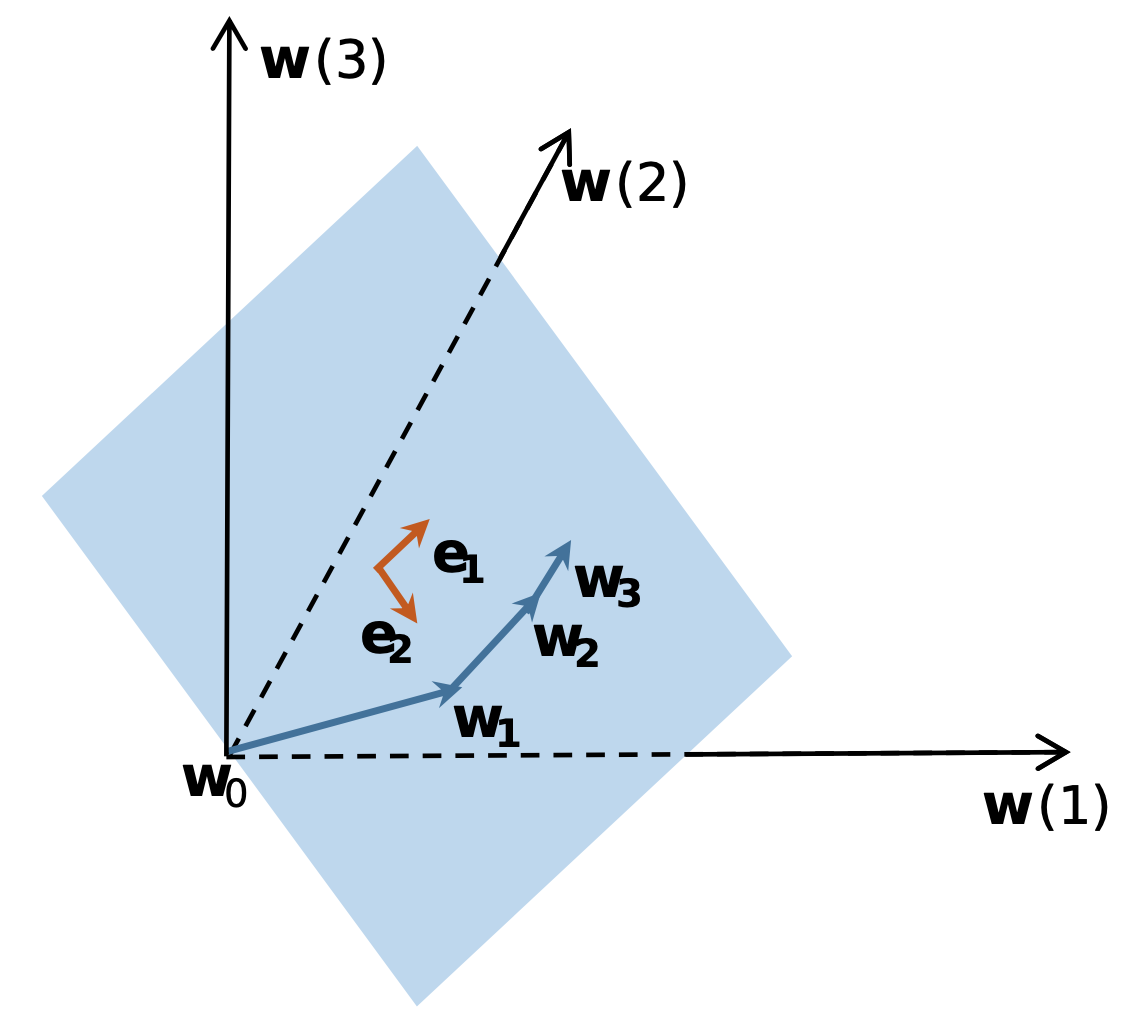
\includegraphics[width=0.5\linewidth]{images/trajectory.png}
\caption{Low-dimensional optimization trajectory}
\label{fig:trajectory}
\end{figure}  

Figure \ref{fig:trajectory} visualizes a three-dimensional space containing three variables $w(1)$, $w(2)$, $w(3)$. These refer to the optimizable parameters of a very basic neural network. By training this network for three iterations, one achieves an optimization trajectory $(w_k)_{k=0}^3$, that could be embedded in a two-dimensional hyperplane, spanned by the orthogonal vectors $e_1$ and $e_2$. \\

Theoretically, this basic idea could translate to higher-dimensional models and more complex affine sets as well. Note that none of the optimizable variables could be left out to reduce the dimension, but rather one has to construct new independent variables to obtain the lower-dimensional affine set that approximately contains the optimization trajectory.  \\

If the low-dimensional trajectory hypothesis holds true, it would provide a new understanding of neural networks, both from a theoretical and practical perspective. According to \cite{Paper}, this includes generalization capability, implicit regularization, efficient learning algorithms and much more. Furthermore there would be benefits like the possibility to use second-order methods for optimization in case the optimization trajectory's dimension is small enough. \\

We start by investigating the low-dimensional trajectory hypothesis from a theoretical perspective. This is based on the following background knowledge on the singular value decomposition (SVD) and low-rank approximations.

\subsection{Singular Value Decomposition}

The following result is denoted and proven as theorem 2.5.2 in \cite{SVD}.

\begin{theorem}[Singular Value Decomposition] \label{thm:svd}
For every matrix $A \in \R^{m \times n}$ there exist orthogonal matrices $U \in \R^{m \times m}$ and $V \in \R^{n \times n}$ and a diagonal matrix 
\[ \Sigma \coloneq \text{diag}(\sigma_1, \dots, \sigma_p) \in \R^{m \times n} \]
with $p \coloneq \text{min} \{ m,n \}$ and singular values $\sigma_1 \geq \sigma_2 \geq \cdots \geq \sigma_p \geq 0$, such that
\[ A = U \Sigma V\tr . \]
\end{theorem}

Note that orthogonal matrices refer to real square matrices, whose columns are orthogonal unit vectors. Some authors call these kind of matrices orthonormal and do not demand the unity of columns for a matrix to be orthogonal. However we will stick to the notation in \cite{SVD}. In other words, $Q \in \R^{n \times n}$ is called an orthogonal matrix, if and only if 
\[ Q \tr Q = I_n = Q Q \tr. \]

The SVD decomposes any real valued matrix in a product of three special matrices. This representation yields the singular values which, like eigenvalues, characterize important properties of a matrix. For the further course we need the following definition.

\begin{definition}
The columns of the matrix $U = [u_1, \dots, u_m]$ are referred to as left singular vectors and the columns of the matrix $V = [v_1, \dots, v_n]$ are referred to as right singular vectors.
\end{definition}

Theorem \ref{thm:svd} shows that the sequence of singular values is unique, since they are sorted in descending order. However, the matrices $U$ and $V$ do not have to be unique. For example, the corresponding singular vectors can be interchanged if there are two identical singular values, such that a matrix can have several singular value decompositions. \\

As a simple implication of theorem \ref{thm:svd}, we can denote the following corollary to establish a useful connection between the left and right singular vectors. 

\begin{corollary} \label{cor:svd}
Let $A \in \R^{m \times n}$ be a matrix with singular value decomposition $A=U \Sigma V\tr $, such that $p \coloneq \text{min}\{m,n\}$ and $\sigma_1 \geq \dots \geq \sigma_r > \sigma_{r+1} = \dots = \sigma_p = 0$ for $r \leq p$.
\begin{itemize}
\item[1.] Denoting the columns of $U$ and $V$ with $u_i$ and $v_i$, we have
\[ A v_i = \sigma_i u_i, \quad A\tr  u_i = \sigma_i v_i, \quad i=1,\dots,p.\]
\item[2.] The squares of the singular values $\sigma_1^2, \dots, \sigma_r^2$ are the eigenvalues of $A\tr A$ to the corresponding eigenvectors $v_1, \dots, v_r$.
\end{itemize}
\end{corollary}

\begin{proof}
\ 
\begin{itemize}
\item[1.] Using $A=U \Sigma V\tr $ and the orthogonality of $V$ we derive
\[ Av_i = U \Sigma V\tr  v_i = U \Sigma e_i = U \sigma_i e_i = \sigma_i u_i \]
for $i=1, \dots, p$. Analogously we conclude the second statement
\[ A\tr  u_i = V \Sigma U\tr  u_i = V \Sigma e_i = V \sigma_i e_i = \sigma_i v_i. \]
\item[2.] Since $A\tr A$ is symmetric, its spectral decomposition is given by
\[ A\tr A = V \Sigma\tr  U\tr  U \Sigma V\tr  = V \Sigma\tr  \Sigma V\tr  = V \Sigma\tr  \Sigma V^{-1}. \]
Using $\Sigma\tr  \Sigma = \text{diag}(\sigma_1^2, \dots, \sigma_r^2, 0, \dots, 0) \in \R^{n \times n}$ we conclude the corollary. \qedhere
\end{itemize}
\end{proof}

The SVD is an excellent tool to find low-rank approximations of a matrix $A \in \R^{m \times n}$, that is to find a matrix $B \in \R^{m \times n}$ with $\text{rank}(B) < \text{rank}(A)$ such that $\|A -B\|$ is small for some given matrix norm. We can generate such a low-rank approximation by simply reducing the number of singular values in the singular value decomposition.

\begin{definition} \label{def:rank}
Let $A \in \R^{m \times n}$ be a matrix with singular value decomposition $A=U \Sigma V\tr $. For $d < r = \text{rank}(A)$ we define an approximation of $A$ as
\[ A_d \coloneq \sum_{i=1}^{d} u_i \sigma_i v_i\tr  = U_d \Sigma_d V_d \tr , \]
where $U_d \coloneq [u_1, \dots, u_d]$, $V_d \coloneq [v_1, \dots, v_d]$ and $\Sigma_d \coloneq \text{diag}(\sigma_1, \dots, \sigma_d)$.
\end{definition}

In terms of the spectral norm $\| \cdot \|_2$, the matrix $A_d$ is the best possible rank-$d$ approximation. The underlying result is the following, which is denoted and proven as theorem 2.5.3 in \cite{SVD}.

\begin{theorem}[Eckart-Young-Mirsky] \label{thm:eym}
Let $A \in \R^{m \times n}$ be a matrix with singular value decomposition $A= U \Sigma V\tr $. For every $d < r = \text{rank}(A)$ it holds, that
\[ \min_{\text{rank}(B)=d} \big \| A-B \big \|_2 = \big \| A - A_d \big \|_2 = \sigma_{d+1}. \]
\end{theorem}

This concludes the necessary background knowledge on singular value decompositions and low-rank approximations, which will play an important role for the subspace extraction.

\subsection{Low-Dimensional Trajectory Hypothesis}

To provide a mathematical formulation of the low-dimensional trajectory hypothesis, we need the concept of orthogonal projections. The following result is based on section 2.6.1 in \cite{SVD}.

\begin{lemma} \label{lem:orthProjection}
Let $S \subseteq \R^n$ be a subspace. There exists a unique matrix $P \in \R^{n \times n}$, such that
\[ \text{Im}(P) = S \ \wedge \ P^2 = P = P\tr . \]
 The linear map $\tilde{P} : \R^n \to \R^n : x \mapsto Px$ is called the orthogonal projection onto $S$.
\end{lemma}

\begin{proof}
To prove the existence of an orthogonal projection, we let $d \coloneq \text{dim}(S)$ denote the dimension of $S$ and $Q \coloneq [q_1, \dots, q_d] \in \R^{n \times d}$ denote an orthonormal basis of $S$. We define
\[ P \coloneq QQ\tr  \in \R^{n \times n} \]
and observe by the orthonormality of $Q$, that $Q\tr Q = I_d$. Thus $P$ is idempotent, this is
\[ P^2 = QQ\tr QQ\tr = Q I_d Q\tr = QQ\tr = P. \]
Furthermore $P$ is symmetric, since 
\[ P\tr = (QQ\tr)\tr = QQ\tr = P. \]
By the orthonormality of $Q$, for arbitrary $s \in S$ there exists $\alpha = (\alpha_1, \dots, \alpha_d)\tr \in \R^d$ with
\[ s = \alpha_1q_1 + \dots + \alpha_dq_d = Q\alpha. \]
Based on this we derive $S \subseteq \text{Im}(P)$ since
\[ Ps = QQ\tr s = QQ\tr Q\alpha = QI_d\alpha = Q\alpha =s. \]
Additionally $\text{Im}(P) \subseteq S$ due to the fact, that for $x \in \R^n$, we have $\tilde{\alpha} \coloneq Q\tr x \in \R^d$, so
\[ Px = QQ\tr x = Q\tilde{\alpha} \in S. \]
Thus $\text{Im}(P) = S$. This proves the existence of an orthogonal projection $P$ onto $S$. To prove uniqueness of $P$, we should first note that based on $P^2 = P = P\tr $ we have
\[ \forall x,y \in \R^n : (Px)\tr (y-Py) = x\tr P\tr y - x\tr P\tr Py = x\tr Py - x\tr Py = 0. \]
Using $Px \in S$ for every $x \in \R^n$, we can conclude that 
\[ \forall y \in \R^n : y - Py \in S^\perp \coloneq \big \{ z \in \R^n \mid \forall s \in S : z\tr s = 0 \big \}. \]
Next we let $P_1$ and $P_2$ denote orthogonal projections onto $S$, then for any $z \in \R^n$ we derive
\[ \begin{split}
\big \| (P_1-P_2)z \big \|_2^2 
&= \big \| P_1z -P_2z \big \|_2^2 \\\
&= z\tr P_1\tr P_1z - z\tr P_2\tr P_1z -  z\tr P_1\tr P_2z + z\tr P_2\tr P_2z \\\
&= z\tr P_1z - z\tr P_2\tr P_1z -  z\tr P_1\tr P_2z + z\tr P_2z,
\end{split} \]
where we have used the property $P_i^2 = P_i = P_i\tr $ for $i=1,2$. Since each term on the right-hand side is a real number, we can transpose each term to derive
\[ \begin{split}
\big \| (P_1-P_2)z \big \|_2^2 
&=  z\tr P_1z - z\tr P_2\tr P_1z -  z\tr P_1\tr P_2z + z\tr P_2z \\\
&= (P_1z)\tr z - (P_1z)\tr P_2z - (P_2z)\tr P_1z + (P_2z)\tr z \\\
&= (P_1z)\tr (z-P_2z) + (P_2z)\tr (z-P_1z).
\end{split} \] 
Using $\text{Im}(P_1) = S = \text{Im}(P_2)$, we observe that 
\[ P_1z \in S \ \wedge \ z-P_2z \in S^\perp \ \wedge \ P_2z \in S \ \wedge \ z - P_1z \in S^\perp. \]
Thus the right-hand side of the equality is zero and by the positive definiteness of the norm we conclude $P_1 - P_2 = 0$. This implies $P_1 = P_2$ showing the uniqueness of $P$.
\end{proof}

Based on this we can formulate the low-dimensional trajectory hypothesis mathematically.

\begin{hypothesis}
Given a training trajectory $(w_k)_{k=0}^{t}$ in $\R^n$, there exists $d \ll n$ and a $d$-dimensional subspace $S \subset \R^n$ with an orthonormal basis $Q \in \R^{n \times d}$, such that there is a low-dimensional trajectory $(\alpha_k)_{k=0}^{t}$ in $\R^d$, satisfying 
\[ w_{k+1} - w_k \approx Q(\alpha_{k+1} - \alpha_k), \quad k=0, \dots, t-1. \]
\end{hypothesis}
The hypothesis can be explained as follows. Recalling the illustration in figure \ref{fig:trajectory}, low-dimensional trajectory hypothesis claims the existence of a $d$-dimensional affine set, that approximately covers the parameter trajectory $(w_k)_{k=0}^{t}$ in $\R^n$. More precisely, it claims the existence of some $d$-dimensional subspace $S \subset \R^n$ and some $x \in \R^n$, defining the affine set
\[ x + S \coloneq \big \{ y \in \R^n \mid x - y \in S \big \}, \]
such that the distance between $x + S$ and any of the parameters $w_k$ is very small, that is
\[ \exists s_k \in x + S : \big \| w_k - s_k \big \|_2 \approx 0, \quad k=0, \dots, t. \]
By lemma \ref{lem:orthProjection}, there exists a unique orthogonal projection $P \in \R^{n \times n}$ onto the subspace, so
\[ w_{k+1} - w_k \approx P(w_{k+1} - w_k), \quad k=0, \dots, t-1. \]
Thus we can define the projected low-dimensional trajectory $(s_k)_{k=0}^{t} \coloneq (Pw_k)_{k=0}^{t}$, satisfying
\[ w_{k+1} - w_k \approx P(w_{k+1} - w_k) = s_{k+1} - s_k, \quad k=0, \dots, t-1. \]
Given an orthonormal basis $Q \in \R^{n \times d}$ of $S$, each element of the low-dimensional trajectory can be expressed in terms of its coefficients with regard to the basis $Q$, that is
\[ \exists \alpha_k \in \R^{d}: s_k = V\alpha_k, \quad k=0, \dots, t. \]
As a consequence, the low-dimensional trajectory hypothesis claims, that
\[ w_{k+1} - w_k \approx s_{k+1} - s_k = Q(\alpha_{k+1} - \alpha_k), \quad k=0, \dots, t-1. \]

%Recall, that in contrast to this mathematical formulation, figure \ref{fig:trajectory} illustrated the low-dimensional trajectory in an affine set. Nonetheless, this can be easily obtained by adding an adequate translation to the low-dimensional trajectory $(s_k)_{k=0}^{t}$ in the subspace.

To motivate the low-dimensional trajectory hypothesis from a theoretical perspective, we investigate a single output neural network
\[ f: \R^{n_0} \times \R^n \to \R : (x,w) \mapsto f(x,w). \]
As seen in section \ref{sec:Training} the neural network architecture $f$ induces a function space
\[ \F |_{f} \coloneq \Big \{ f_w : \R^{n_0} \to \R : x \mapsto f(x,w) \mid w \in \R^n \Big \}. \]
In order to train the neural network we let
\[ \X = \big \{ (x_i,y_i) \mid i=1, \dots, m \big \} \subset \R^{n_0} \times \R \] 
denote a training set of size $m \in \N$. Recall that training of $f$ refers to finding an optimal parameter vector $w$, which is accomplished by minimizing the empirical error function
\[ E : \R^n \to \R_+ : w \mapsto \sum_{i=1}^{m} \ell \big (f(x_i,w), y_i \big ), \]
where $\ell$ is a loss function of the form
\[ \ell: \R \times \R \to \R_+ : (x,y) \mapsto \ell(x,y). \]
Note that in comparison to the formulation given in section \ref{sec:Training}, we removed the constant factor $1/m$ in front of the sum, which has no influence on the minimum. Furthermore we chose $\lambda = 0$, that is we do not penalize the complexity of $w$. \\

Under the assumption, that all activation functions in $f$ are differentiable, thus $f$ is differentiable itself, the choice of a differentiable loss function $\ell$ enables us to minimize $E$ via gradient descent. Recall, that based on definition \ref{def:follow} we can analyze the training dynamics with a continuous function $w : [0, \infty) \to \R^n : t \mapsto w_t$, that follows the gradient descent on $E$. To clarify this, since gradient descent performs parameter updates with regard to the rule
\[ w_{k+1} \leftarrow w_k - \eta \cdot \nabla E(w_k), \]
we can let $\eta \to 0$, to derive the equation
\[ \lim_{\eta \to 0} \frac{w_{k+1} - w_k}{\eta} = - \nabla E(w_k). \]
As a consequence, the training dynamics are governed by the differential equation
\[ \partial_tw_t = -\nabla E (w_t ). \]
A basic application of the chain rule yields
\[ \partial_t w_t = -\nabla E (w_t ) = \sum_{i=1}^{m} \nabla_w f(x_i,w_t) \cdot \partial_x \ell \big ( f(x_i,w_t), y_i \big ), \]
where $\partial_x \ell$ denotes the partial derivative of the loss function with respect to the first argument. Note that we are still in the one-dimensional setting, such that $\partial_x \ell$ can equivalently be interpreted as the gradient $\nabla_x \ell$. To explain the main idea of dimensionality reduction, we have to present this gradient flow in terms of vectors and matrices. Therefore we let
\[ \nabla_w f(\X, w_t)\tr \coloneq \Big [ \nabla_wf(x_1,w_t), \dots, \nabla_wf(x_m, w_t) \Big ] \in \R^{n \times m} \]
denote the gradients of $f$ at $w_t$ on the training data set $\X$ and
\[ \nabla_{f(\X,w_t)} E \coloneq \Big [ \nabla_x \ell \big ( f(x_1,w_t), y_1 \big ), \dots, \nabla_x \ell \big ( f(x_m,w_t), y_m \big ) \Big ]\tr \in \R^m \]
denote the gradients of $\ell$ with respect to the first argument. This yields the gradient flow
\[ \partial_tw_t = - \nabla_w f(\X, w_t)\tr \cdot \nabla_{f(\X,w_t)} E. \]

%In order to analyze this optimization  process we define the cost functionals
%\[ \L_i: \F|_f \to \R : f_w \mapsto \ell \big (f_w(x_i),y_i \big ) \]
%for $i=1, \dots,m$, such that the empirical error $E$ can be written as
%\[ E(w) = \sum_{i=1}^{m} \ell \big (f(x_i,w), y_i \big ) = \sum_{i=1}^{m} \ell \big (f_w(x_i), y_i \big ) = \sum_{i=1}^{m} \L_i(f_w). \]


%To investigate the parameter evolution during gradient descent on $E we will use the concept of gradient flows.

%\begin{definition} \label{def:flow}
%The gradient flow according to $E$ is a time dependent function
%\[ w: [0, \infty) \to \R^n : t \mapsto w_t, \]
%that suffices the ordinary differential equation
%\[ \partial_t w_t = - \nabla E(w_t). \]
%\end{definition}

%Since gradient descent performs parameter updates with regard to the update rule
%\[ w_{k+1} \leftarrow w_k - \eta \cdot \nabla E(w_k), \]
%we can let $\eta \to 0$, to derive the equation
%\[ \lim_{\eta \to 0} \frac{w_{k+1} - w_k}{\eta} = - \nabla E(w_k). \]
%Thus, the gradient flow $w$ covers the parameter dynamics during gradient descent on $E$.

%\begin{lemma} \label{lem:flow}
%Let $f: \R^{n_0} \times \R^n \to \R$ be a single-output neural network. During training via gradient descent on $E$, the parameters of $f$ evolve along the differential equation
%\[ \partial_tw_t = - \nabla_wf(\X, w_t)\tr  \cdot \nabla_{f(\X,w)} \L|_{f_{w_t}}, \]
%where 
%\[ \nabla_w f(\X, w_t)\tr  \coloneq \Big [ \nabla_wf(x_1,w_t), \dots, \nabla_wf(x_m, w_t) \Big ] \in \R^{n \times m} \]
%denotes the gradients of $f$ at $w_t$ on the training data set $\X$ and 
%\[ \nabla_{f(\X,w)} \L|_{f_{w_t}} \coloneq \Big [ \nabla \L_1|_{f_{w_t}}(x_1), \dots, \nabla \L_m|_{f_{w_t}}(x_m) \Big ]\tr  \in \R^m \]
%denotes the functional gradients of the costs $\L_i$ at $f_{w_t}$ evaluated on $x_i$ for $i=1,\dots,m$.
%\end{lemma}

%\begin{proof}
%By definition \ref{def:follow} we need to show, that
%\[ \partial_t w_t = - \nabla E(w_t) = - \nabla_wf(\X, w_t)\tr  \cdot \nabla_{f(\X,w)} \L|_{f_{w_t}}. \]
%For arbitrary $w \in \R^n$ we can apply the chain rule to derive the gradient
%\[ \begin{split}
%\nabla E(w) &= \sum_{i=1}^{m} \nabla \ell \big ( f(x_i,w), y_i \big ) \\\
%&= \sum_{i=1}^{m} \nabla f(x_i,w) \cdot \nabla \ell \big ( f(x_i,w), y_i \big ) \\\
%&= \sum_{i=1}^{m} \nabla f(x_i,w) \cdot \nabla \ell \big ( f_w(x_i), y_i \big ) \\\
%&= \sum_{i=1}^{m} \nabla f(x_i,w) \cdot \nabla \L_i |_{f_w}(x_i). 
%\end{split} \]
%Using the definitions from the lemma, this is equivalent to
%\[ \nabla E(w) = \sum_{i=1}^{m} \nabla_w f(x_i,w) \cdot \nabla \L_i |_{f_w}(x_i) = \nabla_wf(\X, w_t)\tr  \cdot \nabla_{f(\X,w)} \L|_{f_{w_t}}. \]
%This completes the proof, since $w$ was chosen arbitrary.
%\end{proof}

%In the infinite width limit, we can apply theorem \ref{thm:linear} to approximate the neural network architecture $f$ as a linear model
%\[ f^\textit{lin}(x, w_t) \approx f(x, w_0) + \nabla_wf(\X,w_0)(w_t-w_0). \]
%This is nothing else than a first order Taylor expansion. However, the key observation is, that in the infinite width limit, the error term converges to zero. Based on this, the differential equation in lemma \ref{lem:flow} can be rewritten as
%\[ \partial_tw_t = -\nabla_wf(\X,w_0)\tr  \cdot \nabla_{f(\X,w)} \L|_{f_{w_t}}, \]
%where the first factor is a constant matrix and the second factor changes over time $t$. \\

Based on this differential equation we can use the previous seen properties of the neural tangent kernel to motivate the existence of low-dimensional optimization trajectories and to explain the approach of dimensionality reduction. For this we notate the parallelized outputs
\[ \tilde{f}: \R^{n} \to \R^m : w \mapsto \Big [ f(x_1,w), \dots, f(x_m,w) \Big ]\tr , \]
such that for given $w \in \R^n$, by definition \ref{def:ntk} the neural tangent kernel translates to
\[ \Theta_{w} = \sum_{i=1}^{n} \partial_{w_i} \tilde{f}(w) \otimes \partial_{w_i} \tilde{f}(w) = \nabla_wf(\X,w) \cdot \nabla_wf(\X,w)\tr. \]
In the setting of theorem \ref{thm:ntk}, we have seen that, in the infinite width limit, the neural tangent kernel converges to a deterministic limiting kernel. Thus, in this limit, we have
\[ \nabla_wf(\X,w_t) \cdot \nabla_wf(\X,w_t)\tr = \Theta_t = \Theta_0 = \nabla_wf(\X,w_0) \cdot \nabla_wf(\X,w_0)\tr, \] 
such that ideally the dynamics of gradient flow are governed by
\[ \partial_tw_t = - \nabla_w f(\X, w_0)\tr \cdot \nabla_{f(\X,w_t)} E, \]
where the first factor is a constant matrix and the second factor changes over time $t$. Thus, if the neural tangent kernel $\Theta_0$ is low-rank, $\nabla_wf(\X,w_0)$ could be approximated by a low-rank matrix, such that the optimization trajectory would be embedded in a low-dimensional affine set. To clarify this, we apply singular value decomposition on $\nabla_wf(\X,w_0)$, such that 
\[ \nabla_wf(\X,w_0) = U_0 \Sigma_0 V_0\tr , \]
where $U_0 \in \R^{m \times m}$ and $V_0 \in \R^{n \times n}$ are orthogonal and $\Sigma_0 = \text{diag}(\sigma_1, \dots, \sigma_m)$ is positive semidefinite. Based on this, the neural tangent kernel can be rewritten as
\[ \Theta_0 = \nabla_wf(\X,w_0) \cdot \nabla_wf(\X,w_0)\tr  = U_0 \Sigma_0 \Sigma_0\tr  U_0\tr, \]
which gives the spectral decomposition of $\Theta_0$. More precisely, we could define
\[ \Sigma^\text{NTK} \coloneq \Sigma_0 \Sigma_0 \tr = \text{diag}(\sigma_1^2, \dots, \sigma_m^2), \]
such that the eigenvalues of $\Theta_0$ are given by $\lambda_i = \sigma_i^2$ for $i=1, \dots, m$.

If $\Theta_0$ is low-rank, we could approximate $\Sigma_0$ by a low-rank matrix $\tilde{\Sigma}_0 = \text{diag}(\sigma_1, \dots, \sigma_d)$, so
\[ \Sigma_0 \approx \tilde{U}_0 \tilde{\Sigma}_0 \tilde{V}_0\tr , \]
where $\tilde{U}_0 \in \R^{m \times d}$ contains the first $d$ columns of an $m \times m$ identity matrix and $\tilde{V}_0 \in \R^{n \times d}$ contains the first $d$ columns of an $n \times n$ identity matrix. Using this approximation, we have
\[ \nabla_wf(\X,w_0) = U_0 \Sigma_0 V_0\tr \approx U_0 \tilde{U}_0 \tilde{\Sigma}_0 \tilde{V}_0\tr  V_0\tr . \]
This is exactly the rank-$d$ approximation from definition \ref{def:rank}. As a consequence, the dynamics of gradient flow are approximately governed by
\begin{equation} \label{eq:flow} \tag{$\ast$}
\partial_t w_t = -\nabla_wf(\X,w_0)\tr  \cdot \nabla_{f(\X,w_t)} E \approx - V_0 \tilde{V}_0 \Big ( \tilde{\Sigma}_0 \tilde{U}_0\tr  U_0\tr  \cdot \nabla_{f(\X,w_t)} E \Big ).
\end{equation}
This gives rise to the low-dimensional trajectory hypothesis. The term $V_0\tilde{V}_0 \in \R^{n \times d}$ refers to the orthonormal basis $Q$ of the $d$-dimensional subspace $S$ and the remaining term in parenthesis describes the projected gradient in terms of its coefficients with regard to the basis $Q$ of $S$. \\

By the Eckart-Young-Mirsky theorem \ref{thm:eym}, the used rank-$d$ approximation in (\ref{eq:flow}) is the best possible and the approximation error in terms of the spectral norm is given by
\[ \Big \| \nabla_wf(\X,w_0) - U_0 \tilde{U}_0 \tilde{\Sigma}_0 \tilde{V}_0\tr  V_0\tr \Big \|_2 = \sigma_{d+1}. \] 
The approximation error in (\ref{eq:flow}) is therefore determined by the singular value decay of the matrix $\nabla_wf(\X,w_0)$ or equivalently, the eigenvalue decay of the neural tangent kernel $\Theta_0$. An extensive analysis of this eigenvalue decay can be found in \cite{Decay1} and \cite{Decay2}. These papers show, that in the infinite width limit, the NTK is indeed low-rank, which theoretically motivates the claim of low-dimensional trajectory hypothesis. \\

From a practical perspective however, the previous discussion is too theoretical since it holds true only in the infinite width limit. Of course, this pre-condition is never given in practical applications. This is why section \ref{sec:Experiments} contains various numerical experiments, that investigate the low-dimensional trajectory with regard to finite width deep neural networks.

\subsection{Dynamic Linear Dimensionality Reduction}

For the practical investigation of low-dimensional trajectory hypothesis we have to provide a method to efficiently extract the low-dimensional optimization trajectory. The key issue in here, consist of finding a suitable dimension $d \in \N$ and an orthonormal basis $Q$ of the $d$-dimensional subspace $S \subset \R^n$ whose translation approximately covers the optimization trajectory. This problem will be addressed via principal component analysis (PCA), which operates based on the following definition.

\begin{definition}
For $d \in \N$ we define the set of rank-$d$ orthogonal projection matrices
\[ \P_d \coloneq \Big \{ P \in \R^{n \times n} \mid \text{rank}(P) = d \ \wedge \ P^2 = P = P\tr  \Big \}. \]
\end{definition}

In the following we fix $d \leq n$ and let $W = [w_1, \dots, w_t] \in \R^{n \times t}$ be a mean-centered data matrix, that is $\sum_{k=1}^{t}w_k=0$. Principal component analysis (PCA) consists of finding the orthogonal projection matrix $P^* \in \P_d$, that minimizes the reconstruction error
\[ \P_d \to \R : P \mapsto \sum_{k=1}^{t} \big \| Pw_k - w_k \big \|_2^2. \]
Equivalently, PCA can be formulated as finding the solution $P^* \in \P_d$, such that
\[ P^* \coloneq \argmin_{P \in \P_d} \big \| PW - W \big \|_F^2, \]
where $\| \cdot \|_F$ denotes the Frobenius norm. Casually speaking, principal component analysis aims to project the original data to a lower-dimensional space while preserving as much information as possible. The following theorem provides a method to solve the PCA problem via singular value decomposition. It can be found as theorem 15.1 in \cite{PCA}.

\begin{theorem} \label{thm:pca}
The PCA solution $P^* \in \P_d$ can be decomposed as
\[ P^* = U_dU_d\tr , \]
where $U_d \in \R^{n \times d}$ is the matrix formed by the first $d$ left singular vectors of $W$.
\end{theorem}

\begin{proof}
Let $P \in \P_d$ be arbitrary. By the linearity of the trace, we observe that
\[ \begin{split}
\big \| PW - W \big \|_F^2 
&= \text{Tr} \big [ (PW-W)\tr (PW-W) \big ] \\\
&= \text{Tr} \big [ W\tr  P^2 W - 2 W\tr PW + W\tr W \big ] \\\
&= \text{Tr} \big [ W\tr W\big ] - \text{Tr} \big [W\tr PW \big ],
\end{split} \]
since $P\tr =P=P^2$ by definition. Using that $\text{Tr} \big [ W\tr W\big ]$ is independent of $P$, we derive
\[ \argmin_{P \in \P_d} = \big \| PW-W \big \|_F^2 = \argmax_{P \in \P_d} \text{Tr} \big [ W\tr PW\big ]. \]
By the proof of lemma \ref{lem:orthProjection}, there exists an orthonormal basis $Q = [q_1, \dots, q_d] \in \R^{n \times d}$ of $\R^d$, such that $P$ can be decomposed as $P=QQ\tr $. Using the invariance of the trace under cyclic permutation and the orthogonality of $Q$, we observe that
\[ \text{Tr} \big [ W\tr PW \big ] = \text{Tr} \big [ W\tr QQ\tr W \big ] = \text{Tr} \big [ Q\tr WW\tr Q \big ] = \sum_{i=1}^{d} q_i\tr WW\tr q_i. \]
To maximize the rightmost expression we perform SVD on $W = U \Sigma V\tr $, such that
\[ WW\tr  = U \Sigma V\tr  V \Sigma\tr  U\tr  = U \Sigma \Sigma\tr  U\tr . \]
Using the notation $Z = U\tr QQ\tr U$ we derive by the invariance under cyclic permutation, that
\[ \text{Tr} \big [ Q\tr WW\tr Q \big ] = \text{Tr} \big [ Q\tr U \Sigma \Sigma\tr  U\tr Q \big ] = \text{Tr} \big [ U\tr QQ\tr U\Sigma \Sigma\tr  \big ] = \text{Tr} \big [ Z \Sigma \Sigma\tr  \big ]. \]
Furthermore, we can conclude that $|Z_{i,j} | \leq 1$ for $i,j=1,\dots,n$, since $Z$ is orthogonal as a product of four orthogonal matrices. This implies the inequality
\[ \text{Tr} \big [ W\tr PW \big ] = \text{Tr} \big [ Z \Sigma \Sigma\tr  ] = \sum_{i=1}^{d} z_{i,i} \sigma_i^2 \leq \sum_{i=1}^{d} \sigma_i^2. \]
The upper bound is attained in the case where $Q = U_d = [u_1, \dots, u_d]$ contains the first $d$ columns of $U$. This follows from corollary \ref{cor:svd}, namely the identity $W\tr u_i = \sigma_iv_i$, providing
\[ \text{Tr} \big [ W\tr PW \big ] = \sum_{i=1}^{d} q_i\tr WW\tr q_i = \sum_{i=1}^{d} u_i\tr WW\tr u_i = \sum_{i=1}^{d} u_i\tr W v_i \sigma_i = \sum_{i=1}^{d} \sigma_i^2. \]
As a consequence, the PCA solution is given by $P^* = U_dU_d\tr$.
\end{proof}

In oder to extract the low-dimensional optimization trajectory it is sufficient to determine the $d$-dimensional subspace $S \subset \R^n$. This can be effectively achieved by the procedure provided in the proof of theorem \ref{thm:pca}. The idea is to sample $t \geq d$ parameter vectors along the optimization trajectory and to determine the orthogonal projection $P$ onto $S$ by PCA. By lemma \ref{lem:orthProjection} this also provides an orthonormal basis of the lower-dimensional subspace. \\

The sampling of $t \geq d$ parameters $\{ w_1, \dots, w_t \}$ along the optimization trajectory can be achieved by training the network via some reasonable iterative optimization method such like SGD. The application of PCA to this data requires centralization. Therefore we let
\[ \overline{w} \coloneq \frac{1}{t} \sum_{i=1}^{t} w_i \]
denote the mean of the samples and define the mean-centered data matrix
\[ W \coloneq \big [ w_1 - \overline{w}, \dots, w_t - \overline{w} \big ] \in \R^{n \times t}. \]
Recall that PCA consists of finding the orthogonal projection matrix $P^* \in \P_d$ defined as
\[ P^* \coloneq \argmin_{P \in \P_d} \big \| PW - W \big \|_F^2. \]
The construction of $P^*$ in the proof of theorem \ref{thm:pca} is straight-forward and also provides an orthonormal basis of the $d$-dimensional subspace $S$. At first we need to determine the right singular vectors $v_1, \dots, v_d$ of $W$. Since $t \ll n$ we apply the second statement of corollary \ref{cor:svd} to efficiently compute $v_1, \dots, v_d$ by the spectral decomposition of $W\tr W \in \R^{t \times t}$. According to the first statement of corollary \ref{cor:svd} these can then be used to derive
\[ u_i = \frac{1}{\sigma_i} Wv_i, \quad i=1, \dots, d. \]
By theorem \ref{thm:pca}, the PCA solution is then given by $P^* = U_dU_d \tr$, where $U_d = [u_1, \dots, u_d]$ is an orthonormal basis of $S$, according to the proof of lemma \ref{lem:orthProjection}. Furthermore, the corresponding orthogonal projection onto the $d$-dimensional subspace $S$ is given by the map
\[ P : \R^n \to \R^n : w \mapsto U_dU_d\tr w. \]
With regard to the illustration in figure \ref{fig:trajectory} one could reverse the centralization to define
\[ \tilde{P} : \R^n \to \R^n : w \mapsto \overline{w} + U_dU_d\tr w, \]
projecting the optimization trajectory onto the lower-dimensional affine set $\overline{w} + S$. Speaking in terms of the low-dimensional trajectory hypothesis, it claims that the optimization trajectory is nearly invariant under transformation with $\tilde{P}$. That is 
\[ \forall t>0: \tilde{P}w_t \approx w_t. \]

In summary, we denote the following algorithm for dimensionality reduction from \cite{Paper}.

\begin{algorithm}
\caption{Dynamic Linear Dimensionality Reduction (DLDR) \textcolor{white}{$\Big |$}} \ \\
\textcolor{white}{$\Big |$}\textbf{Input:} Dimensionality of the subspace $d$, number of samples $t \geq d$ \\
\textcolor{white}{$\Big |$}1: Sample parameter trajectory $(w_k)_{k=1}^{t}$ along the optimization trajectory; \\
\textcolor{white}{$\Big |$}2: Compute the mean $\overline{w} \coloneq \sum_{k=1}^{t} w_k$; \\
\textcolor{white}{$\Big |$}3: Centralize the samples as $W = [w_1-\overline{w}, \dots, w_t - \overline{w}]$; \\
\textcolor{white}{$\Big |$}4: Perform spectral decomposition such that $W\tr W = V \Sigma^2 V^{-1}$;  \\
\textcolor{white}{$\Big |$}5: Obtain the $d$ largest eigenvalues $\big [\sigma_1^2, \dots, \sigma_d^2 \big ]$ with eigenvectors $ \big [v_1, \dots, v_d \big ]$; \\
\textcolor{white}{$\Big |$}6: Determine the singular vectors $u_i = \frac{1}{\sigma_i}Wv_i$ for $i=1, \dots, d$; \\
\textcolor{white}{$\Big |$}7: Return the orthonormal basis $ \big [u_1, \dots, u_d \big ]$ of the subspace;
\end{algorithm}

The complexity of the algorithm is determined by lines 5 and 7. In line 5 we calculate the matrix product $W \tr W$ which is of complexity $\O(t^2n)$ and the complexity of the spectral decomposition is $\O(t^3)$, since $W\tr W \in \R^{t \times t}$. Line 7 contains $d$ products $Wv_i$ which is of complexity $\O(dtn)$. Using $d\leq t$ the total complexity of DLDR is $\O(t^3 + 2t^2n)$. Since $t \ll n$ the time consumption is negligible in comparison to the complexity of training.

\subsection{DLDR-based Training Algorithms}

Assuming that the low-dimensional trajectory hypothesis holds true, not only in the infinite width limit but also for finite wide deep neural networks, we could adopt the training algorithms from section \ref{sec:Training} to perform parameter updates in the lower-dimensional subspace. \\

Recall, that all of the proposed training algorithms operate in a similar manner, which consist of iterative parameter updates. This is achieved by computing a descent direction $d_k \in \R^n$, choosing a learning rate $\eta > 0$ and updating the parameters according to the rule
\[ w_{k+1} \leftarrow w_k - \eta \cdot d_k. \]
Note that the training algorithms differ only in determining the descent directions. The basic idea of an parameter update in the  lower-dimensional subspace $S \subset \R^n$ at step $k \in \N$ is to project the parameters $w_k$ and the descent direction $d_k$ onto $S$ and apply the update rule in the subspace $S$. Given an orthonormal basis $Q$ of $S$ the update rule translates to
\[ w_{k+1} \leftarrow Q \big ( Q \tr w_k - \eta \cdot Q \tr d_k \big ). \]
Using the fact, that $S$ is a subspace, this procedure results in a parameter vector $w_{k+1} \in S$, such that an iterative application can be simplified to the update rule
\[ w_{k+1} \leftarrow w_k - \eta \cdot Q Q \tr d_k. \]
If the dimension of the subspace is small enough, training should happen a lot faster than in the original space. Also, since there are only a few variables to optimize, second-order methods become applicable. Another benefit is, that training in the lower-dimensional space should prevent overfitting and improve robustness to label noises. \\

Based on the stochastic gradient descent algorithm, we can introduce its projected version, performing the parameter updates in a lower-dimensional space as follows.

\begin{algorithm}
\caption{Projected Stochastic Gradient Descent (P-SGD) \textcolor{white}{$\Big |$}} \ \\
\textcolor{white}{$\Big |$}\textbf{Input:} Differentiable $E: \R^n \to \R$, batch size $b \in \N$, number of epochs $N \in \N$, $w_0 \in \R^n$, \\
\textcolor{white}{$\Big |$\textbf{Input:}} orthonormal basis $Q \in \R^{n \times d}$ of the $d$-dimensional subspace \\
\textcolor{white}{$\Big |$}1: \textbf{for} $k=0, \dots, \frac{Nm}{b}$ \textbf{do}: \\
\textcolor{white}{$\Big |$}2: \quad Draw a random subset $\I_k \subset \{1, \dots, m \}$ of size $| \I_k | = b$; \\
\textcolor{white}{$\Big |$}3: \quad Choose a step size $\eta_k > 0$; \\
\textcolor{white}{$\Big |$}4: \quad Set $w_{k+1} \leftarrow  w_k - \eta_k \cdot QQ\tr \nabla E(w_k,\I_k)$; \\
\textcolor{white}{$\Big |$}5: \textbf{end for}
\end{algorithm}

The convergence of projected stochastic gradient descent will be investigated in section \ref{sec:Experiments}. \\

If the dimension of the subspace covering the optimization trajectory is small enough, we could probably use second order information for the training of deep neural networks. To clarify this, we have to recall that in Newton's method, the descent direction was defined as
\[ d_k = - H_E^{-1}(x_k) \nabla E(x_k). \]
As discussed, for large $n$ it is computationally impractical to determine the inverse Hessian. However, based on the low-dimensional trajectory hypothesis, for any $x_k$ there could exist some lower-dimensional version of the Hessian, call it $H_0(x_k) \in \R^{d \times d}$, such that
\[ H_E(x_k) \approx Q H_0(x_k) Q \tr. \]
For small $d$ we could effectively compute the inverse Hessian as
\[ H_E^{-1}(x_k) \approx ( Q H_0(x_k) Q \tr )^\dagger = Q H_0^{-1}(x_k) Q \tr, \]
where $\dagger$ denotes the Moore-Penrose inverse. Doing so would enable us to perform the Newton update in the lower-dimensional subspace via the update rule
\[ w_{k+1} \leftarrow w_k - \eta_k \cdot Q \big (H_0^{-1}(x_k) Q \tr \nabla E(x_k) \big ). \]
The problem with that approach however, is that we are still confronted with the determination of $H_0$. To clarify this, although we only need to optimize $d$ independent variables, this optimization is based on the gradients of parameters in the $n$-dimensional space. As a consequence, we still have to approximate the lower-dimensional inverse Hessians $H_0^{-1}$. One method for this purpose, namely BFGS was already introduced in section \ref{sec:Training}. Finally we can denote the following algorithm, which is a slight modification of algorithm 2 in \cite{Paper}.

\begin{algorithm}
\caption{Projected Broyden-Fletcher-Goldfarb-Shanno (P-BFGS) \textcolor{white}{$\Big |$}} \ \\
\textcolor{white}{$\Big |$}\textbf{Input:} Twice differentiable $E: \R^n \to \R$, batch size $b \in \N$, number of epochs $N \in \N$, \\
\textcolor{white}{$\Big |$\textbf{Input:}} $w_0 \in \R^n$, orthonormal basis $Q \in \R^{n \times d}$ of the $d$-dimensional subspace \\
\textcolor{white}{$\Big |$}1: Initialize $B_0 \leftarrow I_n$; \\
\textcolor{white}{$\Big |$}2: \textbf{for} $k=0, \dots, \frac{Nm}{b}$ \textbf{do}: \\
\textcolor{white}{$\Big |$}3: \quad Draw a random subset $\I_k \subset \{1, \dots, m \}$ of size $| \I_k | = b$; \\
\textcolor{white}{$\Big |$}4: \quad Compute a step size $\eta_k > 0$ using backtracking line search; \\
\textcolor{white}{$\Big |$}5: \quad Set $x_{k+1} \leftarrow x_k - \eta_k \cdot Q B_k Q^T \nabla E(w_k,\I_k)$; \\
\textcolor{white}{$\Big |$}6: \quad Let $s_k = x_{k+1} - x_{k}$ and $y_k = \nabla f(x_{k+1}) - \nabla f(x_{k})$; \\
\textcolor{white}{$\Big |$}7: \quad Let $\rho_k = (y_k\tr s_k)^{-1}$ and $V_k = I_n - \rho_k y_k s_k\tr $; \\
\textcolor{white}{$\Big |$}8: \quad Set $B_{k+1} \leftarrow V_k\tr B_{k}V_k + \rho_k s_k s_k\tr $; \\
\textcolor{white}{$\Big |$}9: \textbf{end for}
\end{algorithm}

Note that the backtracking linesearch in here has to be performed with respect to the gradient in the lower-dimensional subspace. Denoting this lower-dimensional descent direction as
\[ d_k \coloneq Q^T \nabla E \big (w_k,\I_k \big), \] 
the adopted version of backtracking linesearch iteratively searches for some $\eta_k > 0$ satisfying 
\[ E \big (w_k - \eta_k \cdot Q B_k d_k, \I_k \big) \leq E \big (w_k, \I_k \big ) - c \cdot \eta_k \cdot d_k \tr B_k d_k. \]
In this equation we used the minor definition from section \ref{sec:Training}, namely 
\[ E(w_k,\I_k) \coloneq \frac{1}{b} \sum_{i \in \I_k}^{}  \ell \big ( f(x_i,w_k),y_i \big) + \lambda \big \| w_k \big \|_2^2. \]
According to \cite{Paper}, the step size choice via this adopted version of backtracking linesearch ensures $y_k \tr s_k > 0$, which guarantees the positive definiteness of the inverse Hessian approximation $B_{k+1}$. As a consequence, the proposed P-BFGS algorithm is well-defined. Similar to the choice in \cite{Paper}, we always use $c = 0.4$ and $\beta = 0.55$ to perform the backtracking linesearch.

\pagebreak
\section{Numerical Experiments} \label{sec:Experiments}

This section investigates the low-dimensional trajectory hypothesis from a practical perspective. We conduct extensive numerical experiments to study the performance of DLDR-based training algorithms, namely P-SGD and P-BFGS, on various architectures and data sets. In this context, we also analyze the computational complexity of the subspace extraction via DLDR. The experiments include a comparison of different sampling strategies and subspace dimensions. Finally, we propose a technique to effectively find an appropriate space size and use this to introduce a new training algorithm based on P-BFGS. All of the experiments are run on a NVIDIA A100 GPU using PyTorch. \\

As a warm-up, we start with a motivational experiment, indicating that the low-dimensional trajectory hypothesis could indeed hold true. We proceed as in section 3.3 of \cite{Paper} and study the training of ResNet8 \cite{ResNet} on the CIFAR-10 data set. More precisely, we compare the performance of training in a low-dimensional subspace to the performance of training in the full parameter space of dimension 75,290. The data set is normalized by channel-wise mean and variance. Furthermore we apply horizontal flipping with probability of 0.5 as well as cropping and 4-pixel padding. At first we conduct the full parameter training via SGD with learning rate of 0.1, batch size of 128 and momentum of 0.9. During the first 30 epochs of that training, we save the network's parameter vector after each epoch, that is we generate a trajectory $(w_k)_{k=1}^{30}$ in $\R^{75,290}$. In a follow-up experiment, these samples are used to extract a low-dimensional subspace of dimension 15. Note that the choice of this specific dimension is arbitrary and was imitated from section 3.3 of \cite{Paper}. To investigate the low-dimensional trajectory hypothesis from a practical perspective, we then train the same network from scratch, using P-SGD in the 15-dimensional subspace. For reasons of comparability, we start from the same initialization and use the same hyperparameters as for regular SGD.

\begin{figure}[!h]
\centering
\subfigure[] {\label{fig:exp0-acc}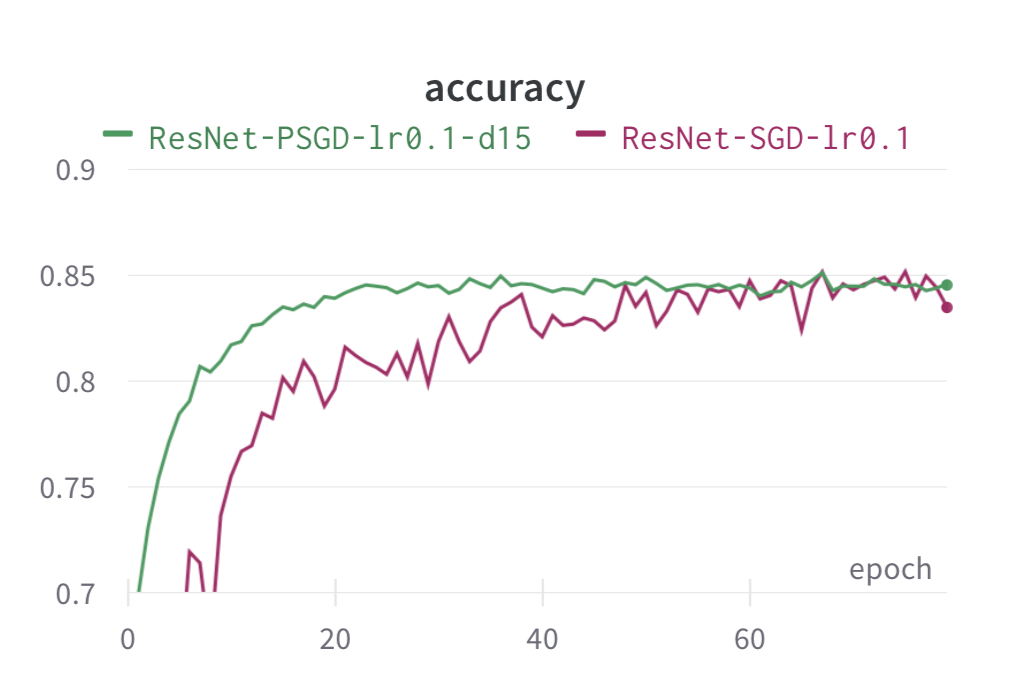
\includegraphics[width=0.4\textwidth]{images/exp0-acc.png}}
\subfigure[] {\label{fig:exp0-pca}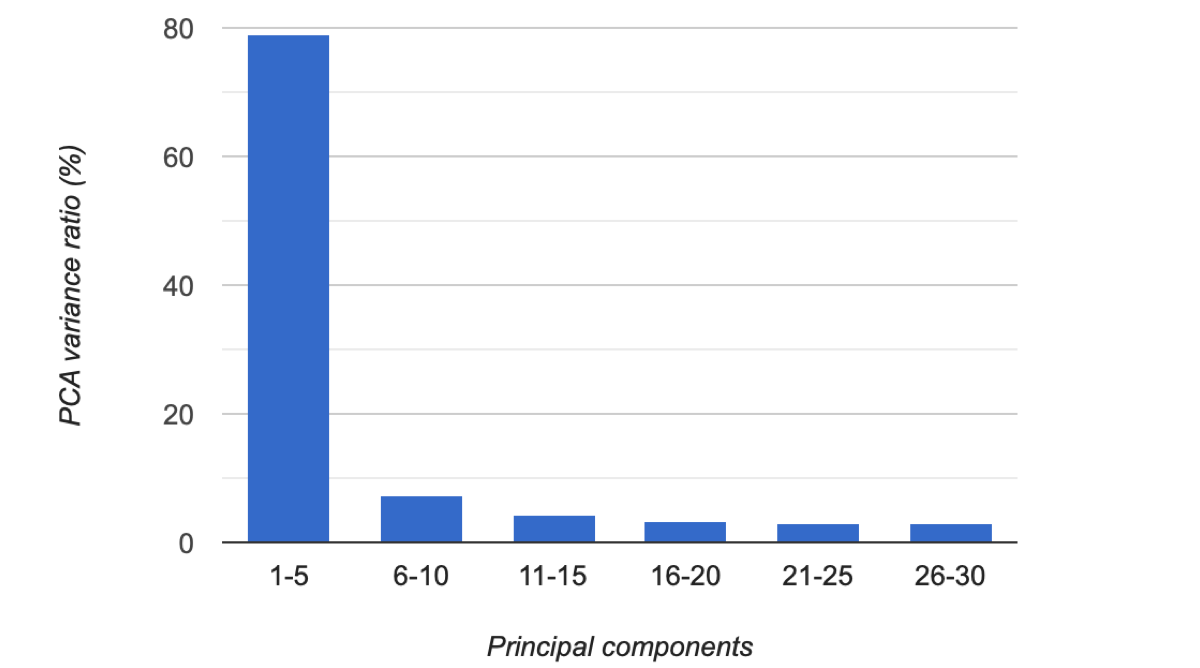
\includegraphics[width=0.4\textwidth]{images/exp0-pca.png}}
\caption{\centering Experiments for ResNet8 on CIFAR-10. (a) Training performance of SGD and P-SGD in 15D subspace. (b) PCA variance ratio of the samples $W = [w_1, \dots, w_{30}]$. }
\label{fig:exp1}
\end{figure}

Figure \ref{fig:exp0-acc} compares the performance of SGD and P-SGD. With 3 runs, SGD obtains averagely 85.??\% test accuracy and P-SGD obtains averagely 85.??\%. Note that within the first 30 epochs of training, the performance of P-SGD is significantly better than the performance of SGD.  This indicates, that P-SGD is able to optimize the parameters by itself, so the good performance isn't a result of the information provided by the sampling stage. Empirically, this simple experiment strongly supports the low-dimensional trajectory hypothesis.

Figure \ref{fig:exp0-pca} illustrates the PCA variance ratio of the sampled parameters $W = [w_1, \dots, w_{30}]$. This concept can be explained as follows. Given a singular value decomposition
\[ W = U \Sigma V\tr, \]
where $\Sigma = \text{diag}(\sigma_1, \dots, \sigma_{30})$, the PCA variance ratio of the $k$-th component is defined as
\[ \frac{\text{variance of component } k}{\text{total variance}} = \frac{\sigma_k}{\sum_{i=1}^{30}\sigma_i}. \]
The fact that the first five components contribute over 90\% to the total variance, indicate that, indeed the optimization trajectory could be embedded in a very low-dimensional affine set. This coincides with the good performance of training in a subspace of dimension 15.

\subsection{Verification on Various Architectures}

Next we verify the previous findings for more complex neural network architectures. Similar to section 5.1 and 5.2 of \cite{Paper}, we train 10 neural network architectures on the CIFAR-100 data set. These include widely known architectures like VGG11, DenseNet121 or GoogLeNet. Just like before we normalize the data set by channel-wise mean and variance and perform the same data augmentations as for CIFAR-10. At first we conduct the full parameter training via SGD with batch size of 128, momentum of 0.9 and weight decay of $10^{-4}$. All of the models are trained for 200 epochs each, using a learning rate of 0.1 for the first 150 epochs.  For the final 50 epochs a reduced learning rate of 0.01 is used. During this training we adopt the same sampling strategy as for the motivational experiment, which is to sample ones after each epoch. However, to allow for a larger subspace dimension we sample the parameters for the first 100 epochs. This setup is imitated from section 5.1 and 5.2 of \cite{Paper}. \\

Table \ref{tab:psgd-1} reports the test accuracy of SGD after training for 50, 100 and 200 epochs. The results are exactly the findings of table 2 in \cite{Paper}. Note that the authors report the actual accuracy after the corresponding number of epochs. For example this can be seen for the SqueezeNet, where the accuracy after 100 epochs is lower than after 50 epochs. In order to ensure a fair comparison to the performance of training in low-dimensional subspaces, instead we consider the maximal test accuracy after 50, 100 and 200 epochs, reported in table \ref{tab:psgd-2}. Comparing the number of parameters in these two tables, we notice slight differences. This is most likely explained by negligence in \cite{Paper} and irrelevant for the further analysis. \\

After training the models in full parameter space, we conduct further experiments on the existence of low-dimensional optimization trajectories. The detailed approach is to train 40 epochs of P-SGD in a 40-dimensional subspace. Again, the specific choice of dimension 40 is arbitrary and was imitated from \cite{Paper}. Note that this dimension is used for all of the 10 models. The hyperparameter setting is as follows. Similar to regular SGD training we adopt the same batch size of 128 and momentum of 0.9. For P-SGD however, no weight decay is used and the initial learning rate is set to 1, which is reduced to 0.1 after the first 30 epochs. For reasons of comparability, SGD and P-SGD start with the same initialization. The maximal test accuracy, when using the first 50 or the first 100 samples for subspace extraction is reported in table \ref{tab:psgd-2}. Note that these are two different subspaces, so two independent optimizations, that should not be confused with the sequential results reported for regular SGD training. 

\begin{table}
\begin{tabu} to \textwidth { l | r | X[c] X[c] X[c] | X[c] X[c] }
\hline \hline \multicolumn{7}{c}{} \\ [-2.5ex]
\textcolor{white}{$\Big |$} & & \multicolumn{3}{c|}{SGD} & \multicolumn{2}{c}{P-SGD} \\
\textcolor{white}{$\Big |$}model & \#params & \multicolumn{3}{c|}{\#training epochs} & \multicolumn{2}{c}{\#sampling epochs} \\
\textcolor{white}{$\Big |$}& & 50 & 100 & 200 & 50 & 100 \\
\multicolumn{7}{c}{} \\ [-2.5ex] \hline \multicolumn{7}{c}{} \\ [-2.5ex]
\textcolor{white}{$\Big |$}SqueezeNet \cite{SqueezeNet} & 0.78M & 59.52 & 58.56 & 70.29 & 69.89 & 70.60 \\
\textcolor{white}{$\Big |$}ShuffleNetv2 \cite{ShuffleNet} & 1.3M & 62.90 & 63.15 & 72.06 & 71.34 & 72.29 \\
\textcolor{white}{$\Big |$}MobileNet \cite{MobileNet} & 3.3M & 57.15 & 58.67 & 67.94 & 66.86 & 68.00 \\
\textcolor{white}{$\Big |$}EfficientNet \cite{EfficientNet} & 4.14M & 62.53 & 63.68 & 72.94 & 71.68 & 72.64 \\
\textcolor{white}{$\Big |$}GoogLeNet \cite{GoogLeNet} & 6.2M & 62.32 & 66.32 & 76.88 & 75.66 & 77.27 \\
\textcolor{white}{$\Big |$}DenseNet121 \cite{DenseNet} & 7.0M & 65.39 & 64.57 & 76.76 & 74.25 & 76.34 \\
\textcolor{white}{$\Big |$}SEResNet18 \cite{SEResNet} & 11.4M & 64.74 & 64.68 & 74.95 & 74.33 & 75.09 \\
\textcolor{white}{$\Big |$}Xception \cite{Xception} & 21.0M & 64.57 & 65.81 & 75.47 & 75.68 & 75.56 \\
\textcolor{white}{$\Big |$}Inceptionv3 \cite{Inception} & 22.3M & 61.68 & 64.00 & 76.25 & 75.15 & 76.83 \\
\textcolor{white}{$\Big |$}VGG11\_bn \cite{VGG} & 28.5M & 58.38 & 59.90 & 68.87 & 68.72 & 70.18 \\
\multicolumn{7}{c}{} \\ [-2.5ex] \hline \hline
\end{tabu}
\centering \parbox{12cm}{\caption{\centering Test accuracy on CIFAR-100 using regular SGD training and P-SGD training in 40-dimensional subspaces. Source: Table 2 in \cite{Paper}.}\label{tab:psgd-1}}
\end{table}

\begin{table}
\begin{tabu} to \textwidth { l | r | X[c] X[c] X[c] | X[c] X[c] }
\hline \hline \multicolumn{7}{c}{} \\ [-2.5ex]
\textcolor{white}{$\Big |$}& & \multicolumn{3}{c|}{SGD} & \multicolumn{2}{c}{P-SGD} \\
\textcolor{white}{$\Big |$}model & \#params & \multicolumn{3}{c|}{\#training epochs} & \multicolumn{2}{c}{\#sampling epochs} \\
\textcolor{white}{$\Big |$}& & 50 & 100 & 200 & 50 & 100 \\
\multicolumn{7}{c}{} \\ [-2.5ex] \hline \multicolumn{7}{c}{} \\ [-2.5ex]
\textcolor{white}{$\Big |$}SqueezeNet \cite{SqueezeNet} & 0.78M & 60.91 & 62.44 & 71.38 & & \\
\textcolor{white}{$\Big |$}ShuffleNetv2 \cite{ShuffleNet} & 1.36M & 64.55 & 64.74 & 72.34 & & \\
\textcolor{white}{$\Big |$}MobileNet \cite{MobileNet} & 3.32M & 57.99 & 59.95 & 68.01 & & \\
\textcolor{white}{$\Big |$}EfficientNet \cite{EfficientNet} & 4.14M & 61.69 & 63.74 & 72.80 & & \\
\textcolor{white}{$\Big |$}GoogLeNet \cite{GoogLeNet} & 6.40M & 64.86 & 66.32 & 76.26 & & \\
\textcolor{white}{$\Big |$}DenseNet121 \cite{DenseNet} & 7.05M & 66.15 & 67.39 & 77.62 & & \\
\textcolor{white}{$\Big |$}SEResNet18 \cite{SEResNet} & 11.31M & 66.30 & 67.22 & 75.20 & & \\
\textcolor{white}{$\Big |$}Xception \cite{Xception} & 21.01M & 66.79 & 67.14 & 75.63 & & \\
\textcolor{white}{$\Big |$}Inceptionv3 \cite{Inception} & 22.32M & 65.75 & 67.58 & 76.53 & & \\
\textcolor{white}{$\Big |$}VGG11\_bn \cite{VGG} & 28.52M & 59.51 & 61.72 & 68.58 & & \\
\multicolumn{7}{c}{} \\ [-2.5ex] \hline \hline
\end{tabu}
\centering \parbox{12cm}{\caption{\centering Maximal test accuracy on CIFAR-100 using regular SGD training and P-SGD training in 40-dimensional subspaces.}\label{tab:psgd-2}}
\end{table}

Clearly the experiments indicate a comparable performance of training in a 40-dimensional subspace to training in the full parameter space. These findings are empirically verified for 10 different architectures of various complexity, which strongly supports the existence of low-dimensional optimization trajectories. Comparing the performance of P-SGD for subspaces extracted based on 50 and 100 sampling epochs yields another finding. Generally, the performance of P-SGD seems to be better if the subspace extraction method has access to a longer piece of the regular optimization trajectory. A fact that is not directly visible in the table is the fast convergence of P-SGD. Note that we have used an initial learning rate of 1 which is usually too large for regular SGD training. In the low-dimensional subspace however, there are just a few optimizable variables, such that a larger learning rate seems to be applicable. Exemplary, the fast convergence is visualized for the smallest model (SqueezeNet), the largest model (VGG11) and two medium sized models (DenseNet121 and GoogLeNet) in figure \ref{fig:exp1}. Clearly, P-SGD quickly surpasses the performance of SGD and needs just 10 to 20 epochs to almost reach its peak. These observations also apply to the remaining models.

\begin{figure}[!h]
\centering
\subfigure[Squeezenet] {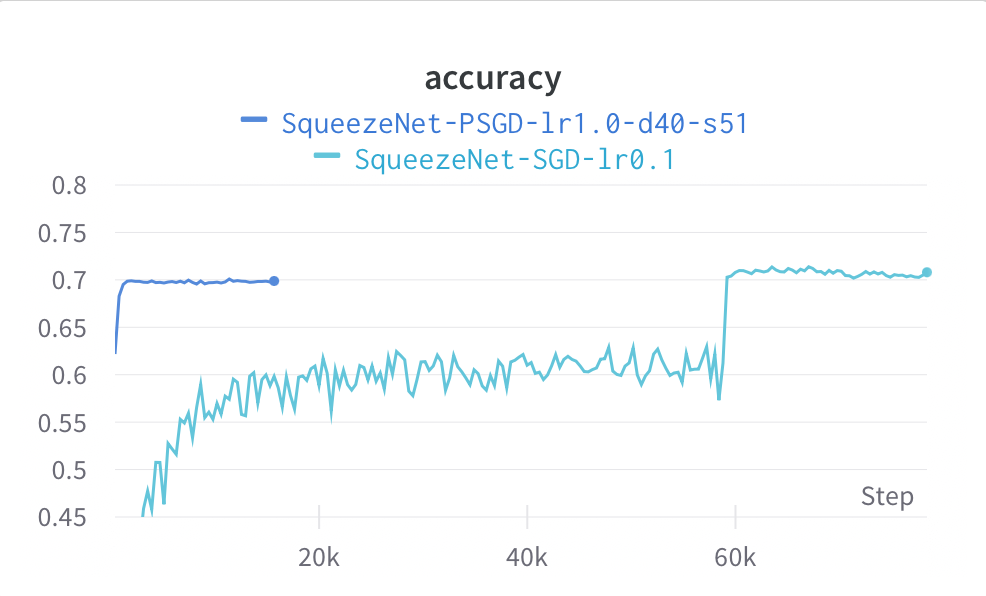
\includegraphics[width=0.44\textwidth]{images/exp1-squeezenet.png}}
\subfigure[GoogLeNet] {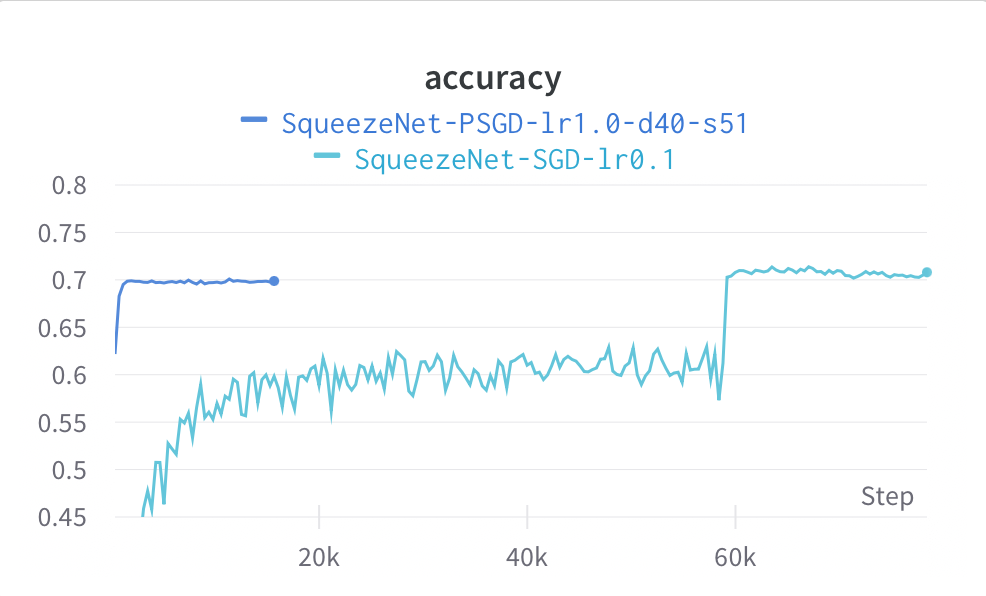
\includegraphics[width=0.44\textwidth]{images/exp1-squeezenet.png}}
\subfigure[DenseNet121] {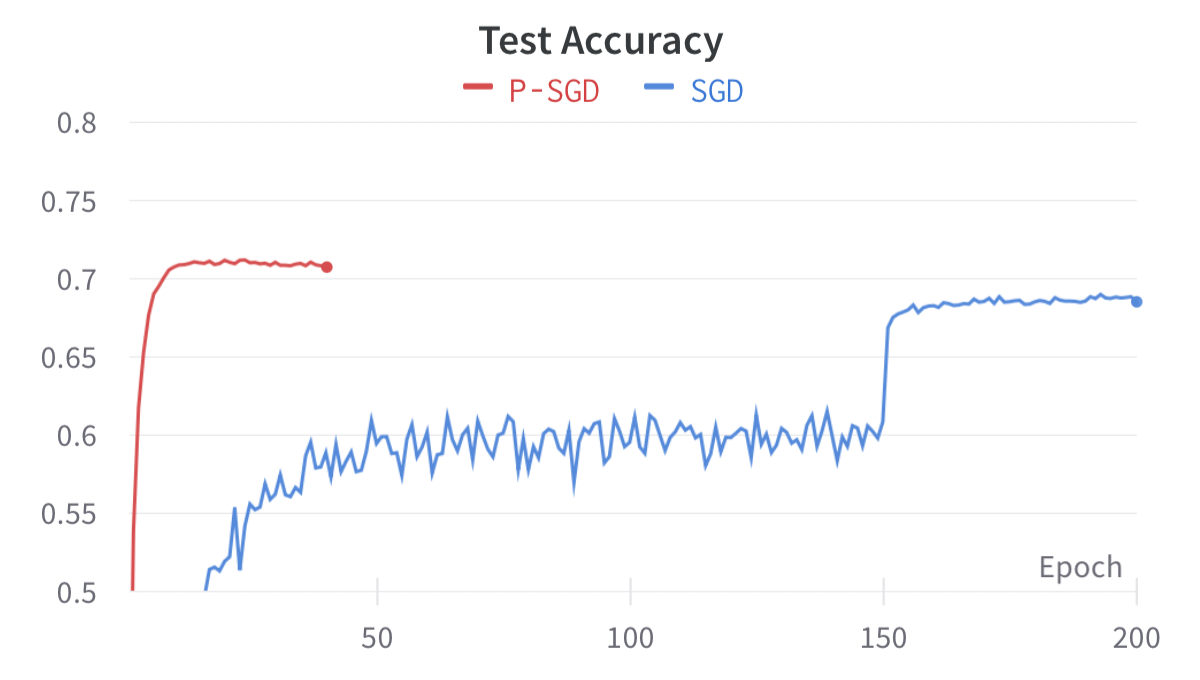
\includegraphics[width=0.44\textwidth]{images/exp1-vgg.png}}
\subfigure[VGG11] {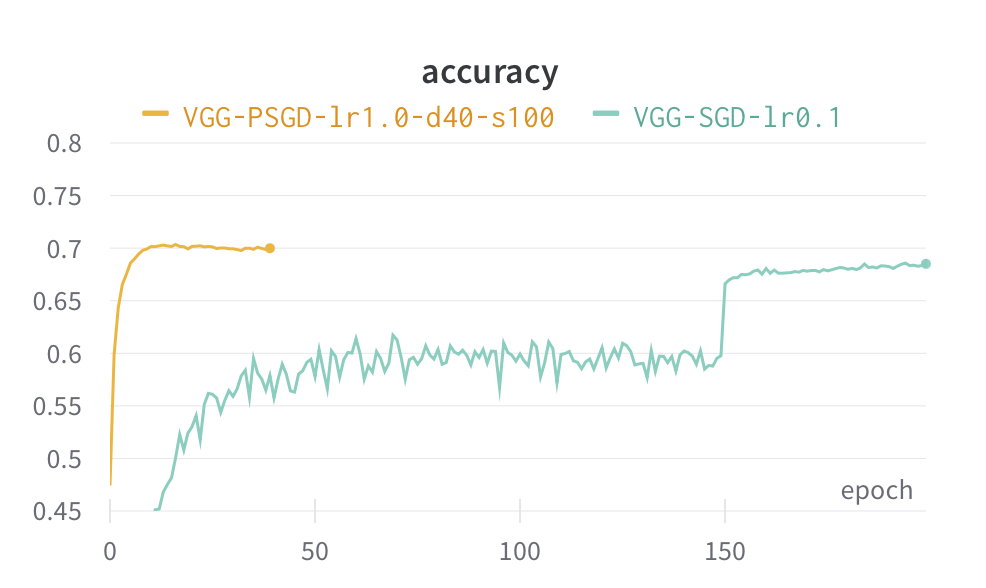
\includegraphics[width=0.44\textwidth]{images/exp1-densenet.png}}
\caption{\centering Training performance on CIFAR-100 using regular SGD training and P-SGD training in 40-dimensional subspaces.}
\label{fig:exp1}
\end{figure}

Next we investigate the computational complexity of DLDR, which includes two major tasks. The first one is to sample parameters along the optimization trajectory using regular SGD. The second one is to perform PCA on these samples. As explained in section \ref{sec:subspaces}, the PCA time consumption should be negligible in comparison to the sampling stage. However, to get a deeper understanding of the computationally complexity, we apply PCA for the optimization trajectories of the 10 previous trained models. The detailed setting is still a fixed subspace dimension of 40, extracted based on various numbers of samples. The computation is conducted on the gpu using torch.pca\_lowrank. Results are reported in table \ref{tab:dldr}.

\begin{table}
\begin{tabu} to \textwidth { l | r | c | X[c] X[c] X[c] X[c] }
\hline \hline \multicolumn{7}{c}{} \\ [-2.5ex]
\multirow{2}{*}{\textcolor{white}{$\Big |$}models}& \multirow{2}{*}{\#params} & training time & \multicolumn{4}{c}{\textcolor{white}{$\Big |$} PCA time for \#samples \textcolor{white}{$\Big |$}} \\
& & \textcolor{white}{$\Big |$} per epoch \textcolor{white}{$\Big |$} &50 & 100 & 150 & 200 \\
\multicolumn{7}{c}{} \\ [-2.5ex] \hline \multicolumn{7}{c}{} \\ [-2.5ex]
\textcolor{white}{$\Big |$}SqueezeNet \cite{SqueezeNet} & 0.78M &  &  &  & \\
\textcolor{white}{$\Big |$}ShuffleNetv2 \cite{ShuffleNet} & 1.36M &  &  &  & \\
\textcolor{white}{$\Big |$}MobileNet \cite{MobileNet} & 3.32M &  &  &  & \\
\textcolor{white}{$\Big |$}EfficientNet \cite{EfficientNet} & 4.14M &  &  &  & \\
\textcolor{white}{$\Big |$}GoogLeNet \cite{GoogLeNet} & 6.40M &  &  &  & \\
\textcolor{white}{$\Big |$}DenseNet121 \cite{DenseNet} & 7.05M &  &  &  & \\
\textcolor{white}{$\Big |$}SEResNet18 \cite{SEResNet} & 11.31M &  &  &  & \\
\textcolor{white}{$\Big |$}Xception \cite{Xception} & 21.01M &  &  &  & \\
\textcolor{white}{$\Big |$}Inceptionv3 \cite{Inception} & 22.32M &  &  &  & \\
\textcolor{white}{$\Big |$}VGG11\_bn \cite{VGG} & 28.52M &  &  &  &  \\
\multicolumn{7}{c}{} \\ [-2.5ex] \hline \hline
\end{tabu}
\centering \parbox{12cm}{\caption{\centering DLDR time consumption in seconds (s) to extract 40-dimensional subspaces for training on CIFAR-100.}\label{tab:dldr}}
\end{table}

Clearly, the computationally complexity is smaller than the complexity of training for one epoch, which is equivalent to generating one sample. This coincides with the theoretical analysis, that DLDR's complexity is negligible in comparison to the sampling stage. \\

Having verified the possible existence of low-dimensional optimization trajectories, we now focus on using these findings to design powerful optimization methods. As of now, training in low-dimensional subspaces was always preceded by a heavy sampling stage based on regular SGD training. As illustrated in figure \ref{fig:exp1}, the actual training in the low-dimensional subspace seems to happen pretty fast. Thus, to design a cost efficient but powerful low-dimensional optimization method, it is key to minimize the computational effort spend on subspace extraction. The key challenge here consists of finding a suitable dimension, generating meaningful samples and performing the PCA. As we have already observed the negligibility of PCA, the upcoming experiments focus on addressing the following two questions.

\begin{center}
Which strategy should be used for sampling? \\
Which subspace dimension should be used for training? \\
\end{center}

\subsection{Subspace exploration}

Two address the two main questions, we compare the performance of training in subspaces of various dimensions using several sampling strategies. We step back to the setting in the motivational experiment, which is training a ResNet8 on CIFAR-10. Hyperparameters are also adopted. For reasons of comparability, in all of these experiments we sample based on the same optimization trajectory of 30 epochs length. However, to allow for larger subspaces and to investigate several sampling strategies, we vary the frequency of samplings per epoch from 1 to 50. This enables us to generate up to 1500 samples during the first 30 epochs of regular training with SGD. Note that with a batch size of 128, one epoch consist of 391 batches, such that a frequency of 50 samples per epoch roughly translates to sampling after 8 batches each. Sampling even more frequently makes no sense, since the distance between samples would become too small. Similar to the motivational experiment, we use these samples to extract the lower-dimensional subspaces. The detailed approach is to test all sampling strategies for training in spaces of various dimensions, ranging from 5 up to 1000. The maximal test accuracy after 40 epochs of training with P-SGD is reported in table \ref{tab:dim}.

\begin{table}[h]
\begin{tabu} to \textwidth { l r | X[c] X[c] X[c] X[c] X[c] X[c] X[c] X[c] | r }
\hline \hline \multicolumn{11}{c}{} \\ [-2.5ex]
& & \multicolumn{8}{c|}{dimension of subspace} & \textcolor{white}{$\Big |$} \\
& & 5 & 10 & 15 & 25 & 50 & 100 & 500 & 1000 & best \textcolor{white}{$\Big |$} \\
\multicolumn{11}{c}{} \\ [-2.5ex] \hline \multicolumn{11}{c}{} \\ [-2.5ex]
\multirow{7}{*}{\rotatebox[origin=c]{90}{\#samples}}
&     30 & 79.99 & 85.08 & 85.09 & 85.08 & - & - & - & - & 85.09 \textcolor{white}{$\Big |$} \\
&     60 & 81.72 & 84.45 & 84.77 & 84.63 & 84.86 & - & - & - & 84.86 \textcolor{white}{$\Big |$} \\ 
&     90 & 79.85 & 83.94 & 84.56 & 84.63 & 84.75 & - & - & - & 84.75 \textcolor{white}{$\Big |$} \\
&   150 & 80.30 & 81.79 & 84.13 & 85.02 & 85.30 & 85.26 & - & - & 85.30 \textcolor{white}{$\Big |$} \\ 
&   300 & 74.27 & 81.04 & 82.49 & 84.03 & 84.80 & 85.24 & - & - & 85.24 \textcolor{white}{$\Big |$} \\
&   900 & 69.97 & 79.15 & 79.31 & 82.81 & 83.83 & 84.42 & 85.03 & - & 85.03 \textcolor{white}{$\Big |$} \\
& 1500 & 76.20 & 80.31 & 81.53 & 82.90 & 84.40 & 84.68 & 85.33 & 85.44 & 85.44 \textcolor{white}{$\Big |$} \\
\multicolumn{11}{c}{} \\ [-2.5ex] \hline \multicolumn{11}{c}{} \\ [-2.5ex]
&  best & 81.72 & 85.08 & 85.09 & 85.08 & 85.30 & 85.26 & 85.33 & 85.44 & 85.44 \textcolor{white}{$\Big |$} \\
\multicolumn{11}{c}{} \\ [-2.5ex] \hline \hline
\end{tabu}
\caption{Maximal test accuracy of ResNet8 trained on CIFAR-10 using P-SGD for 40 epochs.}
\label{tab:dim}
\end{table}
 
The experiment empirically provides three major findings. The first one is based on the last row in table \ref{tab:dim}. Clearly, for ResNet8, there seems to be no big difference in performance when training in a subspace of arbitrary dimension between 10 and 1000. However, this is based on an appropriate sampling strategy, that varies from space to space. Furthermore, the 5-dimensional subspace is too small to cover the optimization trajectory. This coincides with the PCA variance ratios illustrated in figure \ref{fig:exp0-pca}. The second finding is based on the last column of table \ref{tab:dim}. Also, for ResNet8, there seems to be no big difference in performance when using different sampling strategies. However, this is based on an appropriate space size, that varies from strategy to strategy. Note that these two findings strongly relate to each other. The third and final finding is a combination of the previous two findings. Especially for the spaces of dimension 5 to 25 it seems to be the case, that given a fixed dimension of the subspace, the performance is better, when only a small number of samples is used for the subspace extraction. Formulated the other way around, given a fixed number of samples, the performance seems to be better when training in a space of larger dimension. Note that the third finding does not contradict the results in table \ref{tab:psgd-2}, where the performance was better when using more samples. The key difference is that we increase the number of samples during a fixed optimization trajectory of 30 epochs length, where as in table \ref{tab:psgd-2} the optimization trajectory was extended from 50 to 100 epochs, explaining the improved results.

Assuming that the findings in table \ref{tab:dim} translate to other architectures and data sets as well, we can formulate the following two approaches for our purpose of designing a cost efficient but powerful low-dimensional optimization method. Firstly, one should aim to find the smallest subspace dimension providing comparable performance to the full parameter training. Secondly, one should aim to generate only a few but high quality samples in the most cost efficient way. For the latter approach, optimizing cost efficiency translates to training as little epochs of regular SGD as possible. \\

With respect to these two approaches, we conduct a follow-up experiment on ResNet8. Its main focus is to investigate the necessary length of the optimization trajectory used for the subspace extraction. Note that table \ref{tab:psgd-2} already indicates a significant improvement when doubling the length from 50 epochs to 100 epochs. However, in the following experiment we are mainly interested in the early stages of samplings. The detailed procedure is to train ResNet8 via P-SGD for 40 epochs in subspaces of dimension 10, 15 and 25. For the subspace extraction we always use a fixed number of 30 samples. However, these samples are generated with several frequencies, translating to different number of epochs needed in the sampling stage. The results are reported in table \ref{tab:epochs}.

\begin{table} [h]
\centering
\begin{tabu} to 0.8\textwidth { c c c | X[c] X[c] X[c] }
\hline \hline \multicolumn{6}{c}{} \\ [-2.5ex]
\multicolumn{3}{c|}{ \textcolor{white}{$\Big |$} sampling strategy \textcolor{white}{$\Big |$}} & \multicolumn{3}{c}{dimension of subspace} \\
\textcolor{white}{$\Big |$} frequency \textcolor{white}{$\Big |$} & \#epochs & \#samples & 10 & 15 & 25  \\
\multicolumn{6}{c}{} \\ [-2.5ex] \hline \multicolumn{6}{c}{} \\ [-2.5ex]
\textcolor{white}{$\Big |$}   1/epoch \textcolor{white}{$\Big |$} &  30  & 30 & 84.92 & 84.95 & 84.92 \\
\textcolor{white}{$\Big |$}   2/epoch \textcolor{white}{$\Big |$} &  15  & 30 & 83.05 & 83.10 & 83.21 \\ 
\textcolor{white}{$\Big |$}   3/epoch \textcolor{white}{$\Big |$} &  10  & 30 & 81.05 & 81.05 & 81.11 \\
\textcolor{white}{$\Big |$}   5/epoch \textcolor{white}{$\Big |$} &    5  & 30 & 76.38 & 76.69 & 77.06 \\
\textcolor{white}{$\Big |$} 10/epoch \textcolor{white}{$\Big |$} &    3  & 30 & 69.82 & 70.26 & 70.45 \\
\multicolumn{6}{c}{} \\ [-2.5ex] \hline \hline
\end{tabu}
\centering \parbox{10cm}{\caption{\centering Maximal test accuracy of ResNet8 trained on CIFAR-10 using P-SGD for 40 epochs.}}
\label{tab:epochs}
\end{table}

Clearly, the performance decreases when using a smaller piece of the regular optimization trajectory for the subspace extraction. This is bad news for our purpose of cost efficient algorithm design, since the spacial information on the low-dimensional trajectory seems to evolve during the training with regular SGD and is not completely  included in the early epochs of training. Again, this is just an observation for ResNet8 on CIFAR-10. However, since this is a pretty simple task in terms of deep learning scenarios, it is very likely that these inconvenient properties translate to more sophisticated architectures and are even reinforced.


\begin{figure}[h]
\centering
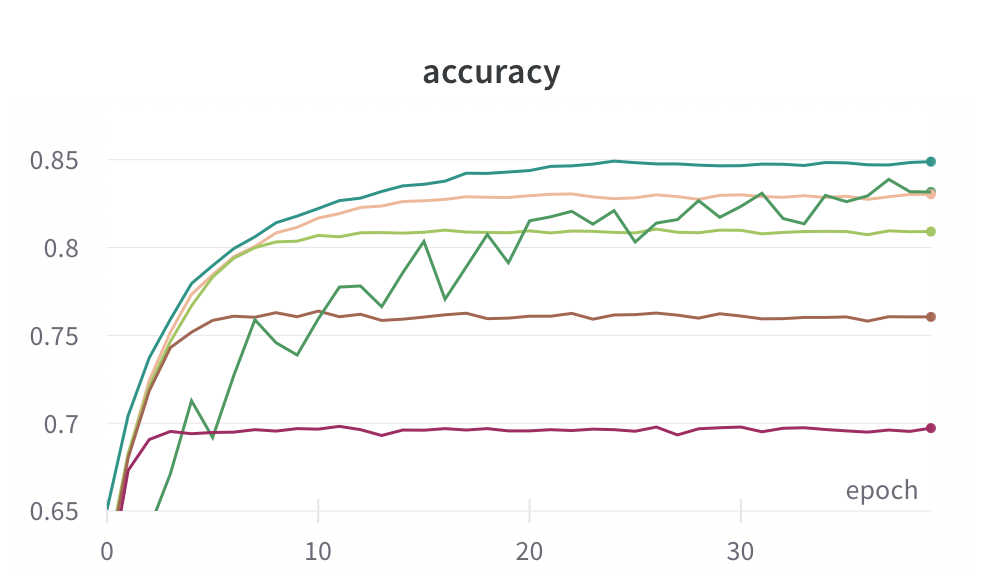
\includegraphics[width=0.6\linewidth]{images/exp1.png}
\caption{Illustration of a neuron as graph.}
\label{fig:a}
\end{figure}

 

 
%\begin{tabu} to \textwidth { r r | X[c] X[c] X[c] | X[c] X[c] X[c] | X[c] X[c] X[c] }
%\hline \hline \multicolumn{11}{c}{} \\ [-2.5ex]
%& \textcolor{white}{$\Big |$} & \multicolumn{3}{c|}{10 epochs} & \multicolumn{3}{c|}{20 epochs} & \multicolumn{3}{c}{40 epochs} \\
%\multicolumn{11}{c}{} \\ [-2.5ex] \hline \multicolumn{11}{c}{} \\ [-2.5ex]
%& \textcolor{white}{$\Big |$} & \multicolumn{3}{c|}{dimension of subspace} & \multicolumn{3}{c|}{dimension of subspace} & \multicolumn{3}{c}{dimension of subspace} \\
%& \textcolor{white}{$\Big |$} & 10 & 15 & 25 & 10 & 15 & 25 & 10 & 15 & 25  \\
%\multicolumn{11}{c}{} \\ [-2.5ex] \hline \multicolumn{11}{c}{} \\ [-2.5ex]
%\multirow{5}{*}{\rotatebox[origin=c]{90}{\#sampling epochs}}
%& \textcolor{white}{$\Big |$} 30 &  &  &  &  &  &  &  &  &  \\
%& \textcolor{white}{$\Big |$} 15 &  &  &  &  &  &  &  &  &  \\ 
%& \textcolor{white}{$\Big |$} 10 &  &  &  &  &  &  &  &  &  \\
%& \textcolor{white}{$\Big |$}   5 &  &  &  &  &  &  &  &  &   \\
%& \textcolor{white}{$\Big |$}   3 &  &  &  &  &  &  &  &  &   \\
%\multicolumn{11}{c}{} \\ [-2.5ex] \hline \hline
%\end{tabu}

\pagebreak
\textbf{Experiment 1:} ResNet8 on CIFAR10 \\
\ \\
- Mention the preliminary work \\
- Compare different space sizes \\
\ \\
$\Rightarrow$ Training is possible in tiny subspaces \\

\subsection{Verification on various architectures}

\textbf{Experiment 2:} 10 models on CIFAR100 \\
\ \\
- Reference results in paper \\
- Compare with own results \\
- Compare DLDR sampling time to SVD computation time \\
\ \\
$\Rightarrow$ Since SVD is only $\sim$ 10\% we focus to improve DLDR sampling \\

\subsection{Iterative space refinement}

\textbf{Experiment 3:} Iterative space refinement \\
\ \\
- Sample after k batches instead each epoch \\
- Measures of distance: increase in accuracy / decrease in loss / ... \\
- TBD \\
\ \\
$\Rightarrow$ Training algorithm that makes use of the low-dimensional trajectory \\

\subsection{Application of second-order information}

\textbf{Experiment 4:} \\
\ \\
- Application of second order methods \\
\ \\
$\Rightarrow$ Second order methods are applicable and efficient \\
\ \\

\pagebreak

%\begin{tabu} to \textwidth { r | X[c] X[c] X[c] X[c] X[c] X[c] X[c] X[c] X[c] X[c] | r }
%\hline \hline \multicolumn{12}{c}{} \\ [-2.5ex]
%& \multicolumn{10}{c|}{\#samples} & \textcolor{white}{$\Big |$} \\
%dim & 30 & 60 & 90 & 120 & 150 & 300 & 600 & 900 & 1200 & 1500 & best \textcolor{white}{$\Big |$} \\
%\multicolumn{12}{c}{} \\ [-2.5ex] \hline \multicolumn{12}{c}{} \\ [-2.5ex]
%    5 & 79.99 & 81.72 & 79.85 & 79.86 & 80.30 & 74.27 & 72.63 & 69.97 & 72.93 & 76.20 & 81.72 \textcolor{white}{$\Big |$} \\
%  10 & 85.08 & 84.45 & 83.94 & 83.14 & 81.79 & 81.04 & 78.28 & 79.15 & 78.65 & 80.31 & 85.08 \textcolor{white}{$\Big |$} \\
%  15 & 85.09 & 84.77 & 84.56 & 83.61 & 84.13 & 82.49 & 79.89 & 79.31 & 81.30 & 81.53 & 85.09 \textcolor{white}{$\Big |$} \\
%  25 & 85.08 & 84.63 & 84.63 & 84.90 & 85.02 & 84.03 & 82.30 & 82.81 & 82.13 & 82.90 & 85.08 \textcolor{white}{$\Big |$} \\
%  50 & - & 84.86 & 84.75 & 84.96 & 85.30 & 84.80 & 84.01 & 83.83 & 84.03 & 84.40 & 85.30 \textcolor{white}{$\Big |$} \\
% 100 & - & - & - & 85.08 & 85.26 & 85.24 & 84.80 & 84.42 & 84.24 & 84.68 & 85.26 \textcolor{white}{$\Big |$} \\
% 500 & - & - & - & - & - & - & 85.11 & 85.03 & 85.27 & 85.33 & 85.33 \textcolor{white}{$\Big |$} \\
%1000 & - & - & - & - & - & - & - & - & 85.22 & 85.44 & 85.44 \textcolor{white}{$\Big |$} \\
%\hline
%best & 85.09 & 84.86 & 84.75 & 85.08 & 85.30 & 85.24 & 85.11 & 85.03 & 85.27 & 85.44 & 85.44 \textcolor{white}{$\Big |$} \\
%\multicolumn{12}{c}{} \\ [-2.5ex] \hline \hline
%\end{tabu}

%\begin{tabu} to \textwidth { l r | X[c] X[c] X[c] X[c] X[c] X[c] X[c] X[c] | r }
%\hline \hline \multicolumn{11}{c}{} \\ [-2.5ex]
%& & \multicolumn{8}{c|}{\#dimension of subspace} & \textcolor{white}{$\Big |$} \\
%& & 5 & 10 & 15 & 25 & 50 & 100 & 500 & 1000 & best \textcolor{white}{$\Big |$} \\
%\multicolumn{11}{c}{} \\ [-2.5ex] \hline \multicolumn{11}{c}{} \\ [-2.5ex]
%\multirow{10}{*}{\rotatebox[origin=c]{90}{\#samples}}
%&     30 & 79.99 & 85.08 & 85.09 & 85.08 & - & - & - & - & 85.09 \textcolor{white}{$\Big |$} \\
%&     60 & 81.72 & 84.45 & 84.77 & 84.63 & 84.86 & - & - & - & 84.86 \textcolor{white}{$\Big |$} \\ 
%&     90 & 79.85 & 83.94 & 84.56 & 84.63 & 84.75 & - & - & - & 84.75 \textcolor{white}{$\Big |$} \\
%&   120 & 79.86 & 83.14 & 83.61 & 84.90 & 84.96 & 85.08 & - & - & 85.08 \textcolor{white}{$\Big |$} \\ 
%&   150 & 80.30 & 81.79 & 84.13 & 85.02 & 85.30 & 85.26 & - & - & 85.30 \textcolor{white}{$\Big |$} \\ 
%&   300 & 74.27 & 81.04 & 82.49 & 84.03 & 84.80 & 85.24 & - & - & 85.24 \textcolor{white}{$\Big |$} \\
%&   600 & 72.63 & 78.28 & 79.89 & 82.30 & 84.01 & 84.80 & 85.11 & - & 85.11 \textcolor{white}{$\Big |$} \\ 
%&   900 & 69.97 & 79.15 & 79.31 & 82.81 & 83.83 & 84.42 & 85.03 & - & 85.03 \textcolor{white}{$\Big |$} \\
%& 1200 & 72.93 & 78.65 & 81.30 & 82.13 & 84.03 & 84.24 & 85.27 & 85.22 & 85.27 \textcolor{white}{$\Big |$} \\ 
%& 1500 & 76.20 & 80.31 & 81.53 & 82.90 & 84.40 & 84.68 & 85.33 & 85.44 & 85.44 \textcolor{white}{$\Big |$} \\
%\hline
%&  best & 81.72 & 85.08 & 85.09 & 85.08 & 85.30 & 85.26 & 85.33 & 85.44 & 85.44 \textcolor{white}{$\Big |$} \\
%\multicolumn{11}{c}{} \\ [-2.5ex] \hline \hline
%\end{tabu}

\pagebreak



Comparison to BFGS:
\renewcommand{\arraystretch}{1.1}
\begin{center}
\begin{tabu} to \textwidth { c | r | X[c] | X[c] X[c] | X[c] X[c] }
\hline \hline \multicolumn{7}{c}{} \\ [-2.5ex]
\multirow{3}{*}{model} & \multirow{3}{*}{\#params} & \multicolumn{1}{c|}{SGD} & \multicolumn{2}{c|}{P-SGD} & \multicolumn{2}{c}{P-BFGS} \\
& & \multicolumn{1}{c|}{\#epochs} & \multicolumn{2}{c|}{\#sampling epochs} & \multicolumn{2}{c}{\#sampling epochs} \\
& & 200 & 50 & 100 & 50 & 100 \\
\multicolumn{7}{c}{} \\ [-2.5ex] \hline \multicolumn{7}{c}{} \\ [-2.5ex]
VGG11\_bn & 28.52M & 68.58 & 69.06 & 70.35 & & \\
EfficientNet-B0 & 4.14M & 72.80 & 71.52 & 73.52 & & \\
MobileNet & 3.32M & 68.01 & 67.27 & 68.67 & & \\
DenseNet121 & 7.05M & 77.62 & 75.34 & 76.22 & & \\
Inceptionv3 & 22.32M & 76.53 & 76.33 & 76.39 & & \\
Xception & 21.01M & 75.63 & 75.67 & 75.37 & & \\
GoogLeNet & 6.40M & 76.26 & 75.14 & 76.67 & & \\
ShuffleNetv2 & 1.36M & 72.34 & 72.05 & 72.91 & & \\
SqueezeNet & 0.78M & 71.38 & 69.82 & 71.32 & & \\
SEResNet18 & 11.31M & 75.20 & 74.80 & 75.13 & & \\
\multicolumn{7}{c}{} \\ [-2.5ex] \hline \hline
\end{tabu}
\end{center}
\renewcommand{\arraystretch}{1}

\begin{algorithm}
\caption{Name: TBD \textcolor{white}{$\Big |$}} \ \\
\textcolor{white}{$\Big |$}\textbf{Input:} Differentiable $E: \R^n \to \R$, batch size $b \in \N$, number of epochs $N \in \N$, $w_0 \in \R^n$, \\
\textcolor{white}{$\Big |$\textbf{Input:}} sampling frequency $\xi \in \N$, learning rate $\eta > 0$ \\
\textcolor{white}{$\Big |0$}1: Initialize $k \leftarrow 0$, $Q \leftarrow [ \ ]$, $W \leftarrow [ \ ]$, $d \leftarrow 0$; \\
\textcolor{white}{$\Big |0$}2: \textbf{while} $k<N$ \textbf{do}: \\
\textcolor{white}{$\Big |0$}3: \quad \textbf{for} $i=0, \dots, 7$ \textbf{do}: \\
\textcolor{white}{$\Big |0$}4: \quad \quad Train one epoch of SGD using learning rate $\eta$ and sample $w_1, \dots, w_\xi \in \R^n$; \\
\textcolor{white}{$\Big |0$}5: \quad \quad Set $W \leftarrow W + [w_1, \dots, w_\xi]$; \\
\textcolor{white}{$\Big |0$}6: \quad \quad Set $k \leftarrow k+1$; \\
\textcolor{white}{$\Big |0$}7: \quad \textbf{end for} \\
\textcolor{white}{$\Big |0$}8: \quad Set $d \leftarrow d+5$; \\
\textcolor{white}{$\Big |0$}9: \quad Compute the singular values $\sigma_1, \dots, \sigma_d$ of $W$; \\
\textcolor{white}{$\Big |$}10: \quad Compute the overall variability $\text{var}(W) = \sum_{i=1}^{k+1} (W\tr W)_{i,i}$; \\
\textcolor{white}{$\Big |$}11: \quad \textbf{if} $\sum_{i=1}^{d} \sigma_i \geq 0.99 \cdot \text{var}(W)$ \textbf{do}: \\
\textcolor{white}{$\Big |$}12: \quad Set $Q \leftarrow$ $d$-dimensional basis of $W$; \\
\textcolor{white}{$\Big |$}12: \quad \quad \textbf{break}; \\
\textcolor{white}{$\Big |$}13: \quad \textbf{end if} \\
\textcolor{white}{$\Big |$}14: \textbf{end while} \\
\textcolor{white}{$\Big |$}16: \textbf{while} $k<N$ \textbf{do}: \\
\textcolor{white}{$\Big |$}17: \quad Train one epoch of P-SGD using learning rate $10\cdot\eta$ and basis $Q$; \\
\textcolor{white}{$\Big |$}24: \quad Set $k \leftarrow k+1$; \\
\textcolor{white}{$\Big |$}25: \textbf{end while} \\
\end{algorithm}

\begin{algorithm}
\caption{Name: TBD \textcolor{white}{$\Big |$}} \ \\
\textcolor{white}{$\Big |$}\textbf{Input:} Differentiable $E: \R^n \to \R$, batch size $b \in \N$, number of epochs $N \in \N$, $w_0 \in \R^n$, \\
\textcolor{white}{$\Big |$\textbf{Input:}} sampling frequency $\xi \in \N$, learning rate $\eta > 0$ \\
\textcolor{white}{$\Big |0$}1: Initialize $k \leftarrow 0$, $Q \leftarrow [ \ ]$, $W \leftarrow [ \ ]$, $d \leftarrow 0$; \\
\textcolor{white}{$\Big |0$}2: \textbf{while} $k<N$ \textbf{do}: \\
\textcolor{white}{$\Big |0$}3: \quad \textbf{for} $i=0, \dots, 7$ \textbf{do}: \\
\textcolor{white}{$\Big |0$}4: \quad \quad Train one epoch of SGD using learning rate $\eta$ and sample $w_1, \dots, w_\xi \in \R^n$; \\
\textcolor{white}{$\Big |0$}5: \quad \quad Set $W \leftarrow W + [w_1, \dots, w_\xi]$; \\
\textcolor{white}{$\Big |0$}6: \quad \quad Set $k \leftarrow k+1$; \\
\textcolor{white}{$\Big |0$}7: \quad \textbf{end for} \\
\textcolor{white}{$\Big |0$}8: \quad Set $d \leftarrow d+5$; \\
\textcolor{white}{$\Big |0$}9: \quad Compute the singular values $\sigma_1, \dots, \sigma_d$ of $W$; \\
\textcolor{white}{$\Big |$}10: \quad Compute the overall variability $\text{var}(W) = \sum_{i=1}^{k+1} (W\tr W)_{i,i}$; \\
\textcolor{white}{$\Big |$}11: \quad \textbf{if} $\sum_{i=1}^{d} \sigma_i \geq 0.99 \cdot \text{var}(W)$ \textbf{do}: \\
\textcolor{white}{$\Big |$}12: \quad Set $Q \leftarrow$ $d$-dimensional basis of $W$; \\
\textcolor{white}{$\Big |$}12: \quad \quad \textbf{break}; \\
\textcolor{white}{$\Big |$}13: \quad \textbf{end if} \\
\textcolor{white}{$\Big |$}14: \textbf{end while} \\
\textcolor{white}{$\Big |$}15: Initialize $\text{best\_acc} \leftarrow 0$, $j \leftarrow 0$; \\
\textcolor{white}{$\Big |$}16: \textbf{while} $k<N$ \textbf{and} $j<3$ \textbf{do}: \\
\textcolor{white}{$\Big |$}17: \quad Train one epoch of P-SGD using learning rate $10\cdot\eta$ and basis $Q$; \\
\textcolor{white}{$\Big |$}18: \quad Validate the model and compute the accuracy; \\
\textcolor{white}{$\Big |$}19: \quad \textbf{if} accuracy $>$ best\_acc \textbf{do}: \\
\textcolor{white}{$\Big |$}20: \quad \quad Set best\_acc $\leftarrow$ accuracy; \\
\textcolor{white}{$\Big |$}21: \quad \textbf{else}: \\
\textcolor{white}{$\Big |$}22: \quad \quad Set $j \leftarrow j +1$; \\
\textcolor{white}{$\Big |$}23: \quad \textbf{end if} \\
\textcolor{white}{$\Big |$}24: \quad Set $k \leftarrow k+1$; \\
\textcolor{white}{$\Big |$}25: \textbf{end while} \\
\end{algorithm}



\begin{algorithm}
\caption{Name: TBD \textcolor{white}{$\Big |$}} \ \\
\textcolor{white}{$\Big |$}\textbf{Input:} Differentiable $E: \R^n \to \R$, batch size $b \in \N$, number of epochs $N \in \N$, $w_0 \in \R^n$, \\
\textcolor{white}{$\Big |$\textbf{Input:}} dimension $d \in \N$ of the subspace, learning rate $\eta > 0$ \\
\textcolor{white}{$\Big |0$}1: Initialize $k \leftarrow 0$, $\text{best\_acc} \leftarrow 0$, $W \leftarrow [w_0]$; \\
\textcolor{white}{$\Big |0$}2: \textbf{for} $j=0, \dots, 1.2d \cdot \frac{1}{3}$ \textbf{do}: \\
\textcolor{white}{$\Big |0$}3: \quad Train one epoch of SGD using learning rate $\eta$ and sample $w_1, w_2, w_3 \in \R^n$; \\
\textcolor{white}{$\Big |0$}4: \quad Set $W \leftarrow W + [w_1, w_2, w_3]$; \\
\textcolor{white}{$\Big |0$}5: \quad Validate the model and compute the accuracy; \\
\textcolor{white}{$\Big |0$}6: \quad \textbf{if} accuracy $>$ best\_acc \textbf{do}: \\
\textcolor{white}{$\Big |0$}7: \quad \quad Set best\_acc $\leftarrow$ accuracy; \\
\textcolor{white}{$\Big |0$}8: \quad \textbf{end if} \\
\textcolor{white}{$\Big |0$}9: \quad Set $k \leftarrow k+1$; \\
\textcolor{white}{$\Big |$}10: \textbf{end for} \\
\textcolor{white}{$\Big |$}11: Extract basis $Q$ of the $d$-dimensional subspace using the samples $W$; \\
\textcolor{white}{$\Big |$}12: Initialize $j \leftarrow 0$; \\
\textcolor{white}{$\Big |$}13: \textbf{while} $j<3$ \textbf{do}: \\
\textcolor{white}{$\Big |$}14: \quad Train one epoch of P-SGD using learning rate $10\cdot\eta$ and basis $Q$; \\
\textcolor{white}{$\Big |$}15: \quad Validate the model and compute the accuracy; \\
\textcolor{white}{$\Big |$}16: \quad \textbf{if} accuracy $>$ best\_acc \textbf{do}: \\
\textcolor{white}{$\Big |$}17: \quad \quad Set best\_acc $\leftarrow$ accuracy; \\
\textcolor{white}{$\Big |$}18: \quad \textbf{else}: \\
\textcolor{white}{$\Big |$}19: \quad \quad Set $j \leftarrow j +1$; \\
\textcolor{white}{$\Big |$}20: \quad \textbf{end if} \\
\textcolor{white}{$\Big |$}21: \quad Set $k \leftarrow k+1$; \\
\textcolor{white}{$\Big |$}22: \textbf{end while} \\
\textcolor{white}{$\Big |$}23: Train $N-k$ epochs of SGD with learning rate $\frac{1}{10}\cdot \eta$; \\
\end{algorithm}

\begin{algorithm}
\caption{Name: TBD \textcolor{white}{$\Big |$}} \ \\
\textcolor{white}{$\Big |$}\textbf{Input:} Differentiable $E: \R^n \to \R$, batch size $b \in \N$, number of epochs $N \in \N$, $w_0 \in \R^n$, \\
\textcolor{white}{$\Big |$\textbf{Input:}} dimension $d \in \N$ of the subspace, number of subspace refinements $\rho \in \N$, \\ 
\textcolor{white}{$\Big |$\textbf{Input:}} sampling frequency $\xi \in \N$, learning rate $\eta > 0$ \\
\textcolor{white}{$\Big |0$}1: Initialize $k \leftarrow 0$, $\text{best\_acc} \leftarrow 0$, $W \leftarrow [ w_0 ]$; \\
\textcolor{white}{$\Big |1$}2: \textbf{for} $i=0, \dots, \rho$ \textbf{do}: \\
\textcolor{white}{$\Big |0$}3: \quad \textbf{for} $j=0, \dots, 1.2d \cdot \frac{1}{\xi(\rho+1)}$ \textbf{do}: \\
\textcolor{white}{$\Big |0$}4: \quad \quad Train one epoch of SGD using learning rate $\eta$ and sample $w_1, \dots, w_\xi \in \R^n$; \\
\textcolor{white}{$\Big |0$}5: \quad \quad Set $W \leftarrow W + [w_1, \dots, w_\xi]$; \\
\textcolor{white}{$\Big |0$}6: \quad \quad Validate the model and compute the accuracy; \\
\textcolor{white}{$\Big |0$}7: \quad \quad \textbf{if} accuracy $>$ best\_acc \textbf{do}: \\
\textcolor{white}{$\Big |0$}8: \quad \quad \quad Set best\_acc $\leftarrow$ accuracy; \\
\textcolor{white}{$\Big |0$}9: \quad \quad \textbf{end if} \\
\textcolor{white}{$\Big |$}10: \quad \quad Set $k \leftarrow k+1$; \\
\textcolor{white}{$\Big |$}11: \quad \textbf{end for} \\
\textcolor{white}{$\Big |$}12: \quad Extract basis $Q$ of the $d \cdot \frac{i+1}{\rho+1}$-dimensional subspace using the samples $W$; \\
\textcolor{white}{$\Big |$}13: \quad Initialize $j \leftarrow 0$; \\
\textcolor{white}{$\Big |$}14: \quad \textbf{while} $j<3$ \textbf{do}: \\
\textcolor{white}{$\Big |$}15: \quad \quad Train one epoch of P-SGD using learning rate $10\cdot\eta$ and basis $Q$; \\
\textcolor{white}{$\Big |$}16: \quad \quad Validate the model and compute the accuracy; \\
\textcolor{white}{$\Big |$}17: \quad \quad \textbf{if} accuracy $>$ best\_acc \textbf{do}: \\
\textcolor{white}{$\Big |$}18: \quad \quad \quad Set best\_acc $\leftarrow$ accuracy; \\
\textcolor{white}{$\Big |$}19: \quad \quad \textbf{else}: \\
\textcolor{white}{$\Big |$}20: \quad \quad \quad Set $j \leftarrow j +1$; \\
\textcolor{white}{$\Big |$}21: \quad \quad \textbf{end if} \\
\textcolor{white}{$\Big |$}22: \quad \quad Set $k \leftarrow k+1$; \\
\textcolor{white}{$\Big |$}23: \quad \textbf{end while} \\
\textcolor{white}{$\Big |$}24: \textbf{end for} \\
\textcolor{white}{$\Big |$}25: Train $N-k$ epochs of SGD with learning rate $\frac{1}{10}\cdot \eta$; \\
\end{algorithm}


\pagebreak
\section{Conclusion}

According to Appendix 8 of \cite{Functionals}, more precisely equation (A.26), we have the following chain rule for functionals.

\begin{lemma}
Let $f \in \F$ be differentiable at $x \in \R^{n_0}$ and $\mu : \F \to \R$ be differentiable at $f$. The functional chain rule states, that
\[ \partial_x \mu[f(x)] = \partial_f \mu[\partial_xf(x)] \]
\end{lemma}

To Do: Figure 4 \\

To Do: Check why Z is orthogonal in pca \\

To Do: Check chain rule with Leonardo \\

To Do: Experiments \\

To Do: Introduction, Conclusion \\

In conclusion...

\pagebreak
\begin{thebibliography}{999}

\bibitem{Paper} Tao Li, Lei Tan, Qinghua Tao, Yipeng Liu, Xiaolin Huang. \textit{Low Dimensional Trajectory Hypothesis is True: DNNs can be Trained in Tiny Subspaces}. IEEE Transactions on Pattern Analysis and Machine Intelligence, 2022.

\bibitem{GD} Augustin Cauchy. \textit{M\'{e}thode g\'{e}n\'{e}rale pour la r\'{e}solution des systemes d'\'{e}quations simultan\'{e}es}. Comptes rendus de l'Acad\'{e}mie des sciences, volume 25, pages 536-538, 1847.

\bibitem{ConvexOptimization} Yurii Nesterov. \textit{Introductory Lectures on Convex Optimization}. Applied Optimization, volume 87, 2004.

\bibitem{BFGS} Richard H. Byrd, Jorge Nocedal, Robert B. Schnabel. \textit{Representations of Quasi-Newton Matrices and their Use in Limited Memory Methods}. Mathematical Programming, volume 60(1), pages 129-156, 1994 

\bibitem{SGD} L\'{e}on Bottou, Frank E. Curtis, Jorge Nocedal. \textit{Optimization Methods for Large-Scale Machine Learning}. SIAM Review, volume 60(2), pages 223-311, 2018.

\bibitem{Adam} Diederik P. Kingma, Jimmy Lei Ba. \textit{Adam: A Method for Stochastic Optimization}. International Conference on Learning Representations (ICLR), 2015.

\bibitem{Armijo} Larry Armijo. \textit{Minimization of Functions Having Lipschitz Continuous First Partial Derivatives}. Pacific Journal of Mathematics, volume 16, no. 1, pages 1-3, 1966.

\bibitem{NTK} Arthur Jacot, Franck Gabriel, Cl\'{e}ment Holger. \textit{Neural Tangent Kernel: Convergence and Generalization in Neural Networks}. Advances in Neural Information Processing Systems, volume 31, pages 8571-8580, 2018.

\bibitem{Functionals} Robert G. Parr, Weitao Yang. \textit{Density-Functional Theory of Atoms and Molecules}. International Series of Monographs on Chemistry Books, volume 16, 1989.

\bibitem{FunctionalAnalysis} Erwin Kreyszig. \textit{Introductory Functional Analysis with Applications}. Wiley Classics Library edition, 1989.

\bibitem{RKHS} Charles A. Micchelli, Massimiliano Pontil. \textit{On Learning Vector-Valued Functions}. Neural Computation, 17:177-204, 2005.

\bibitem{Features} Ali Rahimi, Ben Recht. \textit{Random Features for Large-Scale Kernel Machines}. Advances in Neural Information Processing Systems, volume 20, pages 1177-1184, 2017.

\bibitem{SVD} Gene H. Golub, Charles F. Van Loan. \textit{Matrix Computations}. Third edition, 1996.

\bibitem{Decay1} Zhou Fan, Zhichao Wang. \textit{Spectra of the Conjugate Kernel and Neural Tangent Kernel for Linear-Width Neural Networks}. Advances in Neural Information Processing Systems, volume 33, pages 7710-7721, 2020.

\bibitem{Decay2} Amnon Geifman, Abhay Yadav, Yoni Kasten, Meirav Galun, David Jacobs, Ronen Basri. \textit{On the Similarity between the Laplace and Neural Tangent Kernels}. Advances in Neural Information Processing Systems, volume 33,  pages 1451–1461, 2020.

\bibitem{PCA} Mehryar Mohri, Afshin Rostamizadeh, Ameet Talwalkar. \textit{Foundations of Machine Learning}. Second edition, 2018.

\bibitem{ResNet} Kaiming He, Xiangyu Zhang, Shaoqing Ren, Jian Sun. \textit{Deep Residual Learning for Image Recognition}. Proceedings of the IEEE Conference on Computer Vision and Pattern Recognition (CVPR), pages 770-778, 2016.

\bibitem{VGG}

\bibitem{EfficientNet}

\bibitem{MobileNet}

\bibitem{DenseNet}

\bibitem{Inception}

\bibitem{Xception}

\bibitem{GoogLeNet}

\bibitem{ShuffleNet}

\bibitem{SqueezeNet}

\bibitem{SEResNet}

\end{thebibliography}

\pagebreak
$\b:$ bias vector \\
$\w:$ weight vector \\
- \\
$a:$ element of $\A$ \\
$b:$ batch size \\
$c_i:$ constants \\
$d:$ dimension of subspace \\
$d_f:$ descent direction \\
$d_{\F}:$ pseudo metric on $\F$ \\
$d_{\X}:$ metric on input space \\
$d_{\Y}:$ metric on output space \\
$e_i:$ basis elements \\
$f:$ real valued function \\
$g:$ real valued function \\
$h:$ real valued function \\
$\tilde{f}:$ neural network architecture \\
$i:$ several indices \\
$j:$ alternative index \\
$k:$ iteration index \\
$l:$ number of layers in neural network \\
$\ell:$ loss function \\
$m:$ real number / number of training samples \\
$m_k:$ vector in Adam \\
$n_0:$ input dimension of neural network \\
$n_l:$ output dimension of neural network \\
$n_x:$ input dimension of layer \\
$n_y:$ output dimension of layer \\
$n:$ number of parameters in neural network \\
$p:$ $min\{ n, m\}$ in SVD \\
$r:$ rank in SVD \\
$s:$ real valued vector in BFGS, element of subspace $S$ \\
$s_k:$ low-dimensional trajectory \\
$t:$ time \\
$v_k:$ vector in Adam \\
$w:$ parameter vector in neural network \\
$x:$ real valued vector (input) \\
$x':$ real valued vector (input) \\
$y:$ real valued vector (output) \\
$z:$ real valued vector(input) \\
- \\
$\alpha:$ basis factors \\
$\beta_1:$ momentum factor \\
$\beta_2:$ momentum factor \\
$\epsilon:$ small positive scalar \\
$\eta:$ step size \\
$\lambda:$ real valued scalar \\
$\nu:$ neuron \\
$\mu:$ functional \\
$\phi:$ direction in functional derivative \\
$\psi:$ real valued helper function \\
$\rho:$ real value in BFGS\\
$\sigma:$ activation function \\
$\sigma_i:$ singular values \\
- \\
$A:$ real valued matrix \\
$B:$ real valued matrix \\
$C:$ cost functional \\
$B:$ inverse hessian matrix approximation \\
$E:$ empirical error \\
$F:$ realization function \\
$I_n:$ identity matrix \\
$J:$ riesz mapping \\
$K:$ kernel \\
$L:$ lipschitz constant \\
$M:$ real valued matrix \\
$N$: number of epochs \\
$P:$ orthogonal projection \\
$R:$ generalization error \\
$S:$ subspace \\
$T:$ linear operator \\
$U:$ orthogonal matrix \\
$V:$ orthogonal matrix, matrix in BFGS \\
$Q:$ orthogonal matrix \\
$W:$ weight matrix in layer, data matrix in pca \\
$Z:$ orthogonal matrix \\
- \\
$\Phi_K:$ mapping to Hilbert space \\ 
$\Theta:$ neural tangent kernel \\
$\Sigma:$ covariance matrix, diagonal matrix in SVD \\
- \\
$\A:$ subset of $\F$ \\
$\F:$ function space \\
$\F^*$ dual space \\
$\F |_{\tilde{f}}:$ set of neural networks with given architecture \\
$\D:$ probability distribution \\
$\D_x:$ marginal probability distribution \\
$\I:$ set of indices \\
$\H:$ hilbert space \\
$\mathcal{N}:$ normal distribution \\
$\P$: set of projection matrices \\
$\X:$ input space \\
$\Y:$ output space \\
- \\
$\E:$ expected value \\
$\N:$ natural numbers \\
$\mathbb{P}:$ probability \\
$\R:$ real numbers \\

\end{document}
